\graphicspath{{Chapter7/Chapter7Figs/}}

\chapter{A dynamical mTOR-ROS model for irradiation-induced cellular senescence}
\label{chap:A dynamical mTOR-ROS model for cellular senescence}
This chapter describes a systems biology-based investigation on cellular senescence. The presentation focuses on the modelling point of view and only include \emph{in vitro} experimental work necessary for model validation and test. All the \emph{in vitro} experimental data included in this project were collected by Dr Glyn Nelson, supervised by Professor Thomas von Zglinicki, Institute for Ageing and Health, Newcastle University, United Kingdom.

\section{Introduction}
\label{project3-sec:Introduction}
Cellular senescence is a phenomenon characterised by loss of mitosis and the dysregulation of multiple cellular processes. Ageing is associated with a progressive accumulation of DNA damage and reactive oxygen species (ROS) are a major cause of this damage \citep{Finkel2000}. ROS are mostly generated as a by-product of mitochondrial activity in supplying cells with energy \citep{Turrens2003}. ROS are highly reactive and can cause severe damage to macromolecules and organelles, leading to loss of function. As most ROS are generated from the mitochondria, it is not surprising that mitochondrial DNA (mtDNA) is particularly vulnerable and damage leads to impaired mitochondrial function \citep{Passos2007, Shokolenko2009}. Recent studies also showed that telomere dysfunction can compromise mitochondrial function through activation of p53 and consequently repression of PGC-1$\alpha/\beta$ \citep{Sahin2011}. The result is a viscous cycle whereby ROS cause mitochondrial dysfunction which leads to further increases in 
the 
level of ROS. \\
DNA damage and oxidative stress initiate a multitude of signalling pathways which may, in the case that damage is unrepaired, be reinforced through signalling feedback loops. Under such chronic conditions the downstream consequences may ultimately impair cellular function as is the case with the inflammatory response \citep{Passos2010}. Oxidative stress also activates c-Jun N-terminal kinases (JNK), which is responsible for FoxO3 translocation to the nucleus through phosphorylation \citep{Greer2005, Greer2008}. Oxidative stress promotes SIRT1-dependent deacetylation of FoxO3 favouring the transcription of genes controlling cell cycle arrest \citep{Brunet2004, Greer2005}. Moreover, nuclear FoxO3 induces autophagy by expressing autophagic genes LC3, Gabarapl1 and Atg12 \citep{Sengupta2009,VanDerVos2012}. \\
In recent years, interest has increased on the roles of the insulin/TOR signalling pathway in the mechanisms regulating ageing processes. Its importance was first recognised in worms where inhibition of insulin signalling, particularly Akt activity, leading to enhanced transcriptional activity of Daf-16, the homologue of FoxO3a in humans, was shown to extend lifespan \citep{Lee2003, Murphy2003}. In agreement with this, TOR inhibition by caloric restriction or Rapamycin treatment, or AMPK activation by resveratrol or metformin treatment, increases autophagy \citep{Lee2010,Kim2011} and SIRT1 activity \citep{Rodgers2005, Lagouge2006, Canto2009}. In turn, SIRT1-dependent deacetylation activity was shown to suppress p53 \citep{Vaziri2001} and increase transcriptional activity of FoxO3a and activity of PGC-1$\alpha/\beta$ \citep{Rodgers2005, Lagouge2006, Canto2009}. As a consequence, autophagy and mitochondrial biogenesis are promoted, whereas ROS levels are reduced. \\
The network arising from these signalling pathways is clearly complex, especially due to the numerous signalling pathways and regulatory feedbacks. Moreover, it appears that the cellular transition from normal to senescence involves internal dynamical changes which need to be carefully investigated. In this study, we used a systems biology approach to develop the first dynamical model for irradiation-induced cellular senescence as a means to unravel the main processes governing the transition from a healthy to a senescent cell. We used this model to study FoxO3a-dependent mechanisms of regulating mitochondrial fusion and membrane potential. We provide evidence for the importance of two nuclear states of FoxO3a: unphosphorylated and JNK-dependent phosphorylated. The former predominantly triggered Mfn2 and improved mitochondrial membrane potential. The latter mostly acted in response to DNA-damage and oxidative-stress, and promoted cell cycle arrest through p21 signalling which contributes to ROS production. 
This dual role of FoxO3a was critical for determining cellular senescence progression and consolidation. Also, this work showed that new drug-interventions aimed at preventing cellular senescence, should include combinatorial inhibition of the insulin/TOR pathway and JNK/ROS oxidative-stress response.


\section{Results}
\label{project3-sec:Results}

\subsection{A dynamical model for cellular senescence}
\label{project3-subsec:A dynamical model for cellular senescence}
The model presented in Figure \ref{fig:project3_senescence_model} aimed to integrate five key regulators of ageing: insulin-TOR, FoxO3a, DNA damage, reactive oxidative species (ROS), mitochondrial function. The insulin-TOR network was abstracted in order to reproduce Akt, mammalian TOR Complex I (mTORC1) and the mTORC1-p70-S6K-induced negative feedback loop. Akt was responsible for FoxO3a translocation from the nucleus to the cytoplasm and this migration was overridden by JNK activity \citep{Brunet2004, Greer2005, Greer2008}. This resulted in two nuclear FoxO3a states for which no specific assumption was made on their respective downstream activity. Since PGC-1$\alpha/\beta$ is linked to FoxO3a and activated by AMPK, PGC-1$\alpha/\beta$-dependent mitochondrial biogenesis signalling was embedded within FoxO3a-AMPK-Mfn2 signalling, where Mfn2 is indicative of mitochondrial fusion (mitofusin2) \citep{Koshiba2004}, mitochondrial metabolism \citep{Bach2003} and herein mitochondrial biogenesis through PGC-1$\beta$ 
\citep{Soriano2006, Liesa2008}. Therefore, global mitochondrial function was improved by Mfn2, abstracting PGC-1$\alpha/\beta$ activity. Three states of mitochondrial membrane potential (high, low, null) were assumed. Each state contributed to ROS production and total ROS was responsible for mitochondrial membrane potential decrement. ROS also increased DNA damage levels and induced the oxidative stress response through JNK, which promoted FoxO3a translocation from the cytoplasm to the nucleus. Both nuclear FoxO3a states and DNA damage triggered p21 signalling, which led to an increase in ROS production \citep{Passos2010}. p53 was not directly included into the model because its time-course was similar to DNA damage H2A.X foci marker. Finally, p27 and GSK3$\alpha$ activities were monitored as additional readouts.


\subsection{Time-course analysis upon irradiation-induced senescence}
\label{project3-subsec:Time-course analysis upon irradiation-induced senescence}
\emph{In vitro} experimental time course data were collected in MRC5 fibroblast cells for 13 experimental readouts in the network up to 21 days post 20 Gy X-ray irradiation. The \emph{in vitro} data and model simulation upon X-ray irradiation are shown in Figure \ref{fig:project3_senescence_model_timecourses}. Following irradiation, \emph{in vitro} and \emph{in silico} data showed a dramatic increase in DNA damage and oxidative stress responses, and a consequent decrease in mitochondrial membrane potential. Immediately following cellular damage, an Mfn2 response was observed indicative of unphosphorylated nuclear FoxO3a activity combined with AMPK. The increasing levels of AMPK should result in an increase in the levels of PGC-1$\alpha/\beta$, which in turn should promote mitochondrial biogenesis. However, the mitochondrial membrane potential was not restored, despite AMPK activity. The model parameter estimation explained this conflict by attributing differential roles to the two nuclear FoxO3a pools (see 
graphical model in Figure \ref{fig:project3_senescence_model} and predicted nuclear FoxO3a time courses in Figure \ref{fig:project3_fig2_121029b}A). The JNK-phosphorylated nuclear FoxO3a played a more minor role in activating the processes of mitochondrial fusion and biogenesis than the unphosphorylated-state nuclear FoxO3a. In fact, high JNK levels indicated that FoxO3a mainly resided in the nucleus and was phosphorylated on its JNK-dependent sites. However, JNK-phosphorylated FoxO3a interaction with AMPK was reduced in promoting Mfn2, and consequently mitochondrial membrane potential levels were maintained low and unaffected by JNK activity. Interestingly, although ROS levels were maximised and were maintained stable, JNK was only at half of its maximal observed activity and was gradually increasing, highlighting that other factors, such as chronic inflammation as 
regulated by other pathways, may be responsible for further JNK activation. \\
This consideration provided a preliminary understanding about how a senescent state was driven and consolidated. Firstly, DNA damage and ROS production would be responsible for loss of mitochondria function. Secondly, the system would enter a \emph{point of no return}, due to mitochondrial fusion and biogenesis failure, which in this framework was explained by a shift of FoxO3a activity due to JNK high levels. Therefore, JNK-phosphorylated FoxO3a would not respond to AMPK and potentially would not mediate signals with PGC-1$\alpha/\beta$ to correctly activate the processes of mitochondrial fusion and biogenesis. 


\subsection{JNK inhibition promotes cytoplasmic FoxO3a migration and Mfn2}
\label{project3-subsec:JNK inhibition promotes cytoplasmic FoxO3a migration and Mfn2}
To better formalise and test this hypothesis, we perturbed JNK levels in the model at day 0 and then analysed the effects on FoxO3a and FoxO-downstream proteins. These predictions were tested experimentally \emph{in vitro}.\\ 
As a first step, the model predicted that a JNK inhibition of 25-50\% applied at day 0 would correspond to a reduction in JNK-pT183 levels to 48-73\% at 10 days post irradiation. To experimentally test this prediction, cells were treated with 1$\mu$M of the JNK inhibitor SP600125 at day 0. Consistent with this prediction, \emph{in vitro} JNK inhibition measured at 10 days post irradiation showed a reduction in JNK-pT183 levels to 68\%. Thus, this preliminary result indicated that our \emph{in vitro} JNK inhibition at day 0 was between 25 and 50\% of total JNK level (see Figure \ref{fig:project3_fig2_121029b}B and C). Since JNK constrains FoxO3a to reside inside the nucleus, inhibition of JNK would have allowed FoxO3a translocation to the cytoplasm. The model predicted an increment in cytosolic/nuclear FoxO3a ratio between 117\% and 152\% at 10 days post irradiation upon 25-50\% \emph{in silico} JNK inhibition applied at day 0. This result was experimentally confirmed \emph{in vitro} showing an increase in 
cytosolic/nuclear FoxO3a ratio of 140\% (see Figure \ref{fig:project3_fig2_121029b}B and C). Cytosolic FoxO3a levels were increased as Akt-pS473 induced FoxO3a translocation from the nucleus to the cytoplasm and this translocation was opposed by JNK-pT183. A reduction in JNK-levels thereby released the JNK counter-effect of Akt.\\ 
We then investigated downstream of FoxO3a detecting the levels of mTOR-pS2448, which reflects the activation of mTORC1 through Akt, and Mfn2 upon the same JNK inhibition treatment. The model predicted an increase in both mTOR-pS2448 and Mfn2 levels with respect to the control after 3-5 days post irradiation (see Figure \ref{fig:project3_fig2_121029b}D). In addition, the simulation showed that these levels could stabilise if JNK was inhibited by more than 50\%. This prediction was experimentally verified \emph{in vitro} (see Figure \ref{fig:project3_fig2_121029b}E). Under JNK-inhibition treatment, mTOR-pS2448 and Mfn2 levels were significantly higher than the corresponding control levels. Moreover, these curves gradually decreased after 9-11 days, which was predicted by the model when JNK was inhibited at approximately 50\%.\\
These predictions and \emph{in vitro} confirmations indicated that nuclear FoxO3a acted differently depending on whether it was phosphorylated by JNK in response to oxidative stress. Mfn2 levels remained sensitive even after 9-11 days post irradiation upon JNK inhibition treatment. See Figure \ref{fig:project3_collect_jnk_single_perturb} for model predictions of AMPK-pT172, FoxO3a-pS253, JNK-pT183 and mitochondrial membrane potential upon JNK gradual perturbation. Interestingly, the mitochondrial membrane potential increased upon gradual inhibition of JNK, although the original levels at day 0 were not restored.


\subsection{ROS inhibition improves mitochondrial membrane potential}
\label{project3-subsec:ROS inhibition improves mitochondrial membrane potential}
As ROS is a central driver for mitochondria dysfunction we gradually perturbed the variable ROS in the model at day 0 and analysed the effects on mitochondrial membrane potential along the time course.\\
At 15 days post irradiation, model simulation predicted an increase in mitochondrial membrane potential up to 154\% upon ROS scavenging from day 0 (see Figure \ref{fig:project3_fig3_121026b}A). This prediction was experimentally tested \emph{in vitro} by measuring the TMRM/MTG ratio. The mitochondrial membrane potential increased to 149\% with respect to the control. As the model predicted that an increase to 154\% was obtained by reducing the total ROS amount to 50\% at day 0, we could infer that the \emph{in vitro} experimental test scavenged approximatively 50\% of ROS (see Figure \ref{fig:project3_fig3_121026b}B and C).\\
In addition to these prediction-test results, we also theoretically predicted the effects on Akt-pS473, mTOR-pS2448, Mfn2 and AMPK-pT172 upon ROS gradual perturbation (see Figure \ref{fig:project3_collect_ros_single_perturb}). ROS inhibition was responsible for increasing mTOR-pS2448 and consequently decreasing AMPK-pT172, Akt-pS473 and Mfn2. Intriguingly, Mfn2 was again confirmed to lose sensitivity after 9-11 days post irradiation upon ROS scavenging treatment. This result highlighted the fact that, despite ROS inhibition, the levels of Mfn2 were not restored after 9-11 days, suggesting that a ROS inhibition treatment alone was not sufficient.


\subsection{Combinatorial intervention for improving both Mfn2 and mitochondrial membrane potential}
\label{project3-subsec:Combinatorial intervention for improving both Mfn2 and mitochondrial membrane potential}
By applying a JNK gradual inhibition, we predicted and tested an increase in Mfn2 and cytoplasmic FoxO3a levels. Since FoxO3a translocation to the cytoplasm depends on Akt-pS473, the model predicted that an intervention for increasing Mfn2 levels and mitochondrial membrane potential could be a combined JNK-Akt perturbation. In fact, this intervention allowed us full control over the nuclear states of FoxO3a and therefore its downstream signals (see Figure \ref{fig:project3_figure4_121026c}A). Figure \ref{fig:project3_figure4_121026c}B shows the levels of cytoplasmic FoxO3a-pS253, Mfn2 and mitochondrial membrane potential at day 10 upon combined JNK-Akt perturbation applied at day 0. Cytoplasmic FoxO3a-pS253 levels notably increased upon gradual inhibition of JNK and gradual overexpression of Akt. As our focus was to maintain FoxO3a predominantly in the nucleus and we have showed a beneficial effect upon JNK gradual inhibition, we considered the area of JNK-Akt inhibition (see white 
square marked by *) as a region of study. Interestingly, the model predicted that Mfn2 levels significantly increased up to 166\% by reducing the levels of JNK and Akt in combination to 60\% (see arrow inside square). The mitochondrial membrane potential was also predicted to increase to 133\% by applying the same combined inhibition, although it showed dependency on Akt only when the activity of this protein was reduced.\\
The next step was therefore to use this new information together with the previous prediction-test that ROS inhibition improved mitochondrial membrane potential (see Section \ref{project3-subsec:ROS inhibition improves mitochondrial membrane potential}). The idea was to use the benefits of the predicted output for FoxO3a and Mfn2 upon combined JNK-Akt perturbation (see Figure \ref{fig:project3_figure4_121026c}B) as an input for a combined Mfn2-ROS perturbation (see Figure \ref{fig:project3_figure4_121026c}C). From Figure \ref{fig:project3_figure4_121026c}B, we found a way to increase Mfn2 levels by decreasing both JNK and Akt. Therefore, in a combined Mfn2-ROS perturbation we could simply consider the area of Mfn2 hyperactivation (Mfn2 $>$100\%) (see Figure \ref{fig:project3_figure4_121026c}D). This area could be further reduced by two reasons: 
\begin{description}
 \item[R1.] Cytoplasmic FoxO3a-pS253 levels should be at the basal level of 1 (see Figure \ref{fig:project3_figure4_121026c}B and D, magenta/dark blue colour for FoxO3a-pS253);
 \item[R2.] ROS levels should be maintained as low as possible, since ROS inhibition increases mitochondrial membrane potential (as shown in Figure \ref{fig:project3_fig3_121026b}).
\end{description}
From Figure \ref{fig:project3_figure4_121026c}B, reduced levels of FoxO3a-pS253 (bottom-right) determined low levels of Mfn2 (bottom-right), since FoxO3a acted upstream of Mfn2. Therefore, the region could be safely limited along the threshold 1 of FoxO3a (see magenta/dark blue colour for FoxO3a-pS253) which interestingly corresponded to 50\% of ROS levels in agreement with Figure \ref{fig:project3_fig3_121026b} (see regions indicated by ** in Figure \ref{fig:project3_figure4_121026c}D). Accordingly with Figure \ref{fig:project3_fig3_121026b} and R1, a decrease in ROS levels also determined a significative increase in mitochondrial membrane potential upon a combined Mfn2-ROS perturbation. At this point, we investigated the effect on mitochondrial membrane potential at day 10, upon combined ROS-Mfn2 perturbation applied at day 0, on the correspondent region (marked by **). In agreement, we again found a significant increase to 133\% in mitochondrial membrane potential. This predictive result 
indicated that Mfn2 levels and mitochondrial membrane potential could significantly increase by applying a targeted triple inhibition of Akt, JNK and ROS. In contrast to the application of a combined JNK-Akt inhibition, this intervention had the additional benefit that the network was not unbalanced by oxidative stress signals, as ROS levels were maintained low. Moreover, mitochondrial activity promotes ROS production, which can in turn re-activate JNK and decrease membrane potential. Therefore, it was crucial to limit the levels of ROS in order to avoid losing the achieved benefit.\\
Furthermore, the simulated single perturbation of Mfn2 at day 0 along the time course was also investigated (see Figure \ref{fig:project3_collect_mfn2_single_perturb}). Interestingly, by reducing Mfn2, the mitochondrial membrane potential decreased accordingly. Therefore, since the AMP/ATP ratio increased, activated AMPK negatively regulated mTOR-pS2448. In addition, Mfn2 inhibition produced a moderate ROS reduction, caused by a decrease in mitochondrial membrane potential.


\subsection{Time course analysis of combined TOR-ROS perturbation}
\label{project3-subsec:Time course analysis of combined TOR-ROS perturbation}
In the previous section, we outlined an intervention for increasing both Mfn2 levels and mitochondrial membrane potential by applying a triple inhibition of Akt, JNK and ROS. However, it is well known that TOR plays a crucial role in the regulation of autophagy \citep{Lee2010,Kim2011} and Akt-pS473 \citep{Sarbassov2005, Sarbassov2006}. Therefore it was of interest to study the effect of a combined TOR-ROS perturbation, applied at day 0, on Mfn2 and mitochondrial membrane potential. Moreover, it may be that this new double intervention would be able to restore the mitochondrial membrane potential to its original level and avoid potentially toxic high Mfn2 levels.\\
Perturbation of mTORC1 alone produces serious undesired effects in the insulin/TOR signalling pathway. In fact, mTORC1 inhibition reduces mTORC1-p70-S6K-dependent negative feedback to the insulin receptor substrate (IRS) and therefore hyper-activates Akt \citep{Harrington2004, Shah2004}. A cleaner approach was to perturb both the complexes simultaneously by interacting with TOR kinase directly. In the model mTORC2 was abstracted since Akt-pS473 was dependent on both insulin and mTORC1-p70-S6K-negative feedback loop, whereas mTORC2 was sensitive to insulin but not to the negative feedback loop \citep{DallePezze2012a}. Nevertheless, we could still approximate a TOR kinase perturbation by adjusting a global percentage of the initial protein levels for mTORC1 and Akt at the same time. Therefore, the initial levels of the two protein variables, Akt and mTORC1, were increased or decreased together, simulating a TOR kinase inhibition or over-expression, equivalent to affecting both mTORC1 and mTORC2 in the cell 
(using a TOR inhibitor, such as Torin \citep{Liu2011}, treatment).\\
In simulating a double perturbation of the main TOR kinase and ROS, we detected a non-linear qualitative change along the time course of Mfn2 (see Figure \ref{fig:project3_figure5_121026}A, column 1). Two days after irradiation, Mfn2 was predominantly regulated by ROS levels, with little sensitivity to TOR inhibition. At the same time, mitochondrial membrane potential was affected almost equally by both ROS and TOR at lower levels ($<$100\% TOR, ROS), whereas slightly more by ROS at higher levels ($>$100\% TOR, ROS) (see Figure \ref{fig:project3_figure5_121026}A, column 2). As time progressed, Mfn2 levels decreased and became more affected by TOR perturbation rather then ROS. Meanwhile, mitochondrial membrane potential maintained a combined sensitivity to TOR and ROS, although gradually reduced to low levels along the time course. At days 15-21, TOR and ROS perturbation split the Mfn2 response into two 
activation states. One state ($S_1$) was characterised by low levels of ROS ($<$75\% at day 15), the other ($S_2$) by high levels of ROS ($>$100\% at day 15). Whereas ROS divided the space of Mfn2 response, TOR shaped the boundaries of these two states. In $S_2$, the Mfn2 response maintained an equilibrium by increasing ROS and TOR in combination. This state space was thus concave with respect to the two parameters within the explored boundaries. In $S_1$, the Mfn2 response vanished by increasing TOR levels. Therefore, TOR was responsible for the $S_1$ convex space. Interestingly, the $S_1$ state gradually diminished along the time course. Hence, we simulated the Mfn2 response to TOR and ROS perturbations up to 40 days post irradiation, in order to study the evolution of $S_1$. As shown, at day 40 this second state is almost lost due to the extremely low levels of Mfn2. Moreover, in the extreme regions outside of these two states, Mfn2 levels were either very high ($<$10\% of TOR) or very low ($<$10\% of ROS)
 (see left or bottom of the plot). This could be explained because ROS-JNK-dependent oxidative stress response antagonises Akt-dependent translocation of FoxO3a to the cytoplasm, and therefore promotes fusion. \\
The prediction of these two time-dependent states indicated two modalities of intervention to increase Mfn2 levels: one by increasing ROS levels, the other one by reducing them. Since mitochondrial membrane potential was maximised at low levels of ROS, we experimentally tested the model prediction of Mfn2 and mitochondrial membrane potential upon inhibition of TOR, ROS or TOR-ROS. At day 15, the model predicted a similar Mfn2 response upon inhibition of TOR (to 10-25\%) or TOR-ROS (to 10-25\% and to 45-55\%, respectively). This similarity was also found at day 21 (see Figure \ref{fig:project3_figure5_121026}B). These predictions were experimentally tested \emph{in vitro} by inhibiting TOR (to 10-25\%) or TOR-ROS (to 10-25\% and to 45-55\%, respectively) (see Figure \ref{fig:project3_figure5_121026}C). We were not able to test the non linear response of Mfn2 upon combined perturbation of TOR and ROS at day 21, as the predicted signal differences along the sigmoid curves were too small 
($<$20\%). At day 12 the model predicted no significant response of mitochondrial membrane potential upon TOR inhibition (to 10-25\%) or ROS inhibition (to 45-55\%), although both these inhibitions showed a statistically significant increase in membrane potential with respect to the control. In the case of a TOR-ROS combined inhibition (to 10-25\% and 45-55\%, respectively), the model predicted a significant increase in membrane potential with respect to the control or to the single inhibition treatments (see Figure \ref{fig:project3_figure5_121026}D). These predictions were experimentally tested \emph{in vitro} (see Figure \ref{fig:project3_figure5_121026}E), and confirmed the beneficial effect of a double inhibition and the prevailing role of ROS over TOR at low medium doses of treatment.\\
These results show that TOR inhibition is sufficient for increasing Mfn2 and mitochondrial membrane potential levels, but a combined TOR-ROS treatment is more effective for restoring mitochondrial membrane potential.


\section{Discussion}
\label{project3-sec:Discussion}
In the present work, a dynamical model was employed for investigating the dynamical process of irradiation-induced cellular senescence and studying modalities of combined drug interventions in order to reduce progression of ageing in the middle and long term. We hypothesised that FoxO3a existed in the nucleus in at least two states, unphosphorylated FoxO3a and JNK-phosphorylated FoxO3a, and that these two states mediated distinct cellular processes. Nuclear unphosphorylated FoxO3a was mainly responsible for Mfn2 activation and partially for cell cycle arrest, whereas JNK-phosphorylated FoxO3a was mostly responsible for cell cycle arrest. DNA damage and oxidative stress response activated the inflammatory system through JNK and gradually shifted the FoxO3a nuclear system from the unphosphorylated state to the JNK-phosphorylated state. In addition to the initial establishment of positive feedback loops which systematically increased ROS production, DNA damage and dysfunctional mitochondria, this state 
transition of FoxO3a also had the adverse effect of arresting Mfn2 and strengthening cell cycle arrest. As a consequence, this state transition had the effect of switching off these positive feedbacks maintaining the system in an unproliferative and low energy state. \\
Why would FoxO3a disregard Mfn2 when phosphorylated by JNK? A possible explanation is that progressive mitochondrial dysfunction would cause a drastic loss of energy in the cell. In conditions of low energy availability and high levels of damage, the cell would promote cheaper austerity forms for limiting the seriousness of the problem (DNA damage, ROS, mitochondrial dysfunction) and resources deployment (energy). It would broadly limit all expensive processes, such as cellular proliferation, cell growth (through TOR) and finally mitochondrial biogenesis. In fact, these processes are expensive and it is reasonable to think that in the presence of high levels of damage and low levels of energy, the benefit of promoting anabolic programs is little compared to its cost. In this context, JNK would be responsible for shifting FoxO3a activity towards more severe processes, such as cell cycle arrest and apoptosis, rather than investing energy in mitochondrial fusion and biogenesis. The choice of limiting 
mitochondrial fusion and biogenesis would have opposing effects. On one side, it would increase the total number of dysfunctional mitochondria and this would reduce energy levels further. On the other side, this energy reduction would gradually weaken the existing positive feedback loops. As consequence, the cell would enter a \emph{pseudo} steady state, which would slowly lose intensity due to progressive lack of energy.\\
Despite its power, the presented model misses important components. The most important is the inflammatory system as controlled by NF-$\kappa$B, TNF-$\alpha$ and TGF-$\beta$ signalling pathways. This inflammatory response is heavily abstracted in this model by JNK through ROS regulation. The inflammatory system has important positive feedback loops that may develop independently and may therefore be responsible for permanent activation of JNK, despite ROS signalling stabilisation. Although the abstraction applied in this study is sufficient for the conclusions provided, the inclusion of an inflammatory system would give important insights about other persistent mechanisms of positive feedback loop initiation and consolidation as well as potential drug interventions. \\
An explicit signalling pathway governing mitochondrial biogenesis through FoxO3a, AMPK, mitophagy was discarded since the mechanism through mitochondria fusion and biogenesis (Mfn2) had the same beneficial effect on mitochondria: the increase in total membrane potential. However, a precise analysis of the roles of these two distinguished pathways and their effect on mitochondrial mass may unravel important questions concerning the role of TOR in middle and late senescence.\\
In conclusion, aside from caloric restriction, multiple interventions for limiting the progression of senescence are theoretically possible and include down regulation of ROS and mTOR. Due to the high number of regulatory feedback loops, these interventions should focus on the reduction of these senescence-positive feedback loops. Conversely, it is important that these combinatorial interventions applied to reverse senescence, do not negatively affect the senescent beneficial effect of preventing cancer diseases, by inducing dysregulated cell proliferation. 


\section{Materials and methods}
\label{project3-sec:Materials and methods}
\subsection{Mathematical model}
\label{project3-subsec:Mathematical model}
The ODE-based mathematical model consisted of 30 dynamical variables covering 5 cellular modules: DNA-damage, oxidative stress, FoxO, IIS-mTOR and mitochondria. These model variables were regulated by 3 inputs: insulin, amino acids and irradiation. 13 observables were used to link the model to experimental data. The initial amount of each dynamical variable in inactive state was fixed to the maximum measured intensity of the associated experimental signal plus two times the standard deviation at that time point. For dynamical variables in active state related to DNA-damage or oxidative stress responses, the initial amounts were fixed to 0. For all the other variables in active state, the initial amount was fixed to 1, approximating the basal level of the proteins upon insulin and amino acid stimuli. The dynamical variables were connected by 39 reactions expressed as mass action kinetics. 37 
kinetic rate constant parameters were estimated using Potterswheel Matlab Toolbox \citep{Maiwald2008} by executing 4 rounds of parameter estimation and identifiability as shown in Table \ref{tab:project3_kinetic_rate_constants_table}. Parameters were calibrated using trust region algorithm (MaxIter: 250; TolFun: 1e-07; TolX: 1e-07) and cvodes integration algorithm (AbsTol: 1e-08; RelTol: 1e-06; MaxNumSteps: 1500). For each round, a sequence of 1000 fits was computed by setting the highest possible strength of disturbance (Value: 1) over the parameters initial value in order to extensively explore the parameter space. Parameters were fitted among the interval [1e-08, 1e+05]. Nonlinear MOTA identifiability analysis, as implemented in PottersWheel \citep{Hengl2007, Maiwald2008}, identified tuples of related parameters as well as the sets of parameters which could be identified at each calibration round. A threshold of 35\% was applied for selecting the best fits before computing linear and nonlinear MOTA 
analysis. Model simulation and perturbation were performed using Copasi \citep{Hoops2006}. The complete tables of model parameters comprising the details of parameter estimation rounds, model ODEs and sequence fit selection are reported in Tables \ref{tab:project3_kinetic_rate_constants_table}-\ref{tab:project3_ode_table} and Figure \ref{fig:project3_linear_sequence_analysis}. Identifiability analysis, as performed for each parameter estimation round, is provided in Figures \ref{fig:project3_round0_ident_analysis}-\ref{fig:project3_round2_ident_analysis_plots}. Deterministic simulations used LSODA algorithm (RelTol: 1e-06; AbsTol: 1e-12; MaxIntSteps: 1e+04). Stochastic simulations used Direct method (MaxIntSteps: 1e+06; UseRandomSeed: 0; RandomSeed: 1). Simulated stochastic simulation performed up to 50 days post irradiation indicated model steady state after 20-25 days for all the measured readouts (see Figure 
\ref{fig:project3_stochastic_simulations}). Model 2D sensitivity analysis for model observables was computed at days 1, 10 and 20 by perturbing the kinetic rate constant values (see Figure \ref{fig:project3_sensitivity_analysis}). Double perturbations data were computed using Copasi by varying each of the two parameters from 0\% to 300\% by step 0.25\%. Double perturbation plots were achieved using Matlab. Plots related to parameter estimation and identifiability analysis were generated by Potterswheel. Model structure was graphically represented using CellDesigner \citep{Funahashi2003, Funahashi2008} and exported to SBML \citep{hucka2003systems} Level 2 Version 4 using Potterswheel. The statistical and programming language R v. 2.14.1 \citep{RCoreTeam} was selected for the graphic representation of the identifiability matrix computed with MOTA and single perturbation plots.


\subsection{Statistics}
\label{project3-subsec:Statistics}
The programming language R was used for computing time course mean and standard deviation of 5 independent \emph{in vitro} time-course measurements. Mean and standard deviation values were then used for calibrating the model observables. The goodness-of-fit statistical measures $\chi^2$ \citep{Maiwald2008}, AIC, AICc \citep{Akaike1973} and BIC \citep{Schwarz1978} were used to assess the quality of fit of the model at each calibration round. All these measures were directly computed using PottersWheel Toolbox. 


\section{Figures and tables}
\label{project3-sec:Figures and tables}

\clearpage

\begin{figure}[tb]
	\begin{center}
		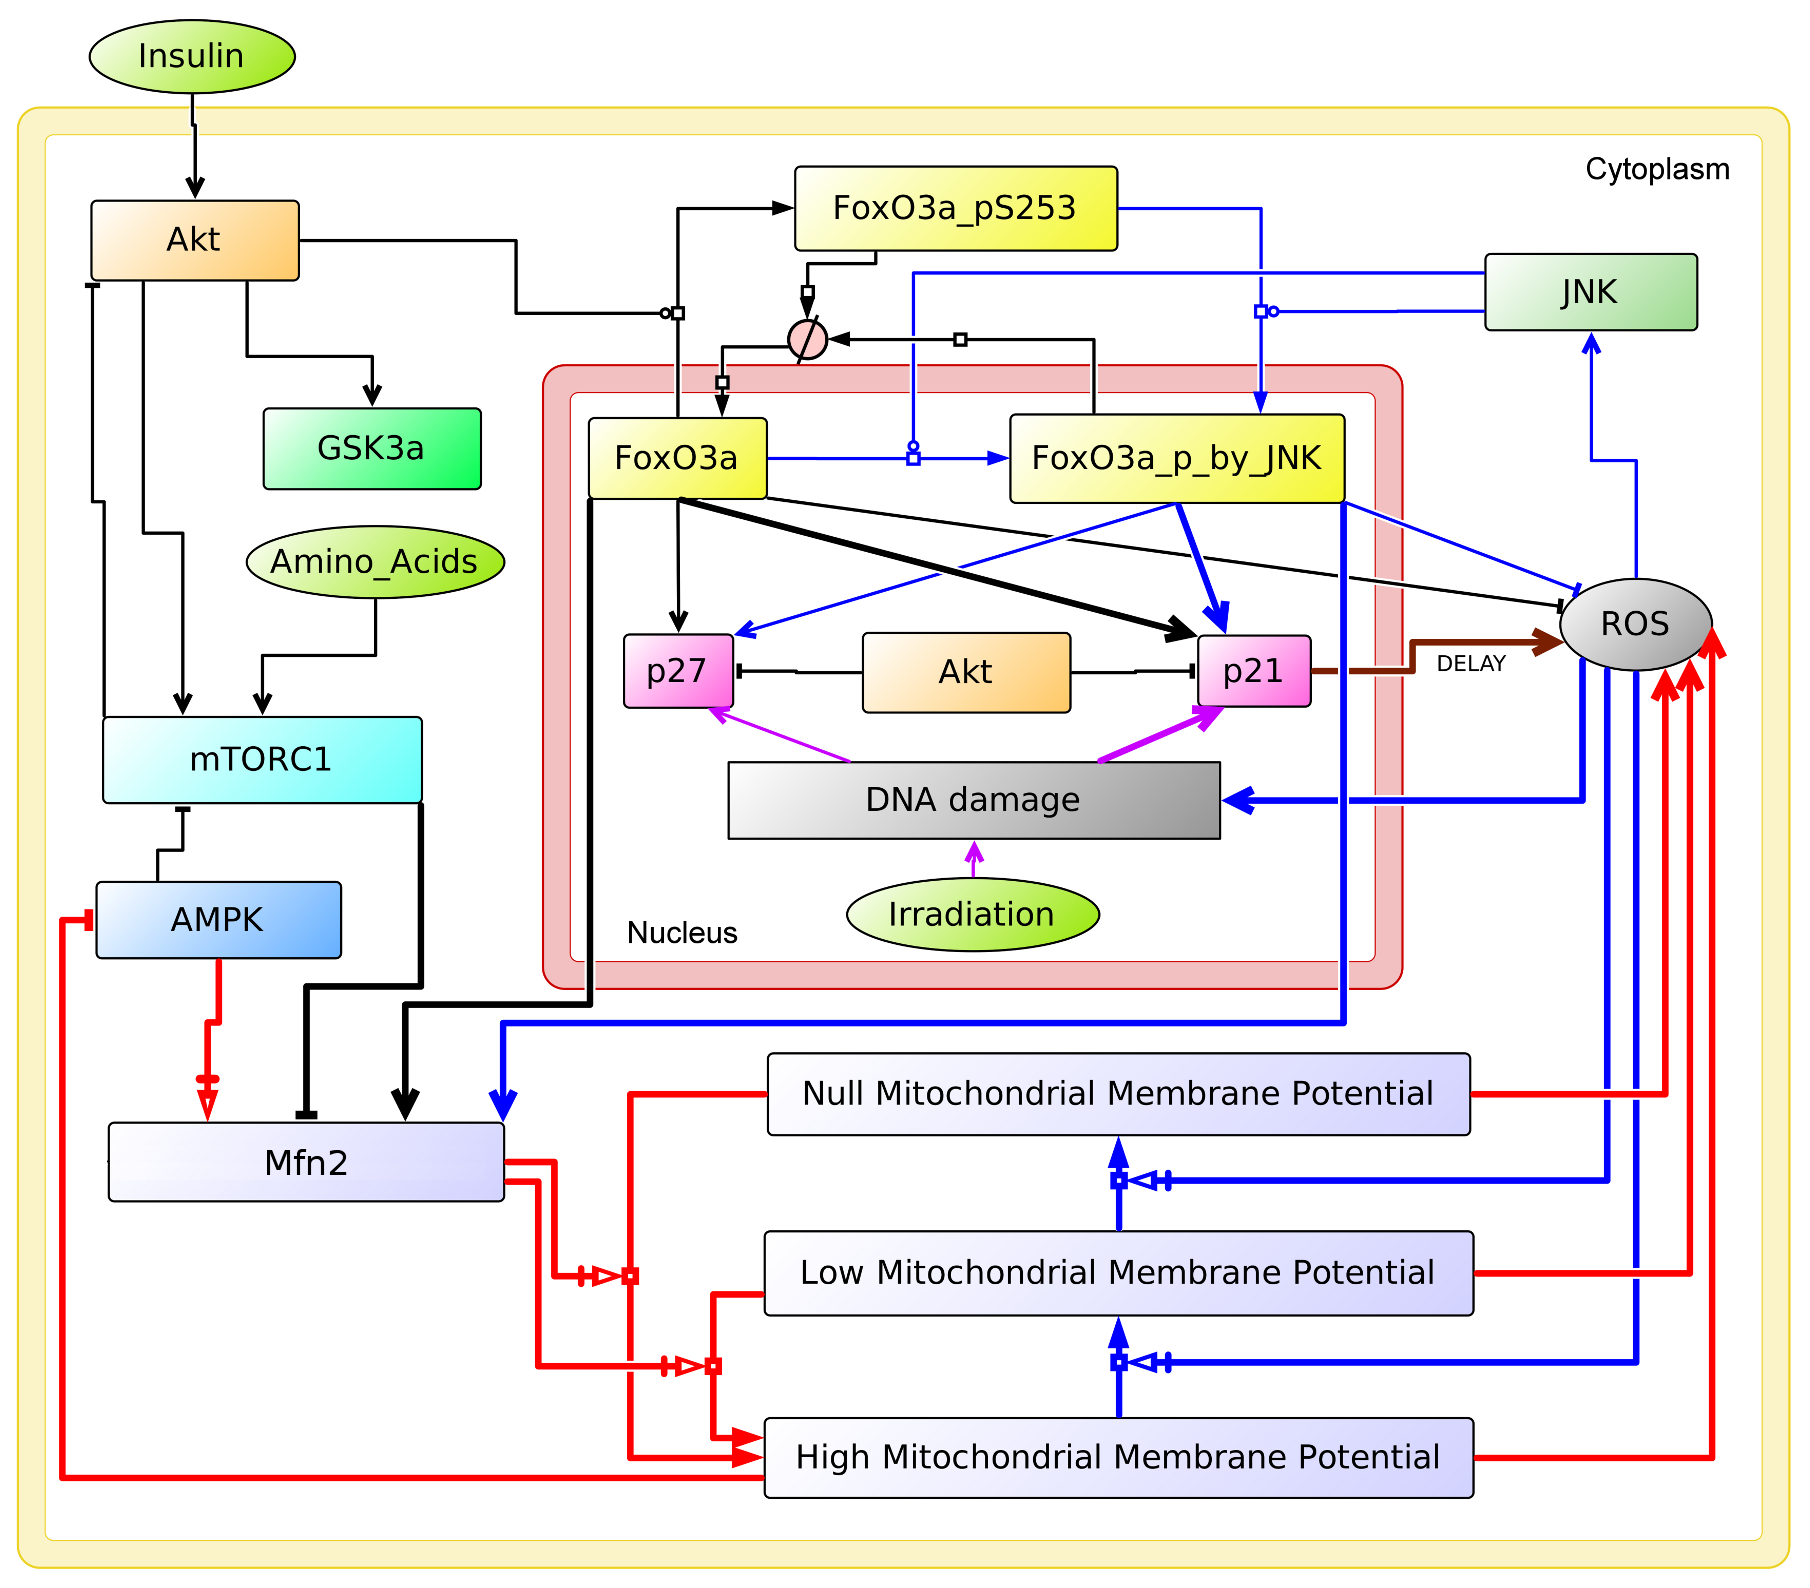
\includegraphics[width=5.4in]{senescence_model.png}
		\caption[A dynamical model for irradiation-induced cellular senescence]{A dynamical model for irradiation-induced cellular senescence. Graphical model integrating the insulin-TOR (IIS-TOR) signalling pathway (left, black reactions), the oxidative stress response (right, blue reactions), FoxO3a regulation (top), nuclear DNA damage (centre, magenta reaction) and mitochondrial phenotype (bottom, red reactions).}
		\label{fig:project3_senescence_model}
	\end{center}
\end{figure}
\clearpage


\begin{figure}[tb]
	\begin{center}
		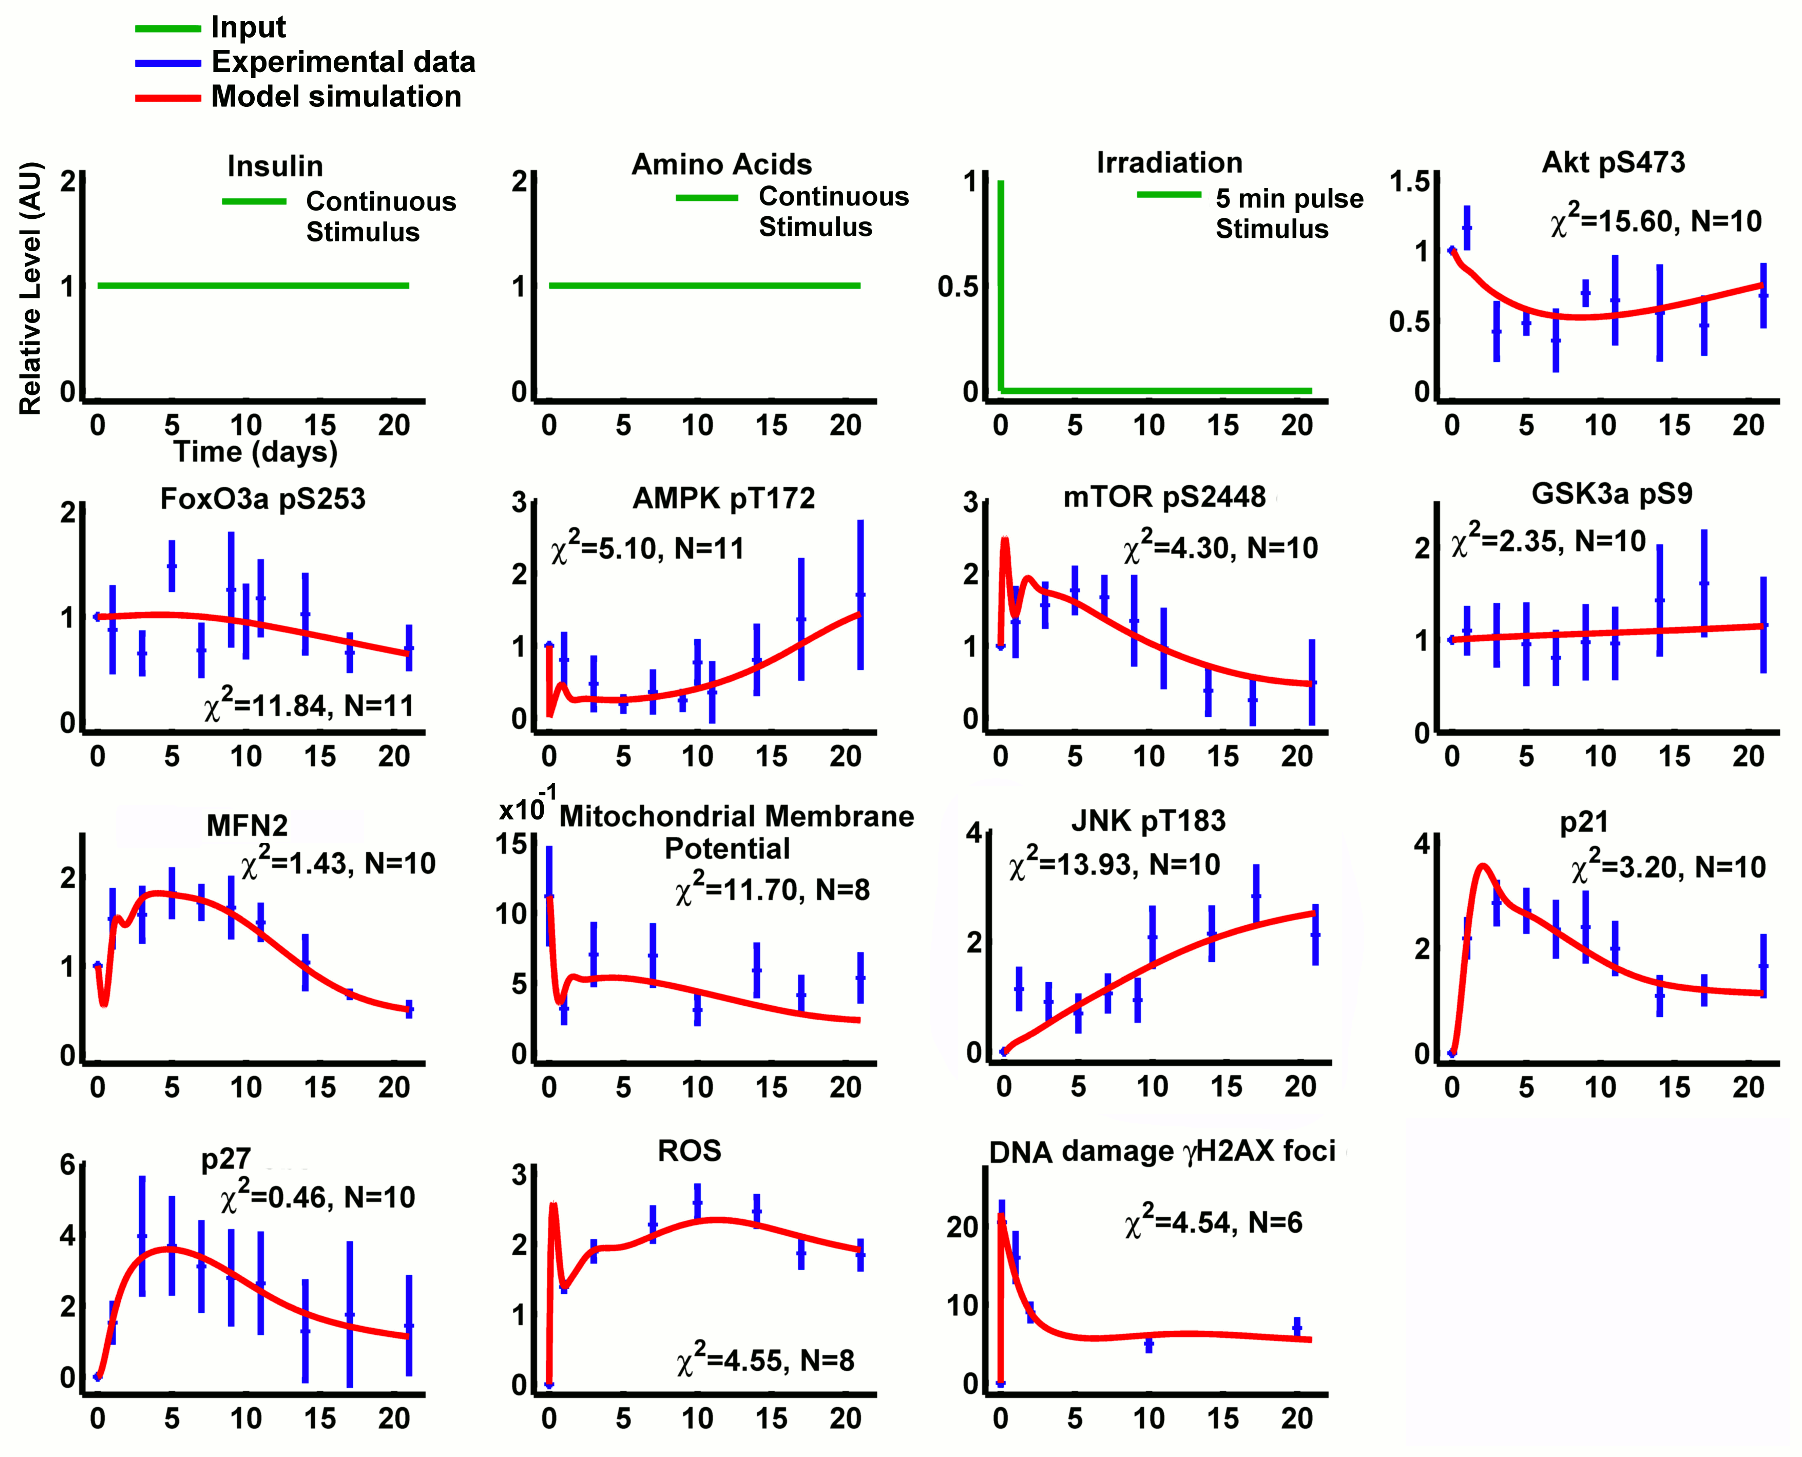
\includegraphics[width=5.0in]{senescence_model_timecourses.png}
		\caption[\emph{In silico} versus \emph{in vitro} time courses]{\emph{In silico} versus \emph{in vitro} time courses. The model (red lines) was calibrated over experimental time course data (see blue points) collected for 13 readouts in the network up to 21 days. The inputs are amino acids/insulin (constant inputs) and irradiation (pulse input of 5 min which simulates 20 Gy X ray irradiation over 5 min). Experimental time points (blue points) are mean +/- 1 standard deviation collected from 5 repetitions. \emph{In vitro} experiments were performed by Dr Glyn Nelson, Newcastle University, UK.}
		\label{fig:project3_senescence_model_timecourses}
	\end{center}
\end{figure}
\clearpage


\begin{figure}[tb]
	\begin{center}
		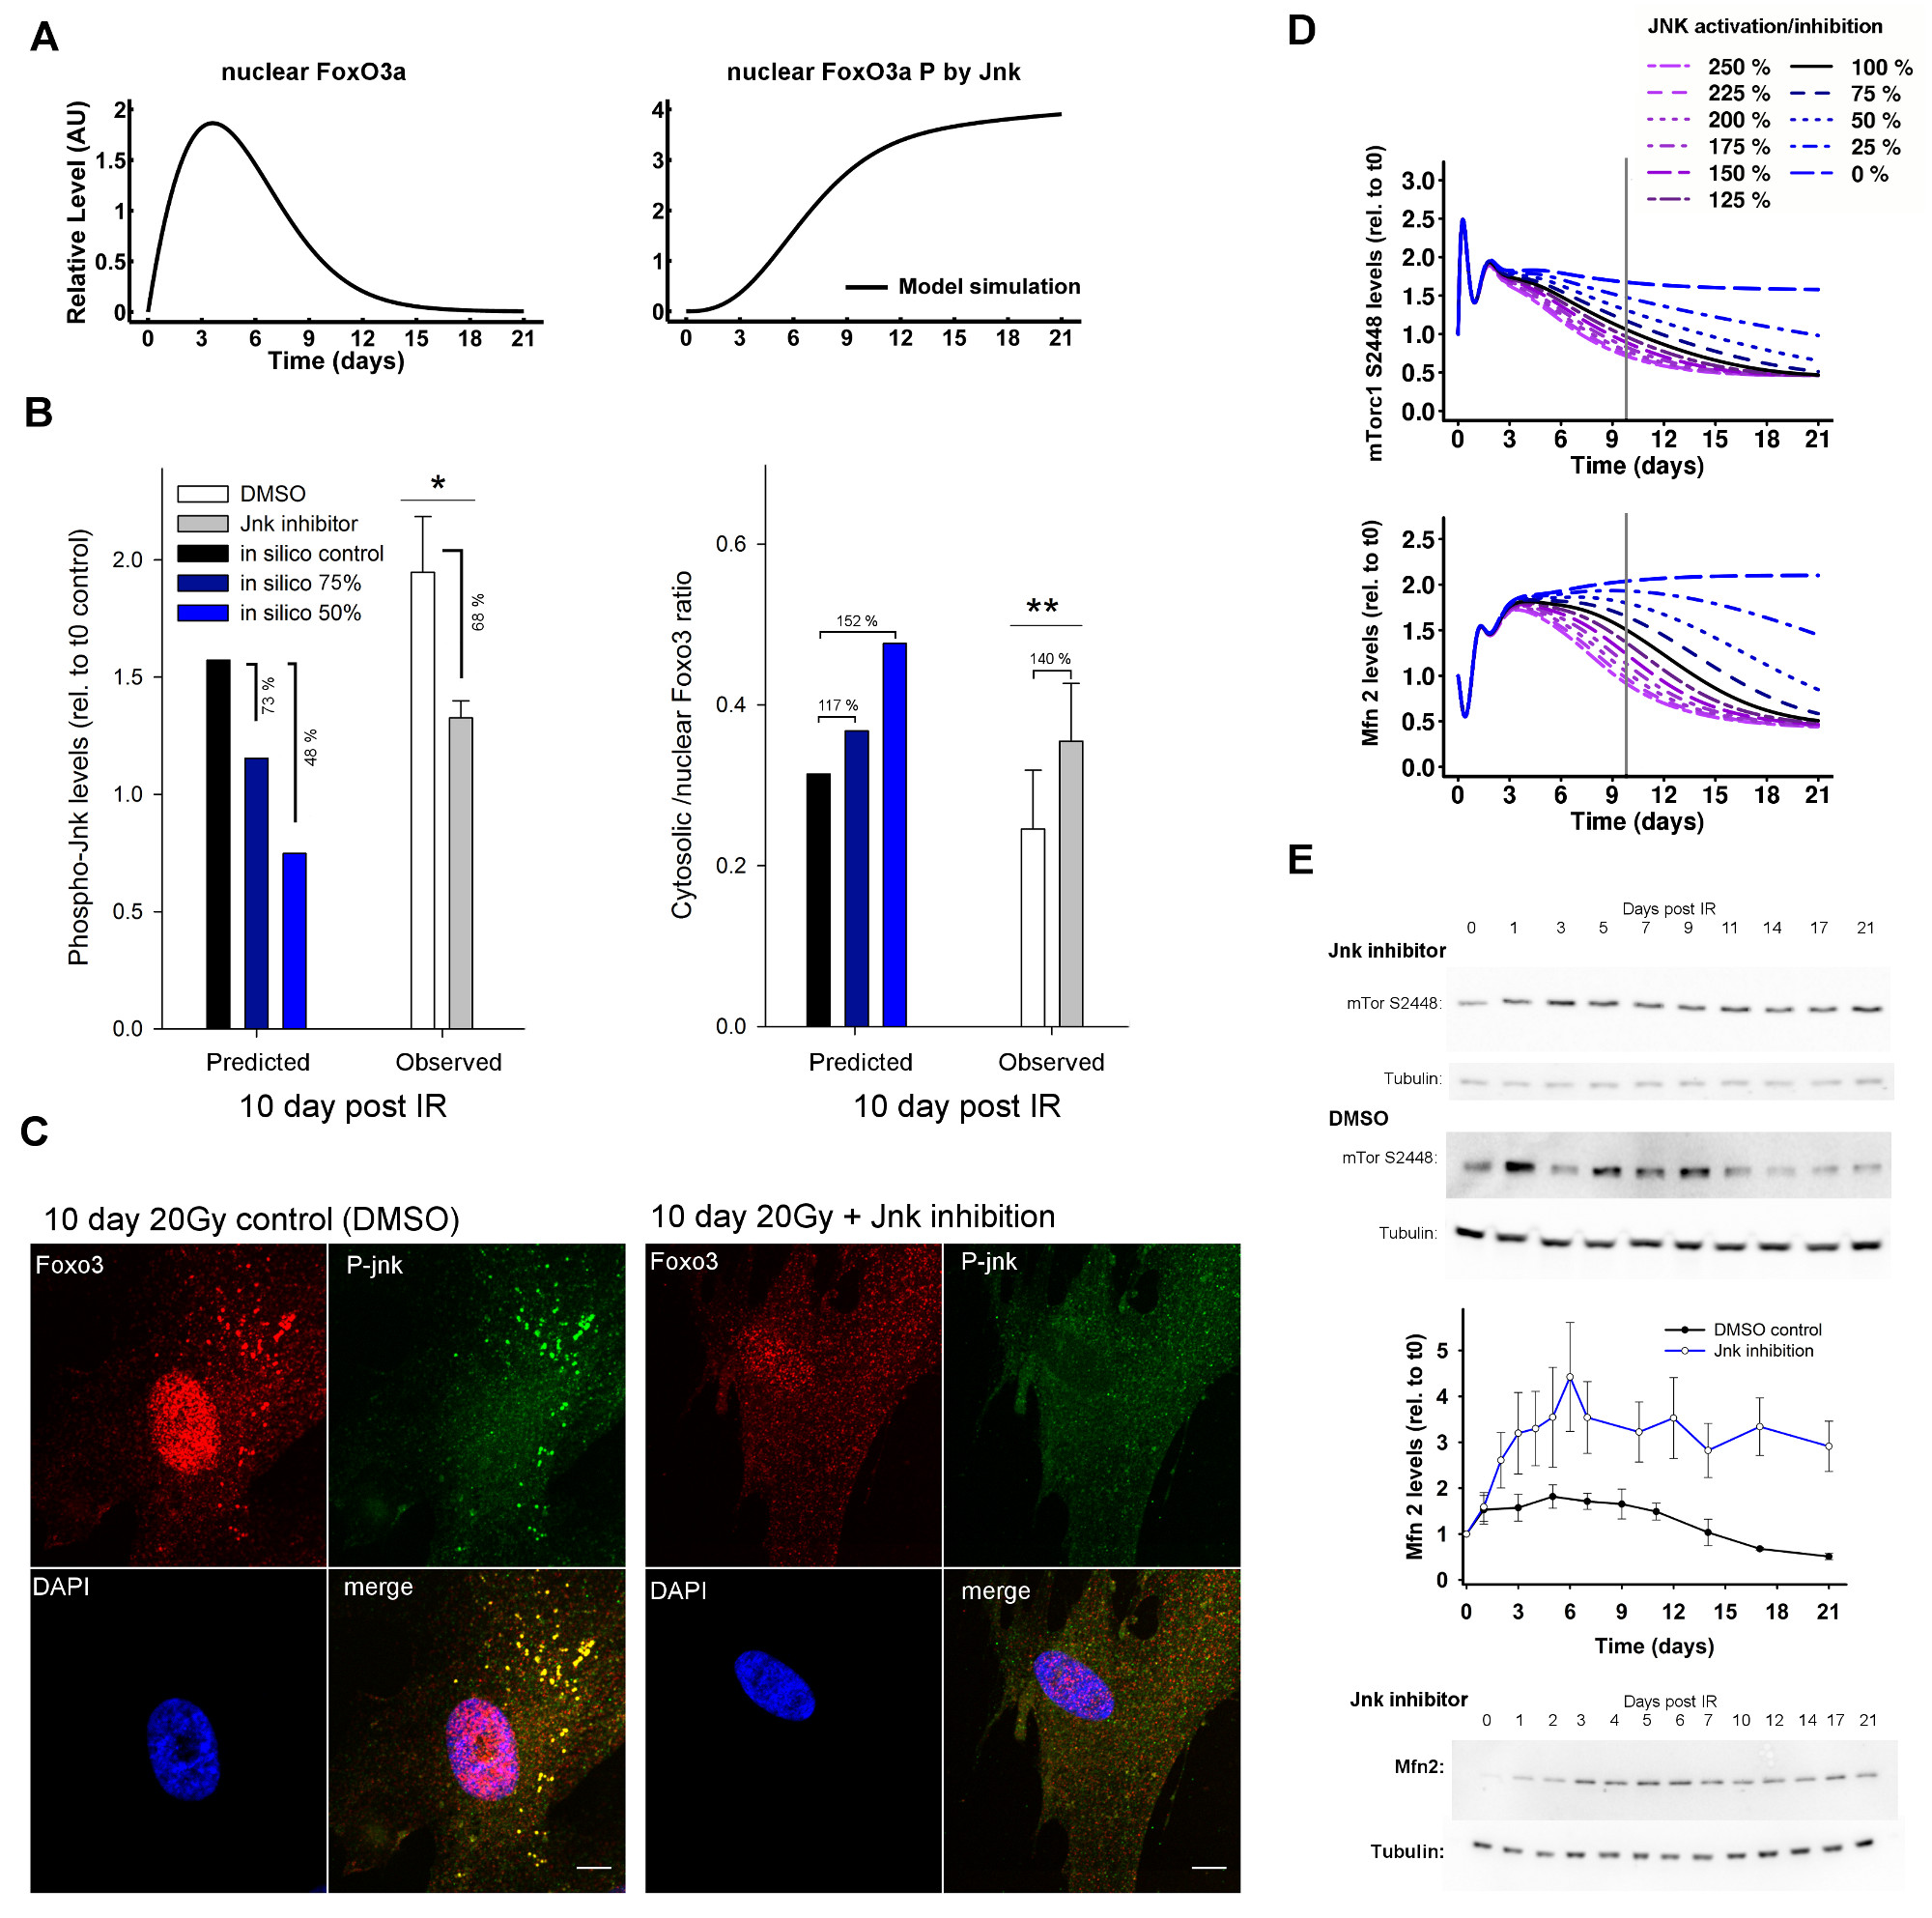
\includegraphics[width=5.8in]{fig2_121029b.jpg}
		\caption[JNK inhibition promotes cytoplasmic FoxO3a migration and Mfn2]{JNK inhibition promotes cytoplasmic FoxO3a migration and Mfn2. (A) \emph{In silico} time-courses for nuclear unphosphorylated FoxO3a and JNK-phosphorylated FoxO3a showing a shift towards active FoxO3a being predominantly phosphorylated by JNK over time after stress induced premature senescence. (B) At 10 days post irradiation, the model quantitatively predicted a decrease in total phosphorylated JNK and an increase in cytosolic fraction of FoxO3a upon JNK inhibition (black and blue histograms). These predictions were confirmed \emph{in vitro}. MRC5 cells were irradiated to cause stress-induced senescence then incubated with a JNK inhibitor (1$\mu$M SP600125). 10 days post irradiation, cells were stained for phosphorylated JNK (T183/Y185) and total FoxO3a. Quantification of fluorescence intensities indicated a significant decrease in total phosphorylated JNK (Mann-Whitney test, * P = 0.014) and a significant increase in 
cytosolic fraction of FoxO3a (\emph{t}-test, ** P = 0.010) (white and grey histograms). (C) Example fluorescence images for the previous quantification. (D) Downstream of FoxO3a, the model predicted increases in mTORC1-pS2448 phosphorylation and mitofusin2 upregulation in a JNK-dependent manner. (E) Western blotting data confirmed the changes in mTORC1-pS2448 and mitofusin2 levels following MRC5 cells up to 21 days post irradiation in the presence of JNK inhibitor. See Figure \ref{fig:project3_collect_jnk_single_perturb} for other readouts upon \emph{in silico} JNK perturbation. \emph{In vitro} experiments (Panels B:Observed, C and E) were performed by Dr Glyn Nelson, Newcastle University, UK.}
		\label{fig:project3_fig2_121029b}
	\end{center}
\end{figure}
\clearpage

\begin{figure}[tb]
	\begin{center}
		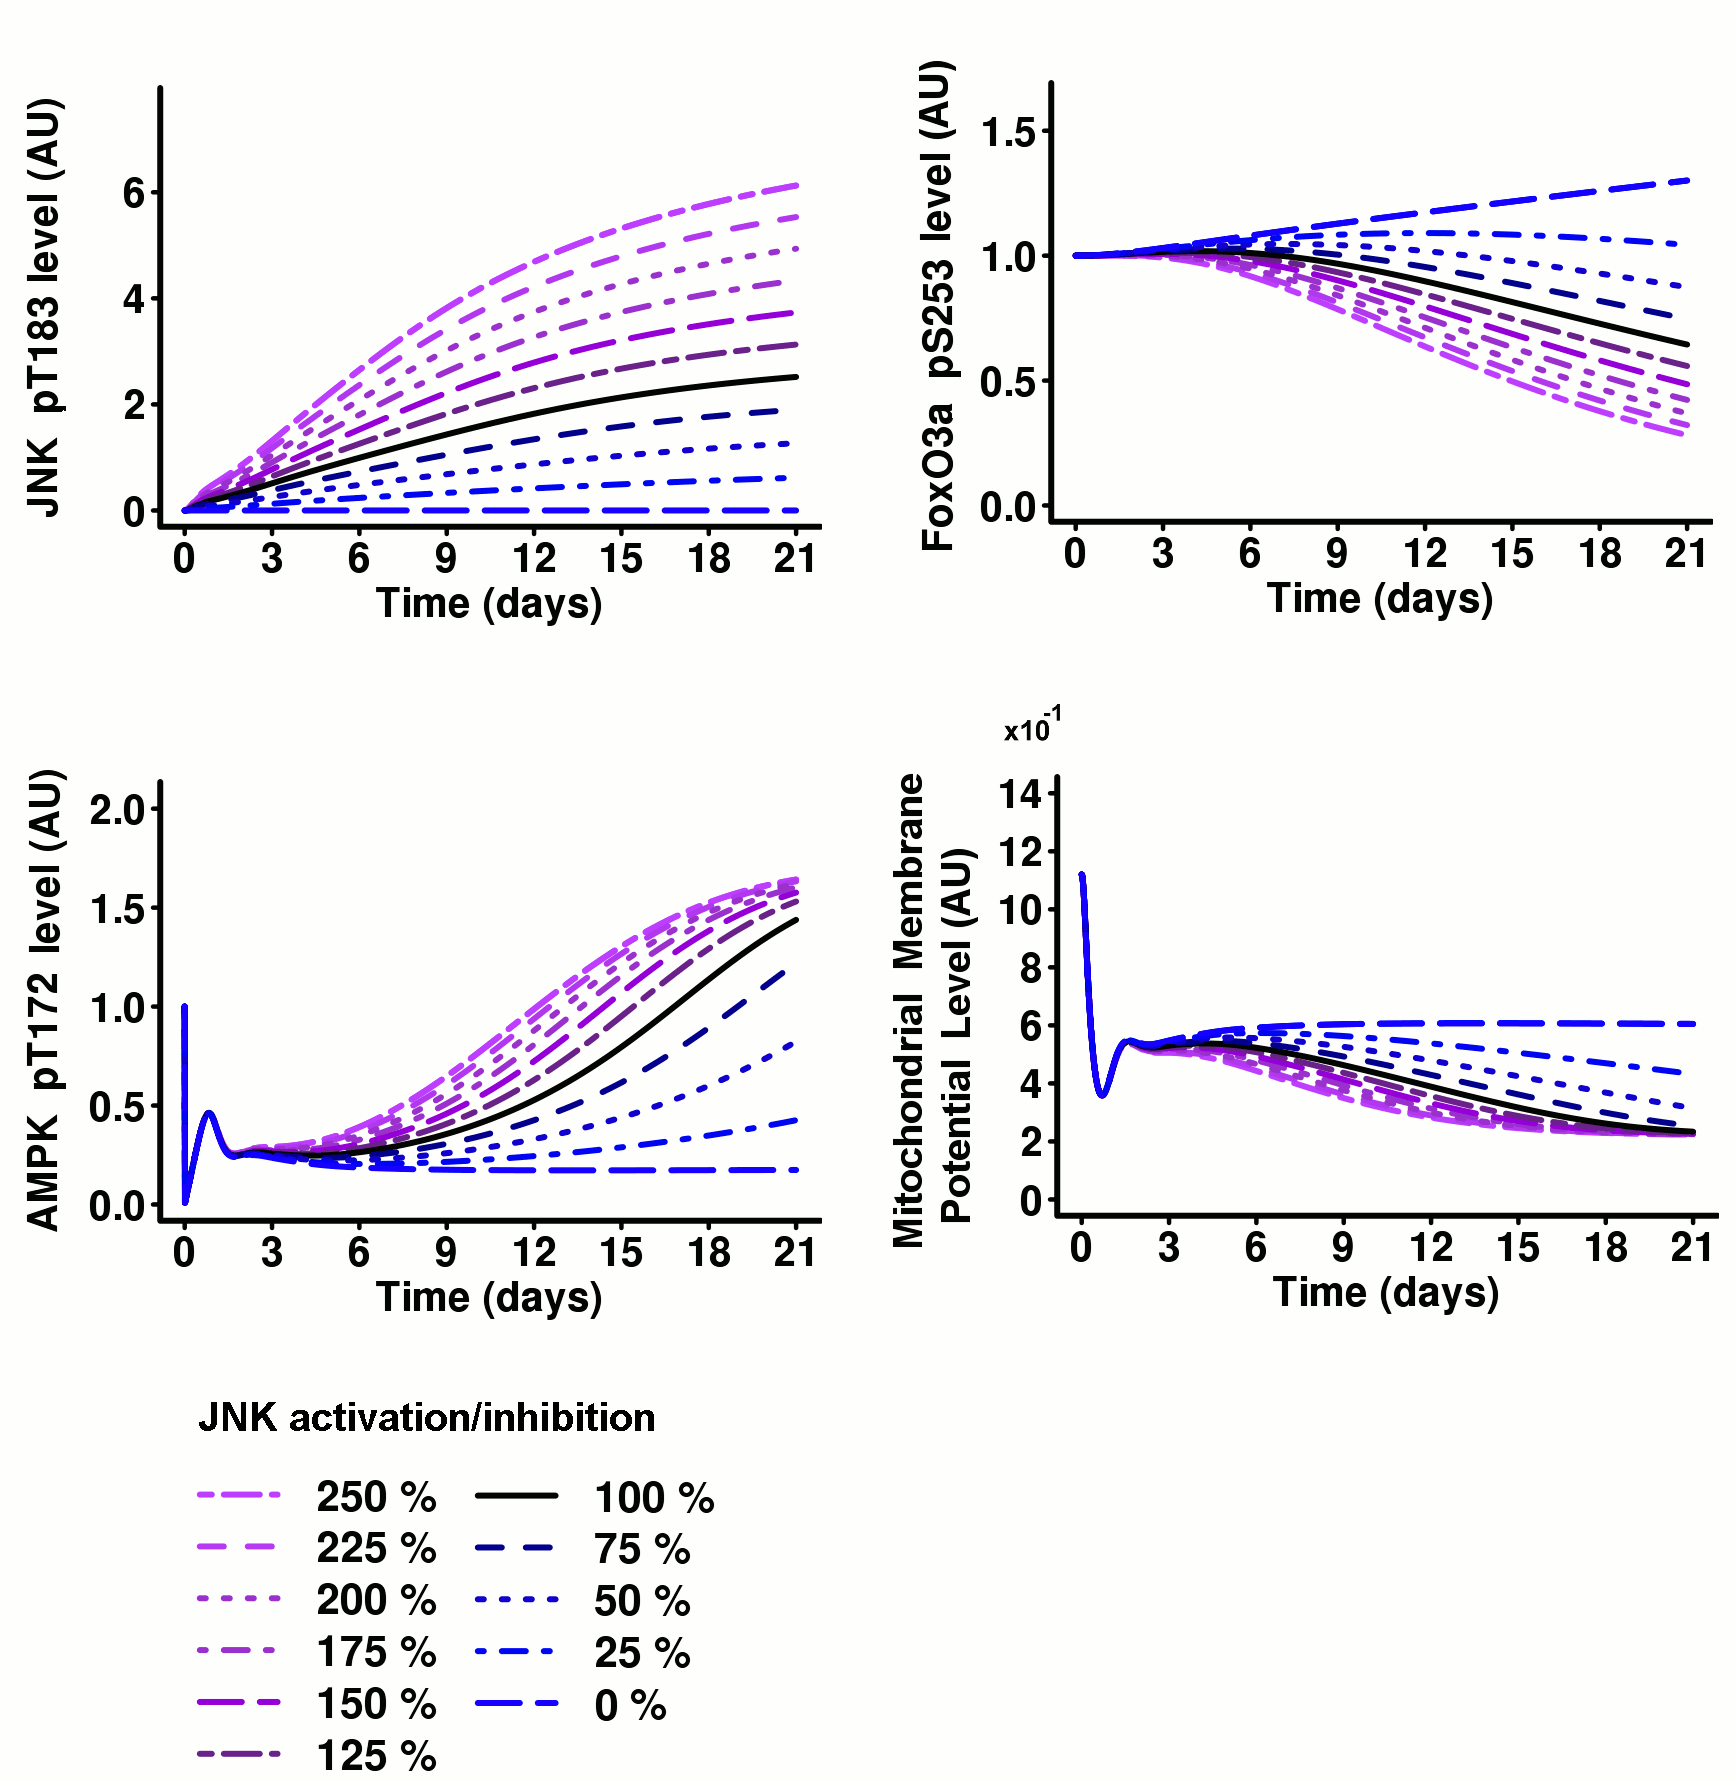
\includegraphics[width=4in]{collect_jnk_single_perturb.png}
		\caption[Other simulated readouts for JNK single perturbation]{Other simulated readouts for JNK single perturbation. After 6-9 days post irradiation, the levels of AMPK dramatically decreased in a JNK inhibition treatment. Conversely, the mitochondrial membrane potential increased although its level did not recover to levels achieved before day 3.}
		\label{fig:project3_collect_jnk_single_perturb}
	\end{center}
\end{figure}
\clearpage


\begin{figure}[tb]
	\begin{center}
		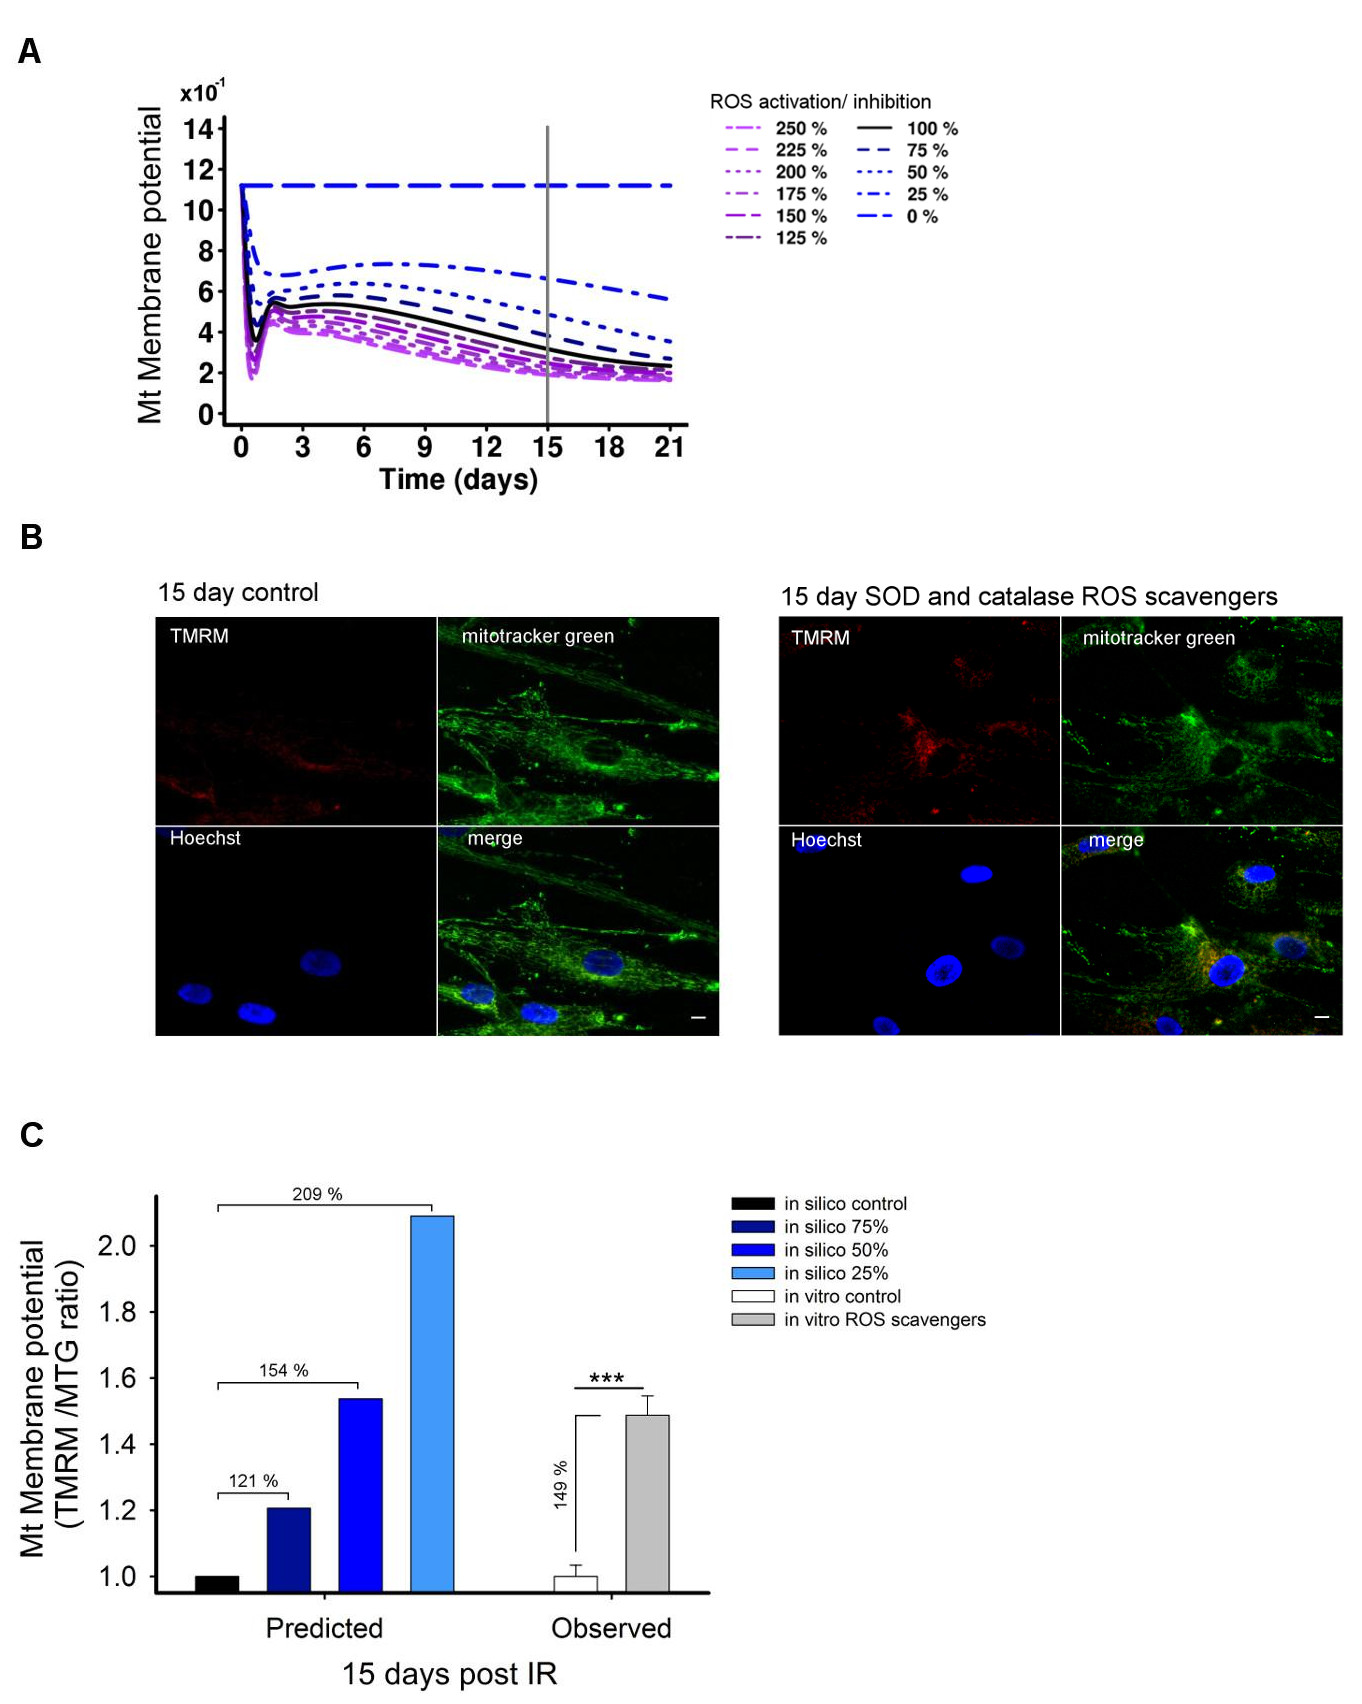
\includegraphics[width=5.0in]{fig3_121026b.jpg}
		\caption[ROS inhibition improves mitochondrial membrane potential]{ROS inhibition improves mitochondrial membrane potential. (A) At 15 days post irradiation, the model quantitatively predicted an increase in mitochondrial (mt) membrane potential upon ROS inhibition (black and blue histograms). (B) Example images of control cells (upper panel) and cells treated with SOD and catalase (100U each) in the medium (lower panel) for 15 days post IR are shown. (C) The model prediction was confirmed by quantification of the fluorescence intensities. Exogenous addition of SOD and catalase significantly increased the average membrane potential (Mann-Whitney test, *** P $<$ 0.001) \emph{in vitro}. \emph{In silico} inhibition of ROS levels also partially reactivated mt membrane potential in a dose dependent manner, with between 75 and 50\% levels giving equivalent restoration of membrane potential to the \emph{in vitro} data. \emph{In vitro} mt membrane potential was determined in MRC5 cells 15 days post IR using live 
cell imaging of cells loaded with the mt membrane potential dependent dye TMRM, non-potential dependent mitotracker green and nuclear counterstain Hoechst 33342. Scale bar is 10 $\mu$m. See Figure \ref{fig:project3_collect_ros_single_perturb} for other readouts upon \emph{in silico} ROS perturbation. \emph{In vitro} experiments (Panels B, C:Observed) were performed by Dr Glyn Nelson, Newcastle University, UK.}
		\label{fig:project3_fig3_121026b}
	\end{center}
\end{figure}
\clearpage

\begin{figure}[tb]
	\begin{center}
		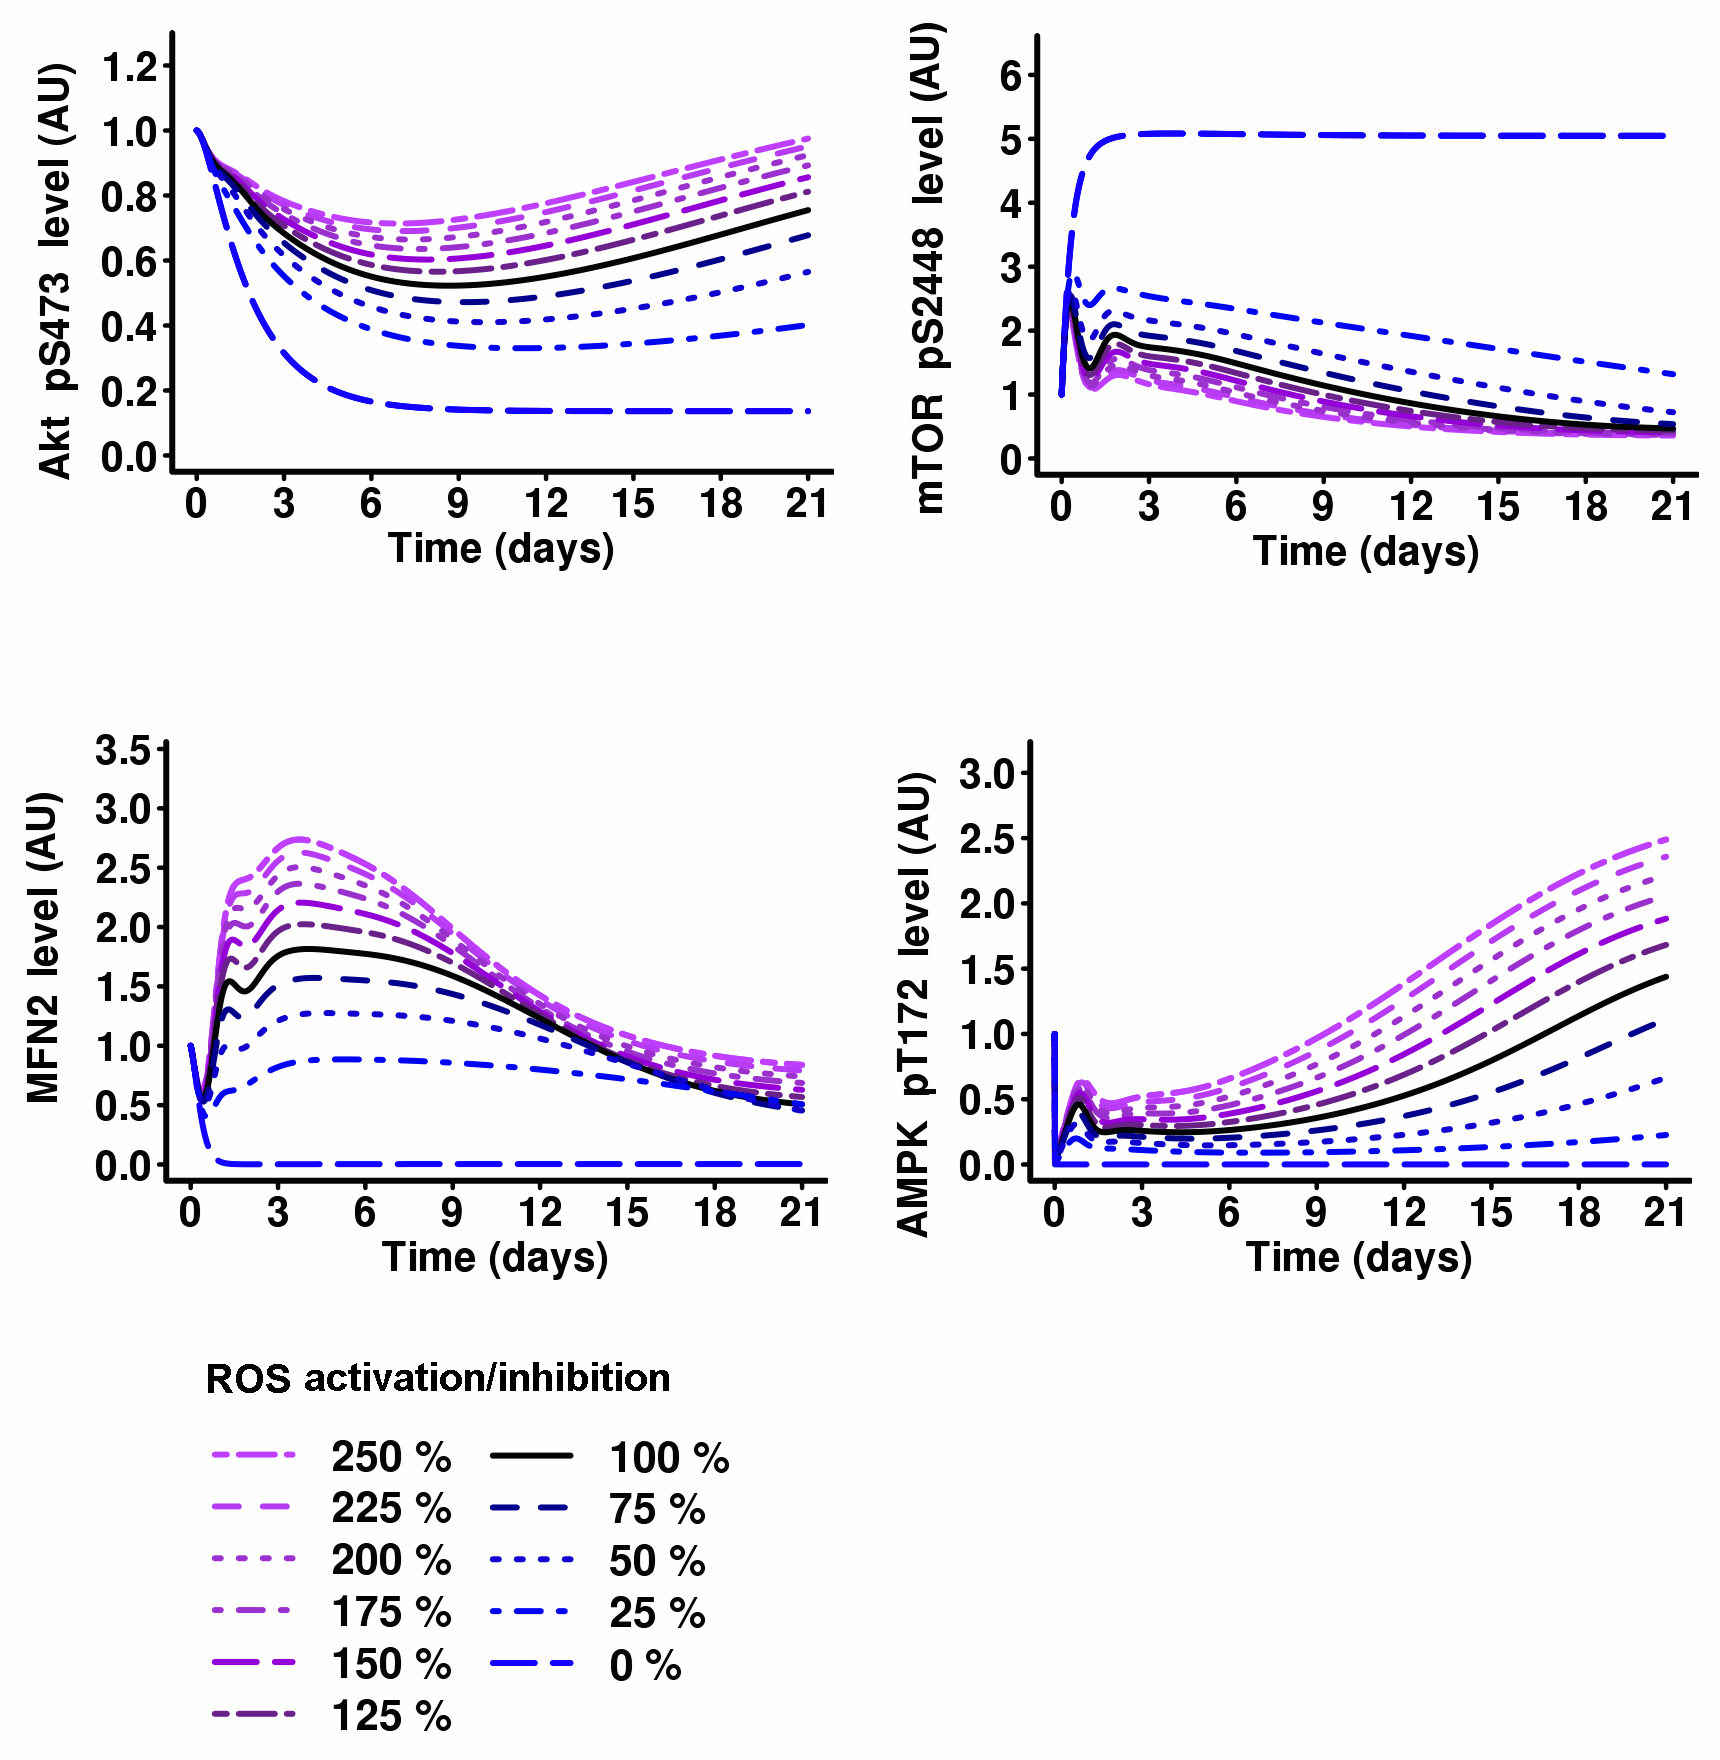
\includegraphics[width=4in]{collect_ros_single_perturb.png}
		\caption[Other simulated readouts for ROS single perturbation]{Other simulated readouts for ROS single perturbation. Upon ROS perturbation, the insulin/TOR pathway was severely affected. In details, mTOR-pS2448 levels were increased, whereas AMPK-pT172 were decreased. The reduction in mTOR-pS2448 led to an intensified mTORC1-p70-S6K-dependent negative feedback loop, reducing Akt-pS473 levels. Contrary to mTOR and AMPK dynamics, the levels of Mfn2 decreased. In addition, the system strongly lost sensitivity after day 9-11 post irradiation. This prediction meant that a ROS inhibition treatment alone is not expected to reverse senescence, especially after 9-11 days post irradiation.}
		\label{fig:project3_collect_ros_single_perturb}
	\end{center}
\end{figure}
\clearpage

\begin{figure}[tb]
	\begin{center}
		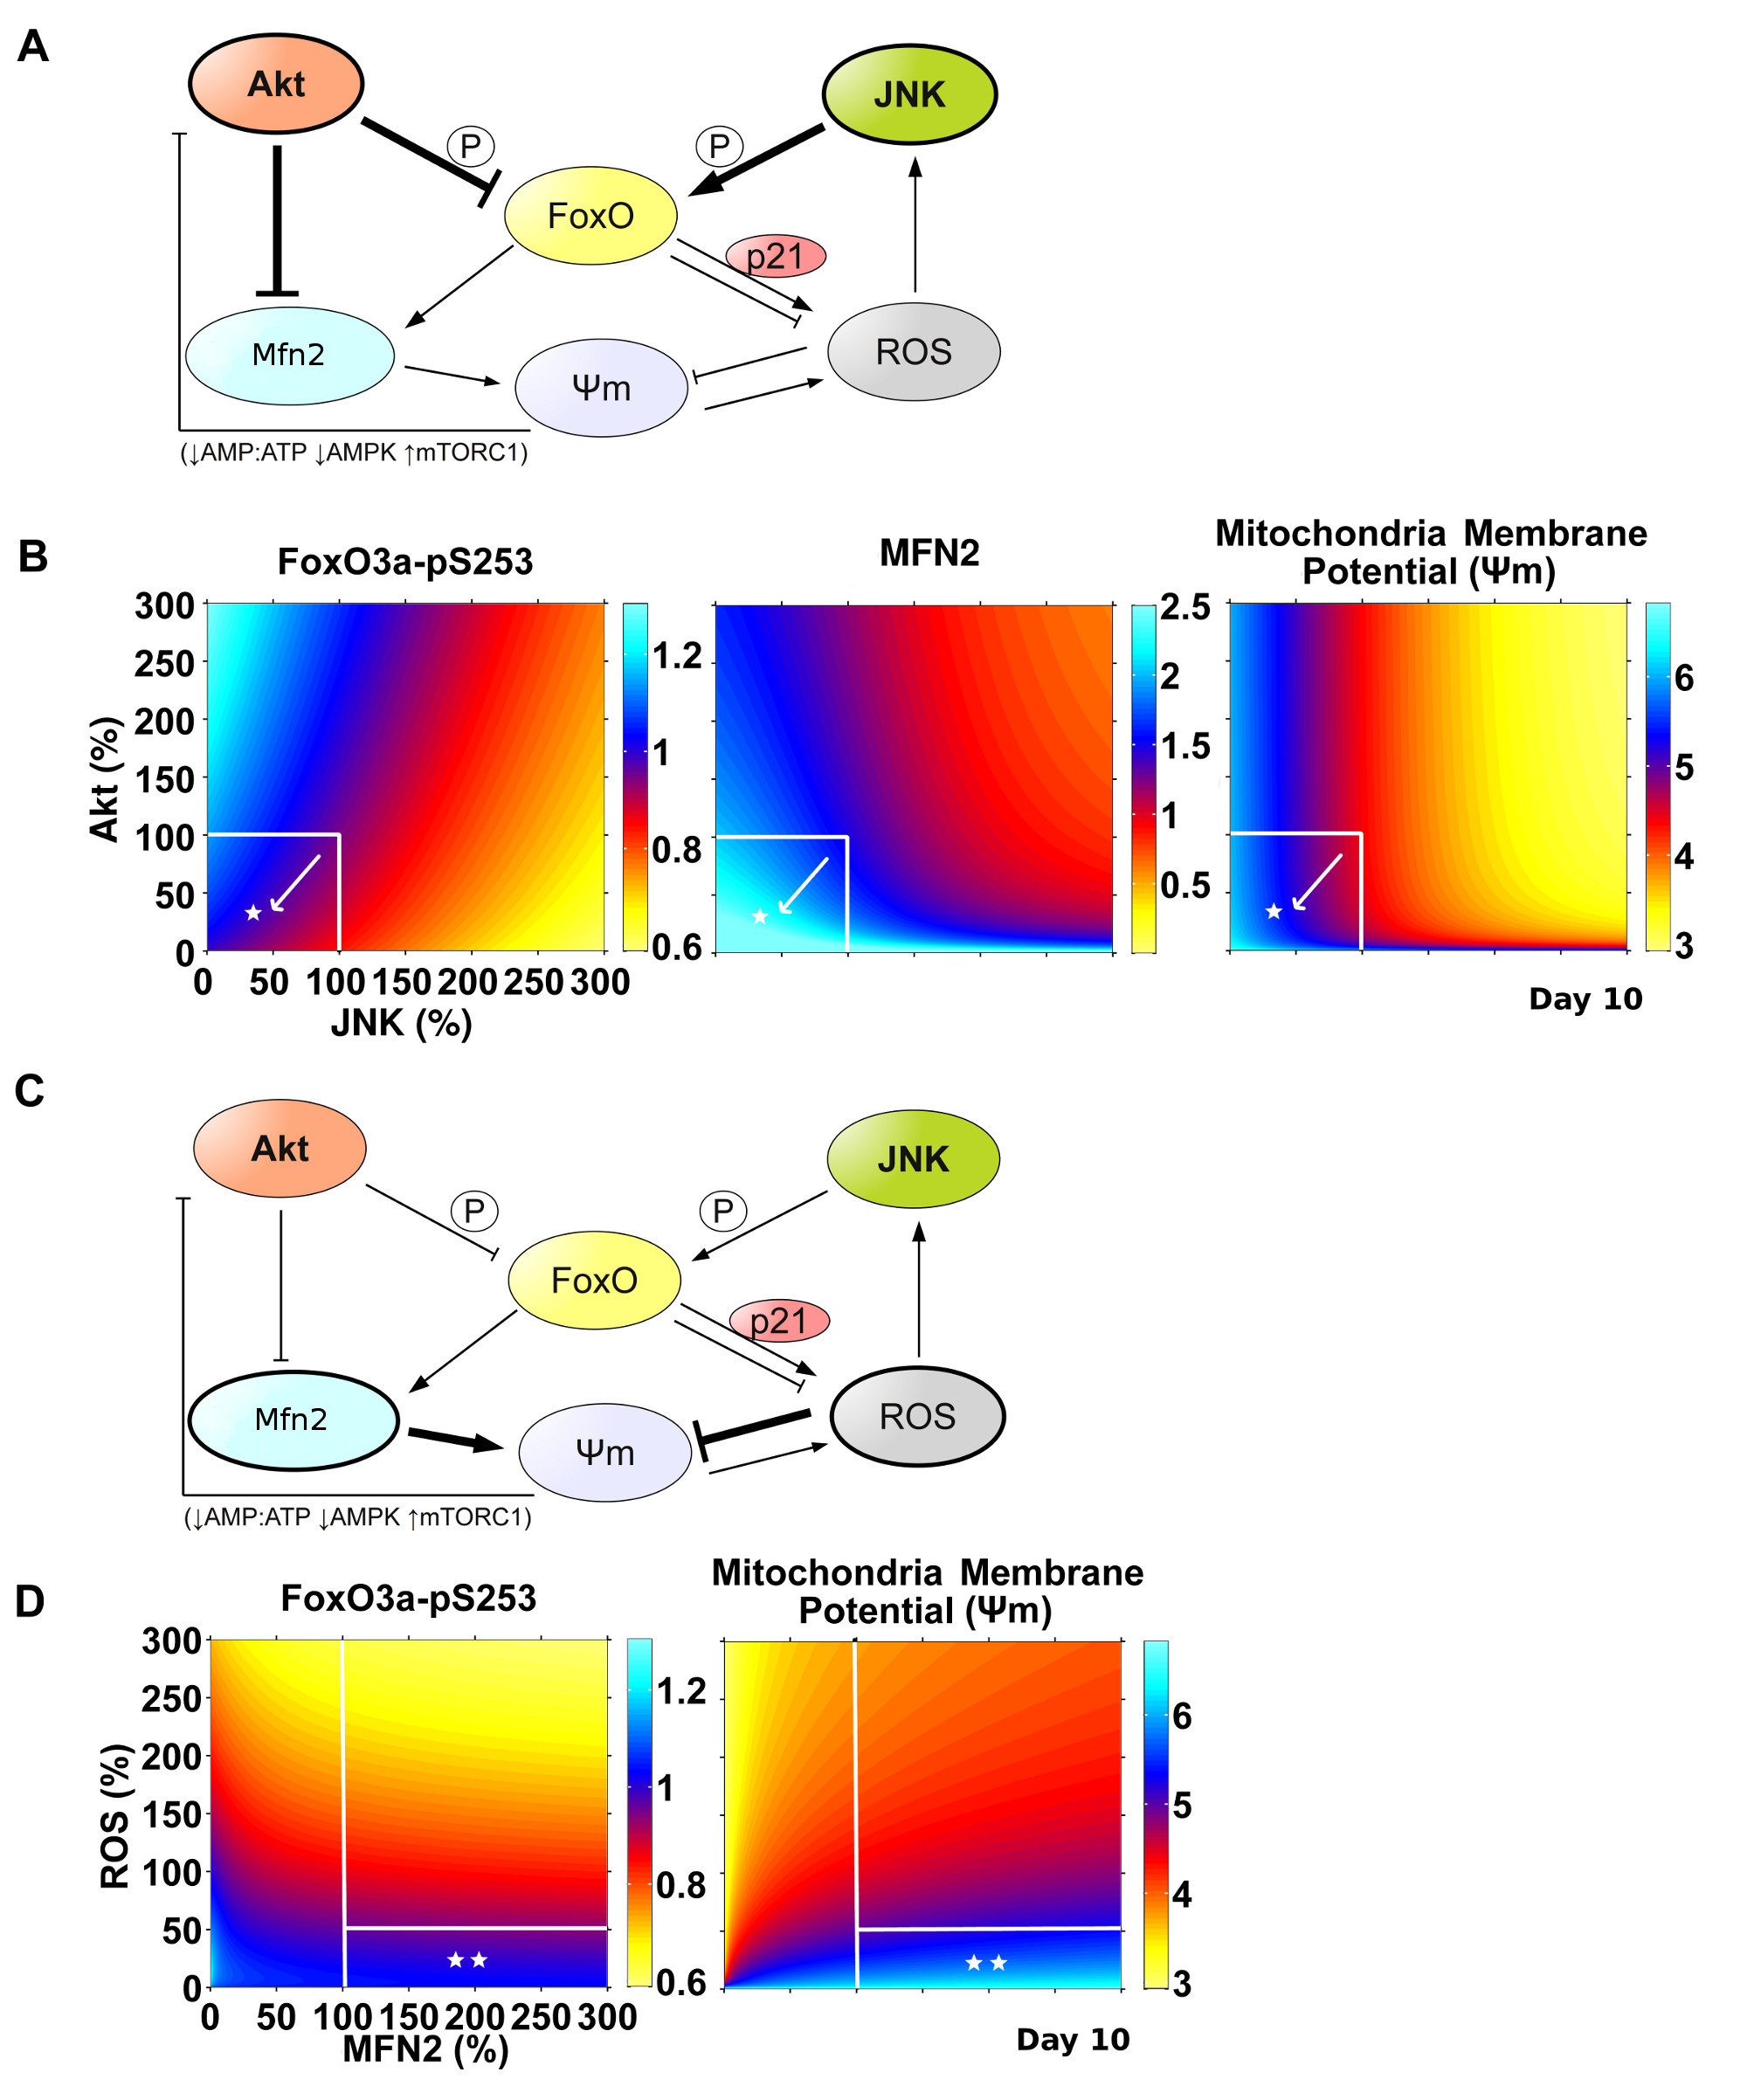
\includegraphics[width=4.5in]{figure4_121026b_inv.jpg}
		\caption[Predicted outcomes for double perturbations of JNK-Akt and Mfn2-ROS]{Predicted outcomes for double perturbations of JNK-Akt and Mfn2-ROS. (A) Schematic model illustrating the application of a combined JNK-Akt perturbation. (B) Simulation of combined JNK-Akt perturbation applied at day 0. To limit cytoplasmic FoxO3a-pS253 and to maintain JNK inhibition positive effects, intervention on cytoplasmic FoxO3a-pS253 was applied only on the \emph{inhibition region} (white square, *). Accordingly with this, Mfn2 levels and mitochondrial (mt) membrane potential increased at day 10 post irradiation. (C) Schematic model illustrating the application of a combined Mfn2-ROS perturbation. (D) Simulation of combined Mfn2-ROS perturbation applied at day 0. Using the prediction obtained in B, the double perturbation region could be largely limited to the area in the bottom (white square, **), characterised by high Mfn2 and low ROS levels. Consistently, in this area the mt membrane potential was maximised 
at day 10 post irradiation. From a mathematical point of view, a double perturbation represents a function in two variables and in this case the generated surface is seen from the top.}
		\label{fig:project3_figure4_121026c}
	\end{center}
\end{figure}
\clearpage

\begin{figure}[tb]
	\begin{center}
		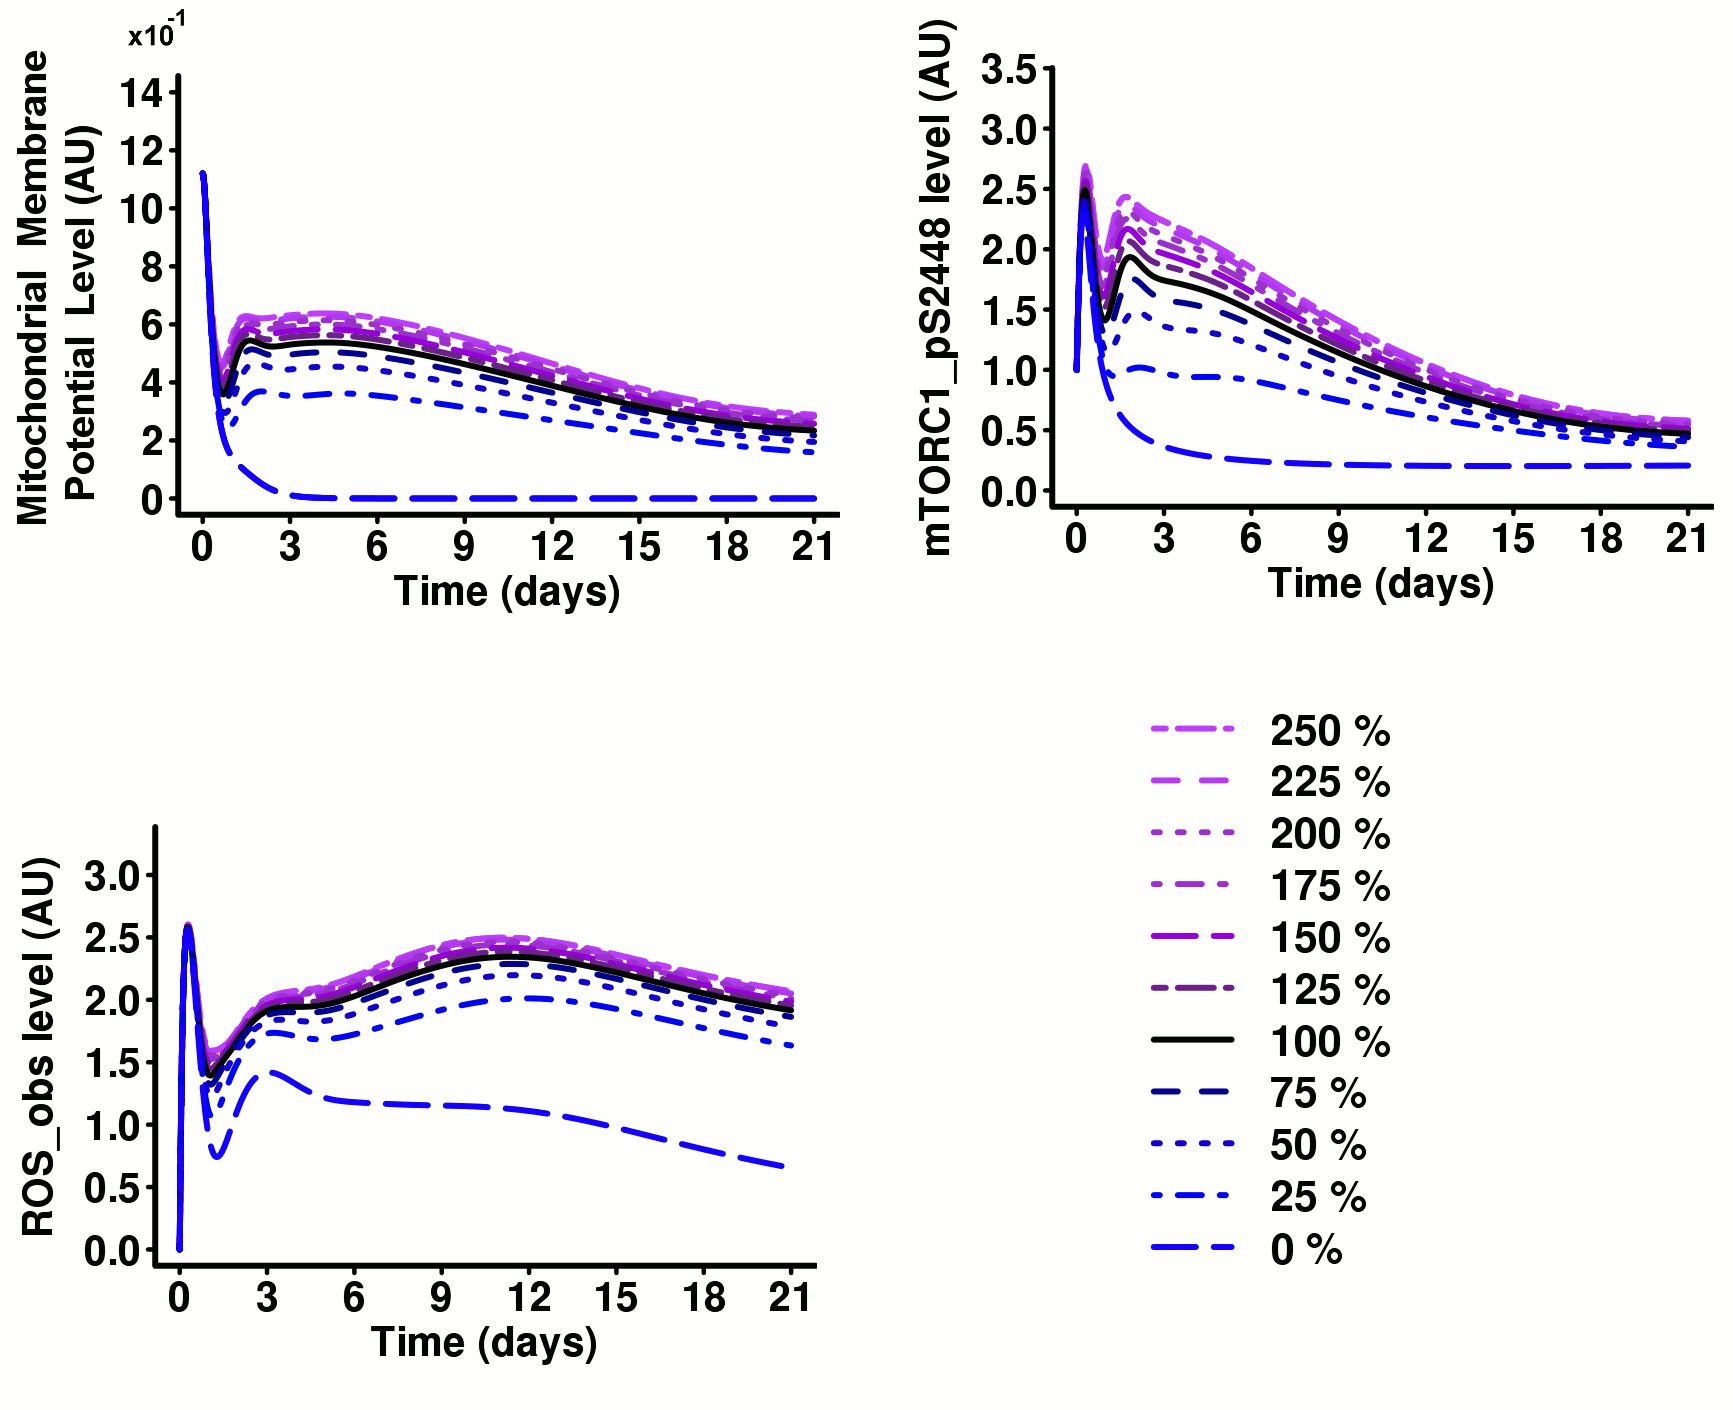
\includegraphics[width=4in]{collect_mfn2_single_perturb.png}
		\caption[Exploration of Mfn2 simulated single perturbation]{Exploration of Mfn2 simulated single perturbation. Upon a gradual inhibition of Mfn2 (blue lines), the model predicted a decrease in mitochondrial membrane potential and ROS levels. Black line indicates no perturbation of Mfn2, blue lines indicate inhibition, magenta lines indicate over-expression.}
		\label{fig:project3_collect_mfn2_single_perturb}
	\end{center}
\end{figure}
\clearpage


\begin{figure}[tb]
	\begin{center}
		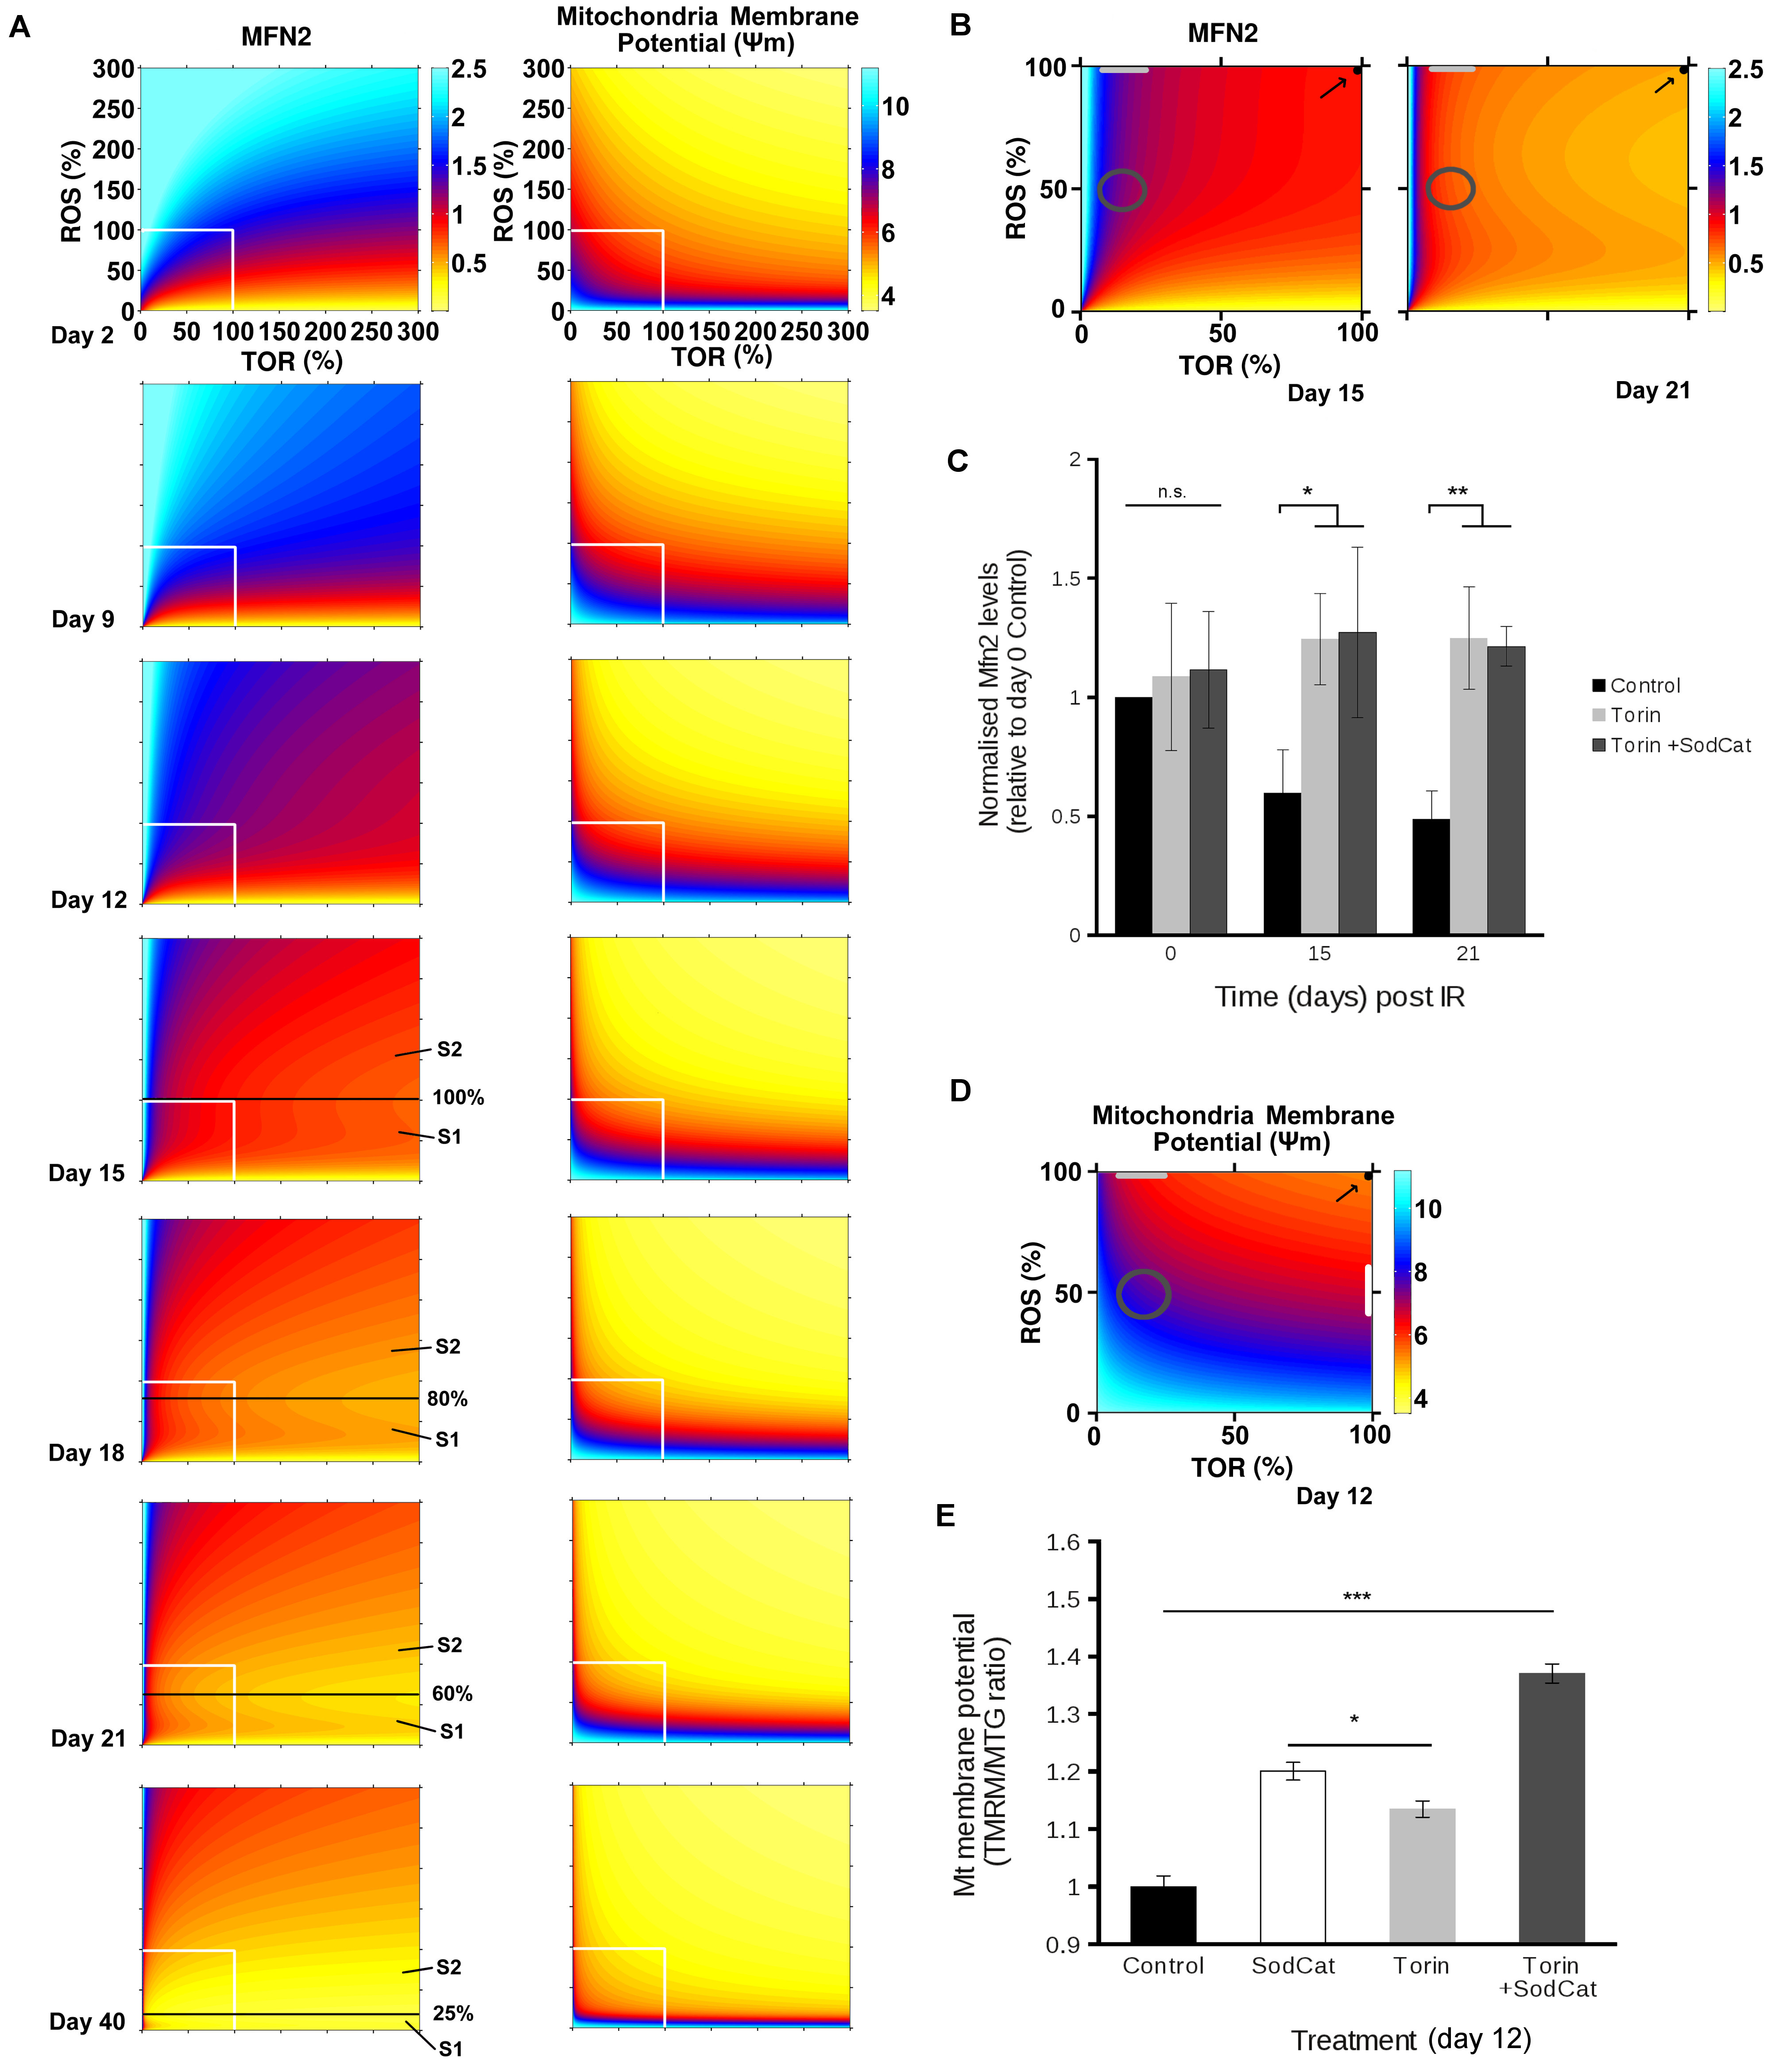
\includegraphics[width=5.4in]{figure5_121026b_inv_tested_annotated.jpg}
		\caption[Time course analysis of combined TOR-ROS perturbation]{Time course analysis of combined TOR-ROS perturbation. (A) \emph{In silico} Mfn2 and mitochondrial (mt) membrane potential time course responses upon combined TOR-ROS perturbation (0-300\% TOR or ROS level). At days 15-21, TOR and ROS perturbation split the Mfn2 response into two activation states (see $S_1$, $S_2$ divided by black line). Later, $S_1$ almost disappeared. (B) \emph{In silico} Mfn2 response upon combined TOR-ROS inhibition (0-100\% TOR or ROS level) at days 15 or 21. The black point (100\% TOR, 100\% ROS) is the control, light grey line is TOR inhibition, and dark grey circle is combined TOR-ROS inhibition. (C) \emph{In vitro} Mfn2 response upon inhibition of TOR or combined TOR-ROS at days 0, 15 or 21. Cells were treated with 20 nM Torin1 (TOR inhibitor), or Torin1 with SOD and catalase (100U each) (ANOVA with Tukey's post-hoc test, * P = 0.04, ** = 0.002, n.s. = non significant). (D) \emph{In silico} mt 
membrane potential response upon combined TOR-ROS inhibition (from 0 to 100\% TOR or ROS level) at day 12. The white line is ROS inhibition. (E) \emph{In vitro} mt membrane potential response upon inhibition of TOR, ROS or combined TOR-ROS at day 12 (ANOVA with Tukey's post-hoc test, * P = 0.028, *** P $<$ 0.001). \emph{In vitro} experiments (Panels C, E) were performed by Dr Glyn Nelson, Newcastle University, UK.}
		\label{fig:project3_figure5_121026}
	\end{center}
\end{figure}
\clearpage


\begin{figure}[tb]
	\begin{center}
		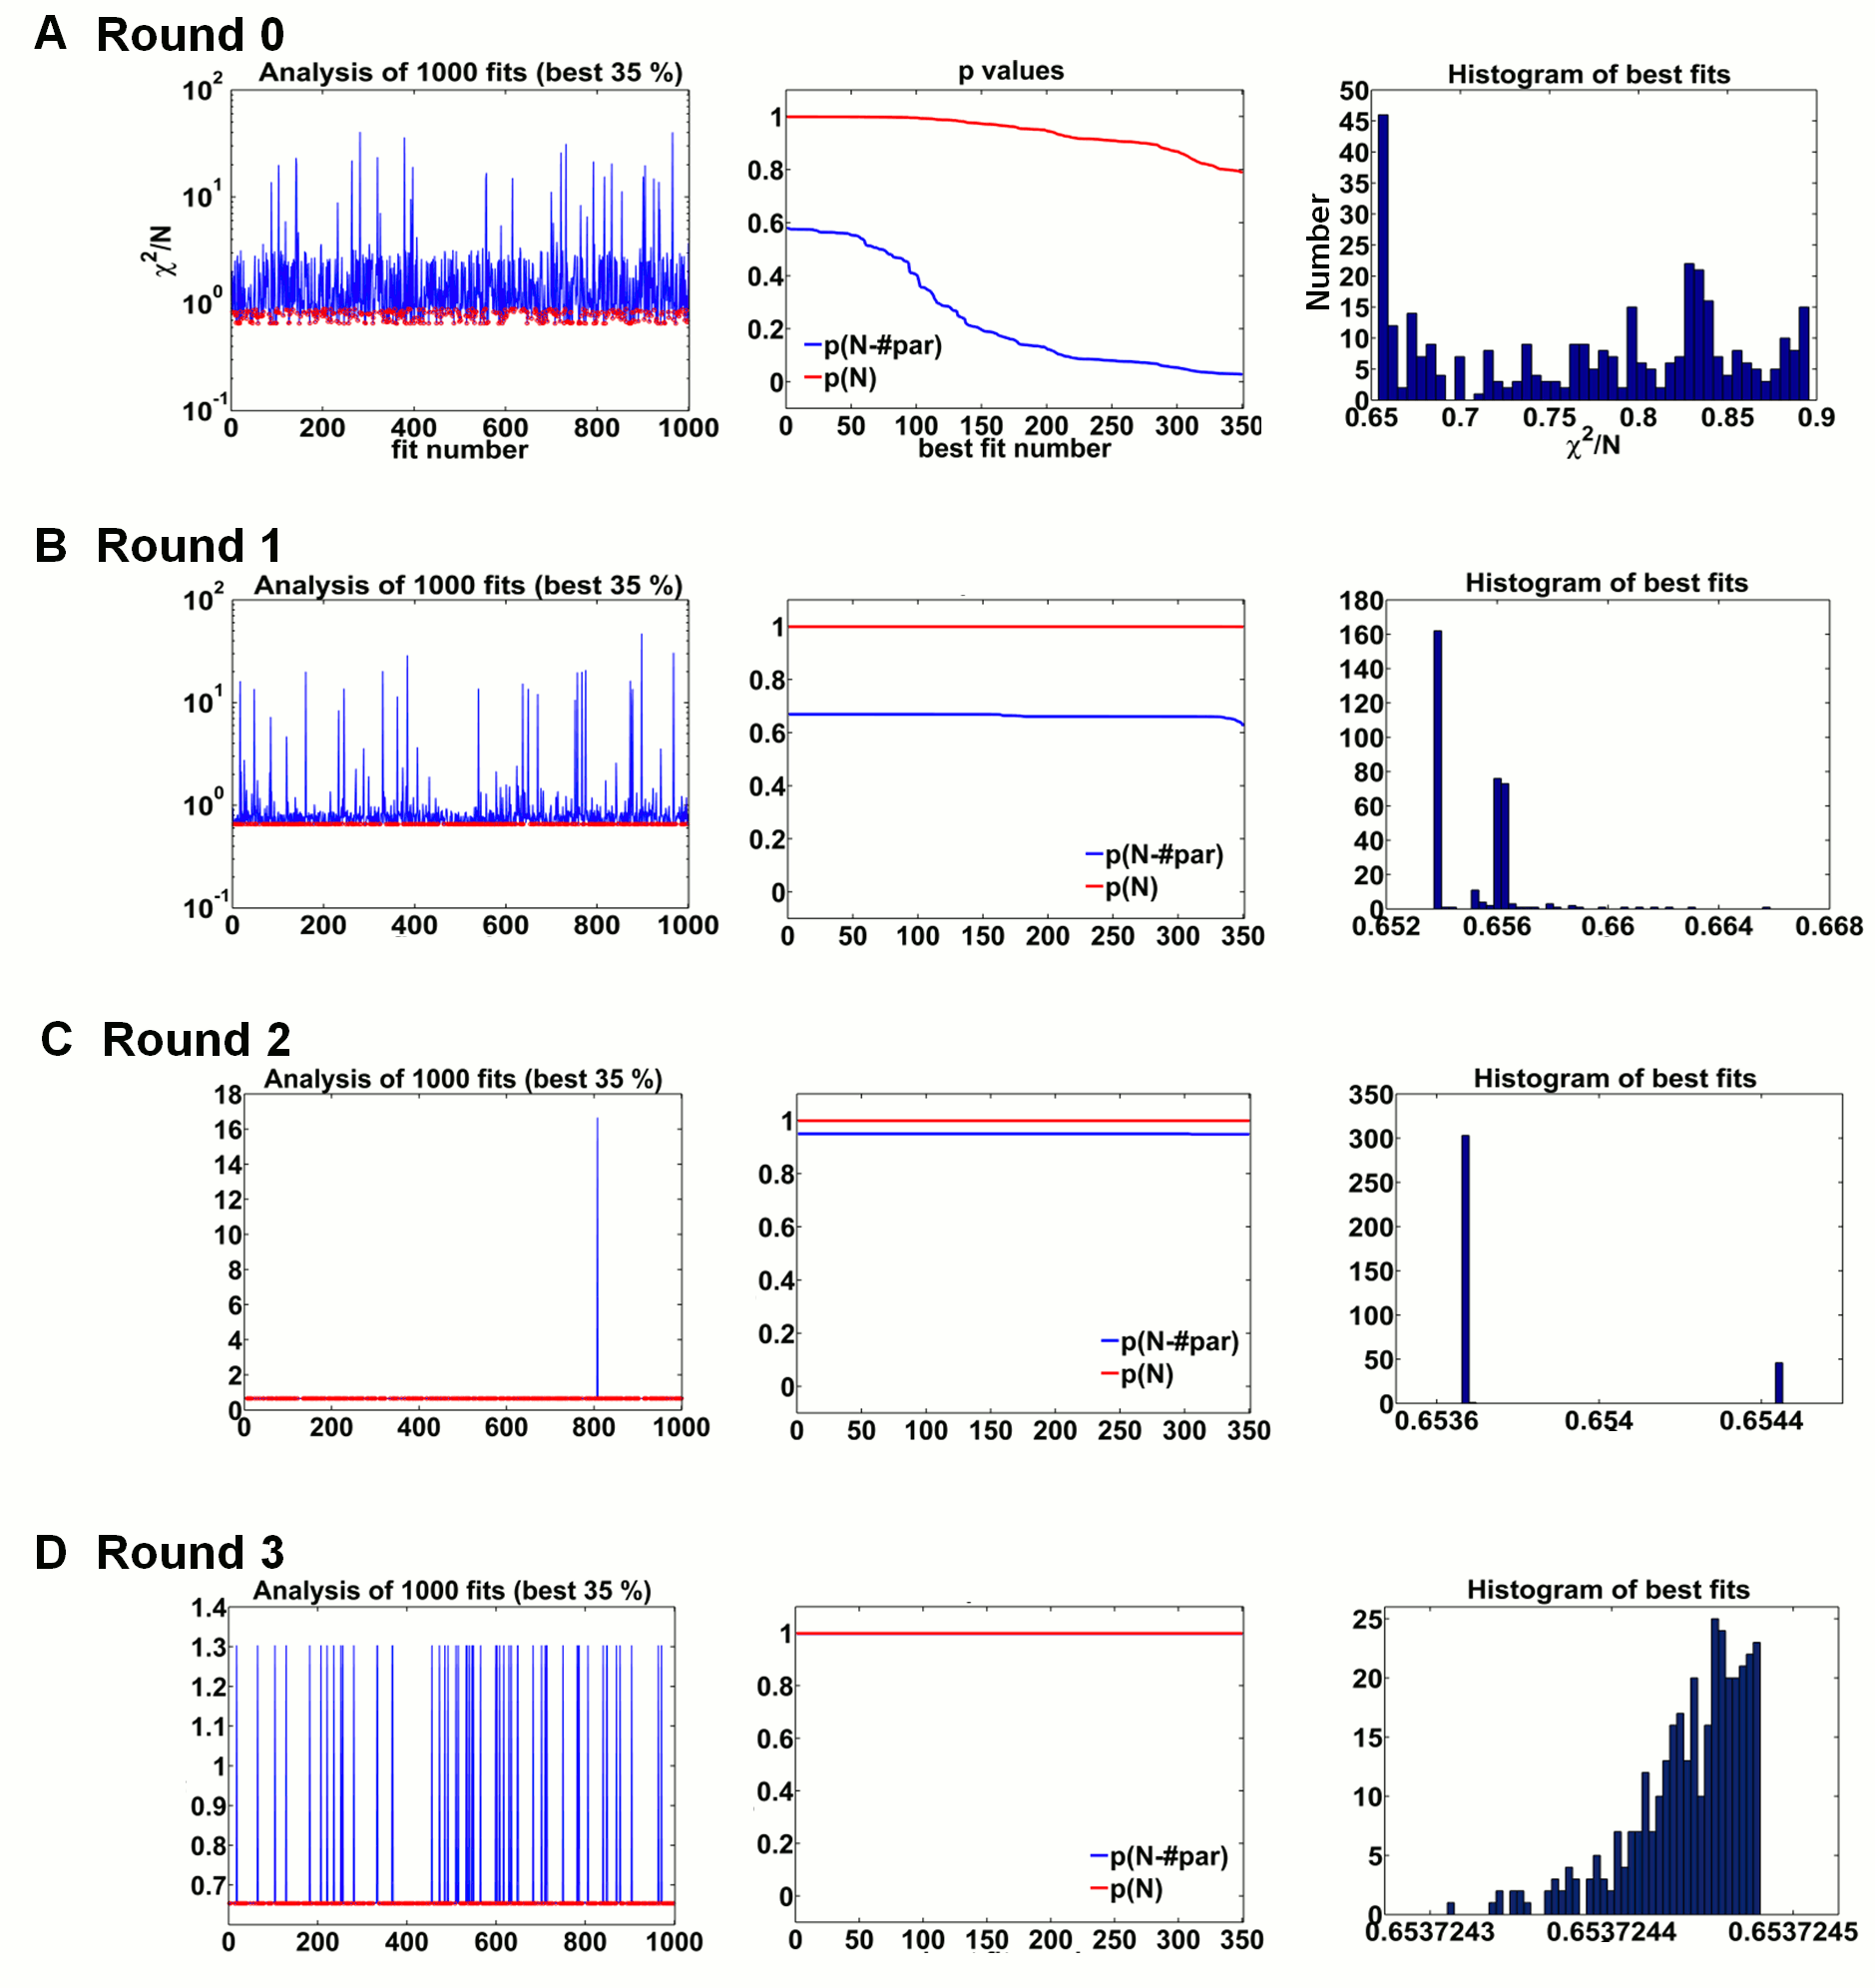
\includegraphics[scale=0.7]{linear_sequence_analysis.png}
		\caption[Sequence fits selection for parameter estimation round]{Sequence fits selection for parameter estimation round. For each calibration round, a sequence of 1000 fits was computed (see Table \ref{tab:project3_kinetic_rate_constants_table}). The best 350 fits of the sequence were selected and statistics regarding their p-values and normalised $\chi^2$ distribution were reported. Despite the high noise applied to the initial value of the parameters before estimation, the selected best fits clustered in each round in terms of$\chi^2$, particularly after Round 0. This suggested that the reported final $\chi^2$ of the model (see Table \ref{tab:project3_rounds_chisquare_table}) represented a point of convergence for many solutions. $N$=number of experimentally measured data point, $\#par$=number of estimated parameters, $p()$ = p-value function. }
		\label{fig:project3_linear_sequence_analysis}
	\end{center}
\end{figure}
\clearpage

\begin{figure}[tb]
	\begin{center}
		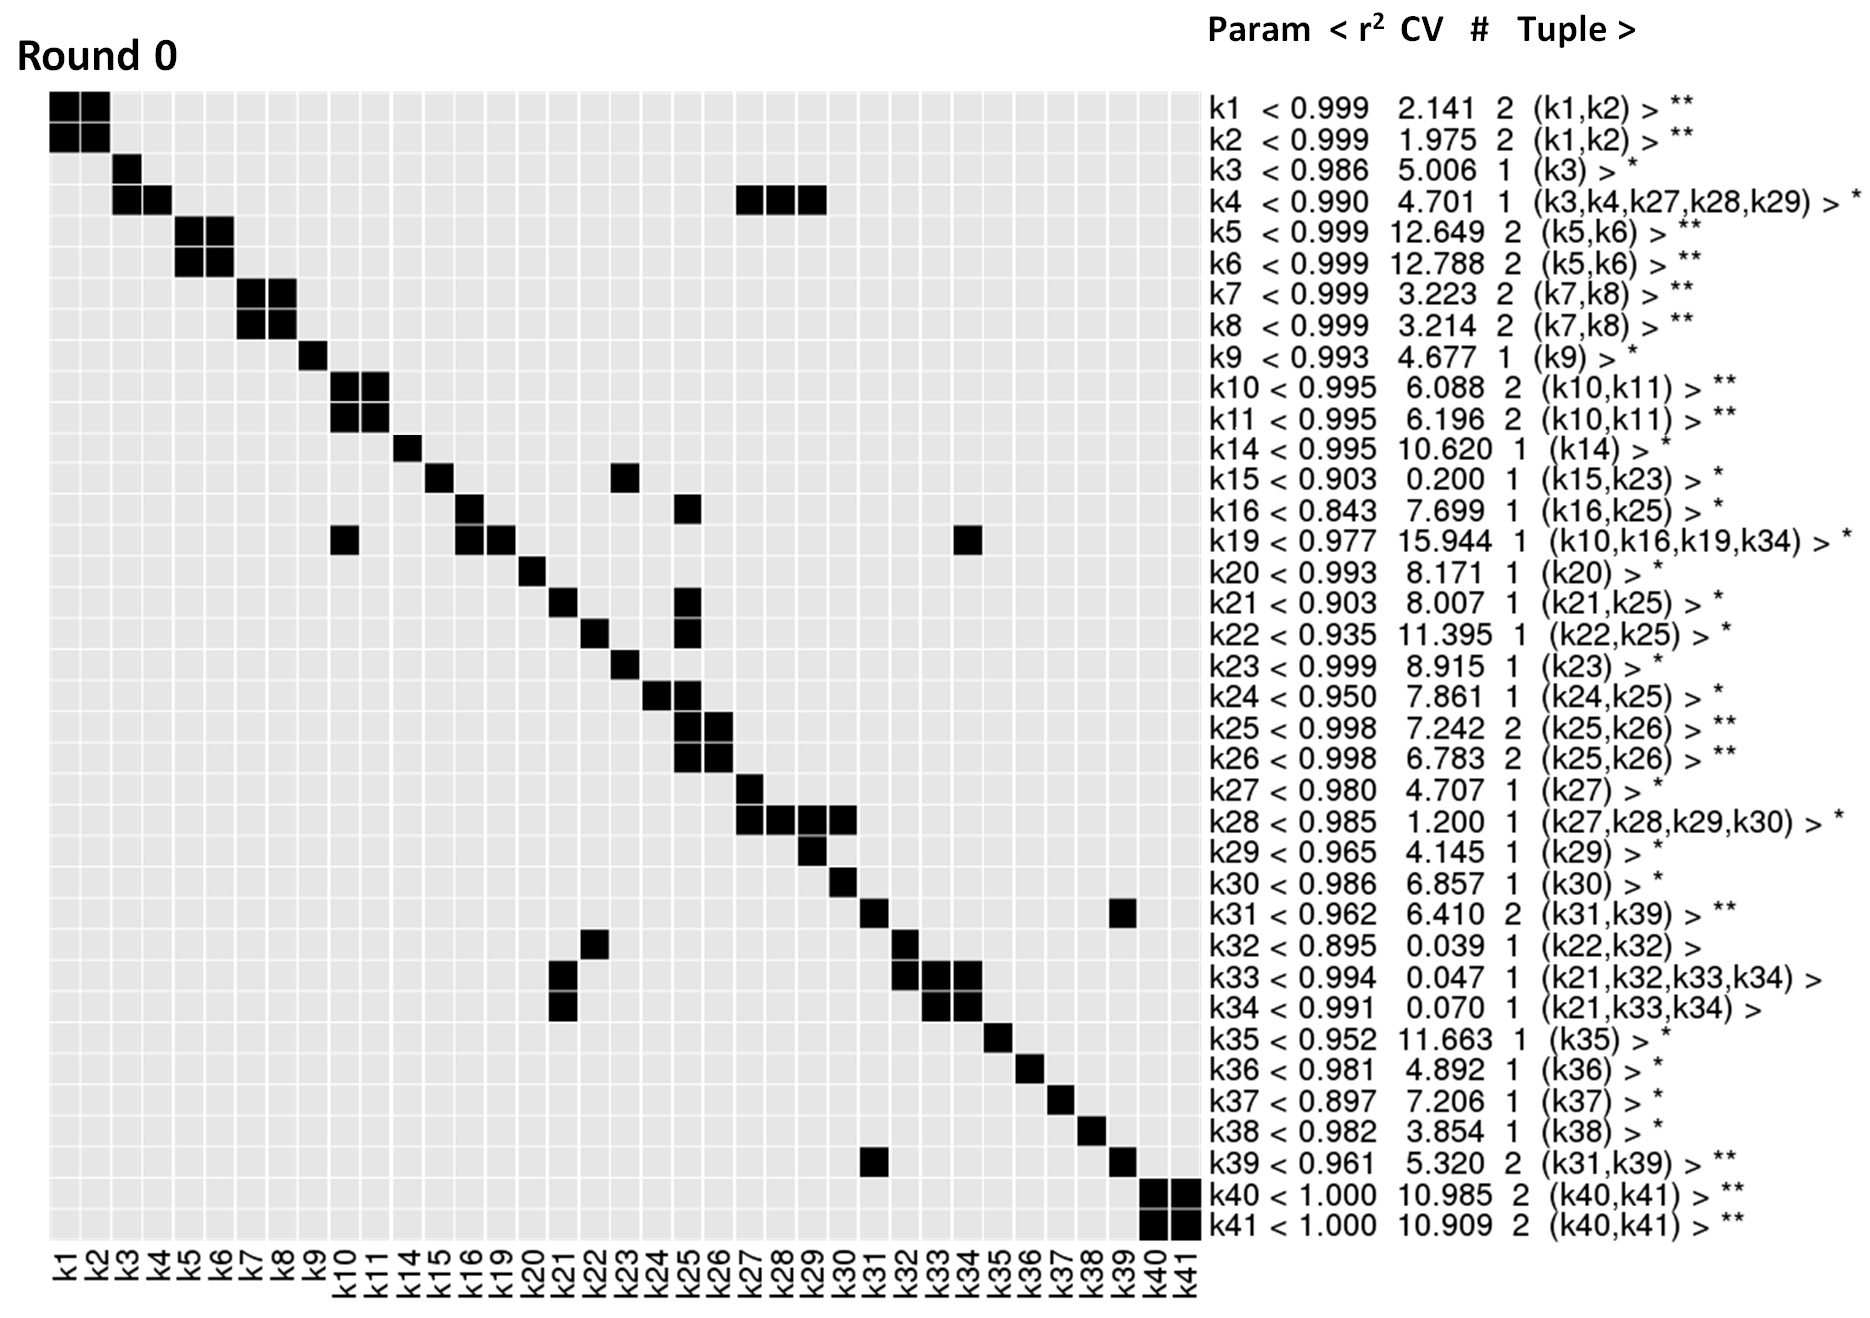
\includegraphics[scale=0.75]{round0_ident_analysis.png}
		\caption[MOTA non-identifiability analysis for Round 0 of parameter estimation]{MOTA non-identifiability analysis for Round 0 of parameter estimation. MOTA non-identifiability analysis reported multiple tuples of statistically significant parameter correlations. However, the parameters k32, k33, k34 governing the DNA-damage module could be fixed since no statistically significant correlation was found and their confidence intervals could be measured. The analysis was performed on the best 35\% fits of the calibration sequence without excluding any outlier. $r^2$=correlation, CV=coefficient of variance, \#=number of times this correlation was found. (*) $r^2 > 0.8$ \& $CV > 0.1$  (**) $r^2 > 0.8$ \& $CV > 0.1$ \& \#$> 1$.}
		\label{fig:project3_round0_ident_analysis}
	\end{center}
\end{figure}
\clearpage

\begin{figure}[tb]
	\begin{center}
		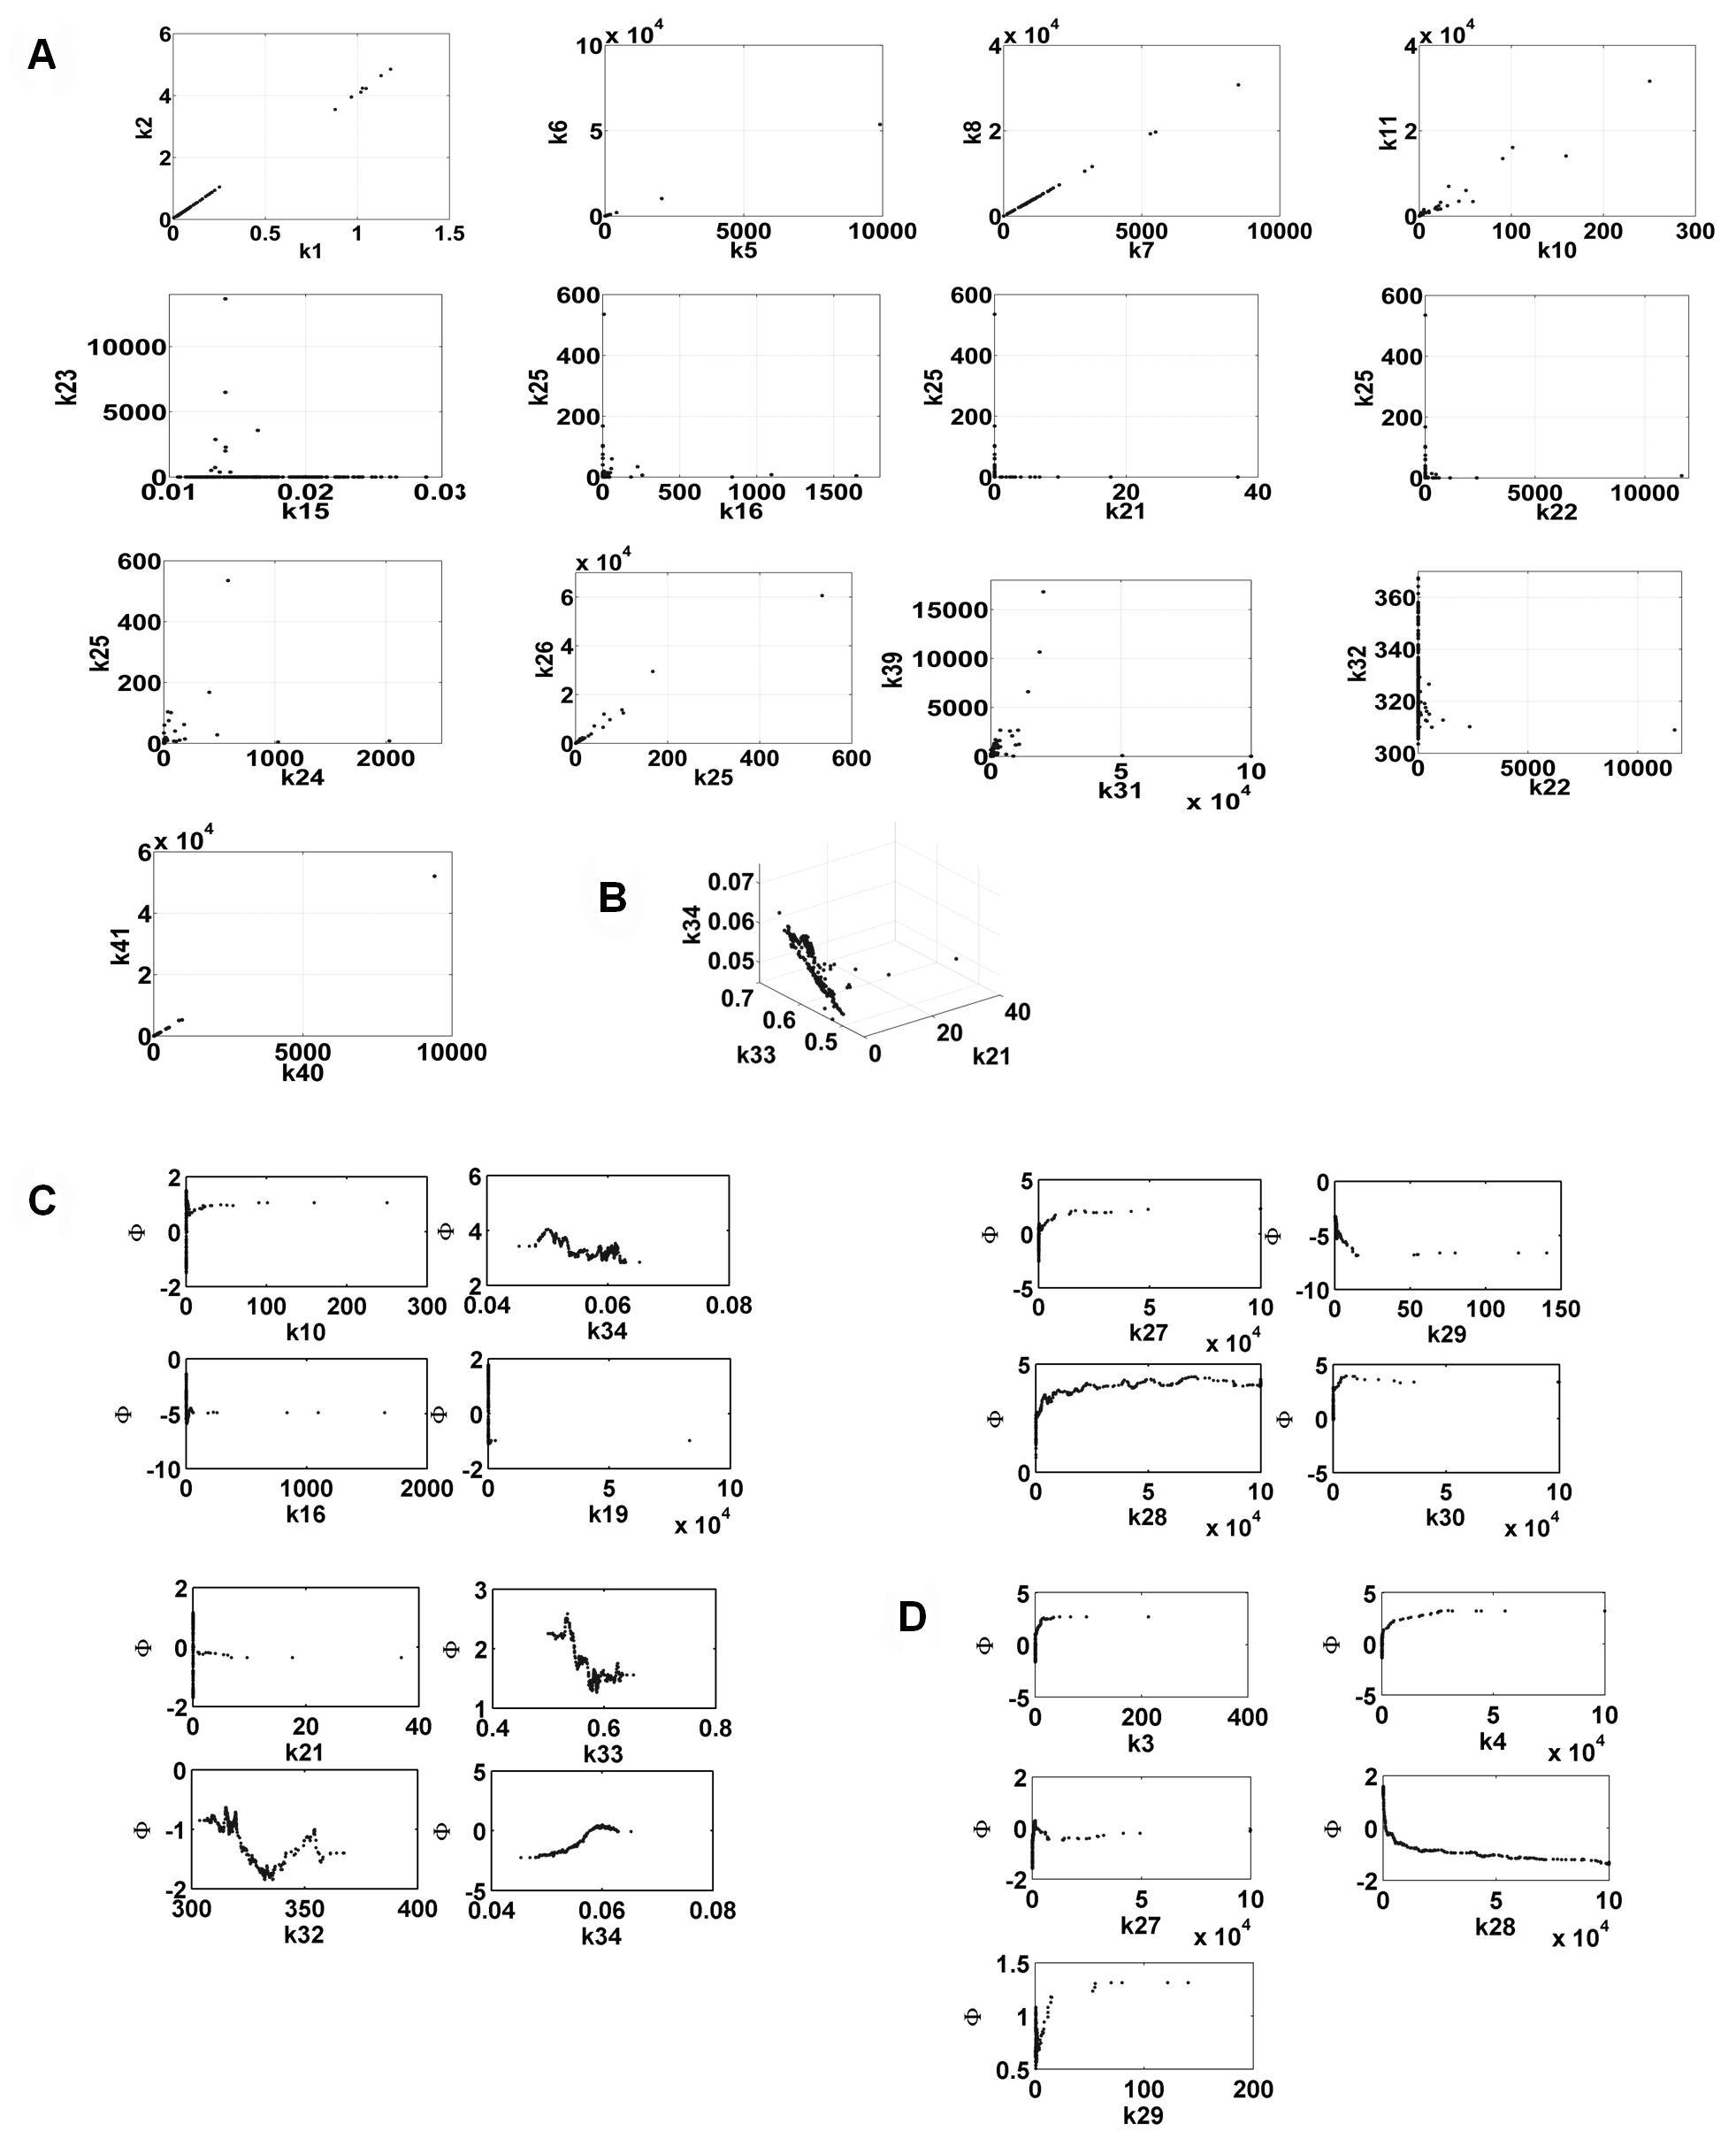
\includegraphics[scale=0.75]{round0_ident_analysis_plots.png}
		\caption[Plots of tuples of related parameters for Round 0]{Plots of tuples of related parameters for Round 0. Doublets (A), triplets (B), quadruplets (C) and quintuplets (D) of related parameters as computed by MOTA non-identifiability analysis (see Figure \ref{fig:project3_round0_ident_analysis}) are shown. The analysis was performed over the best 35\% of the fit sequence.}
		\label{fig:project3_round0_ident_analysis_plots}
	\end{center}
\end{figure}
\clearpage

\begin{figure}[tb]
	\begin{center}
		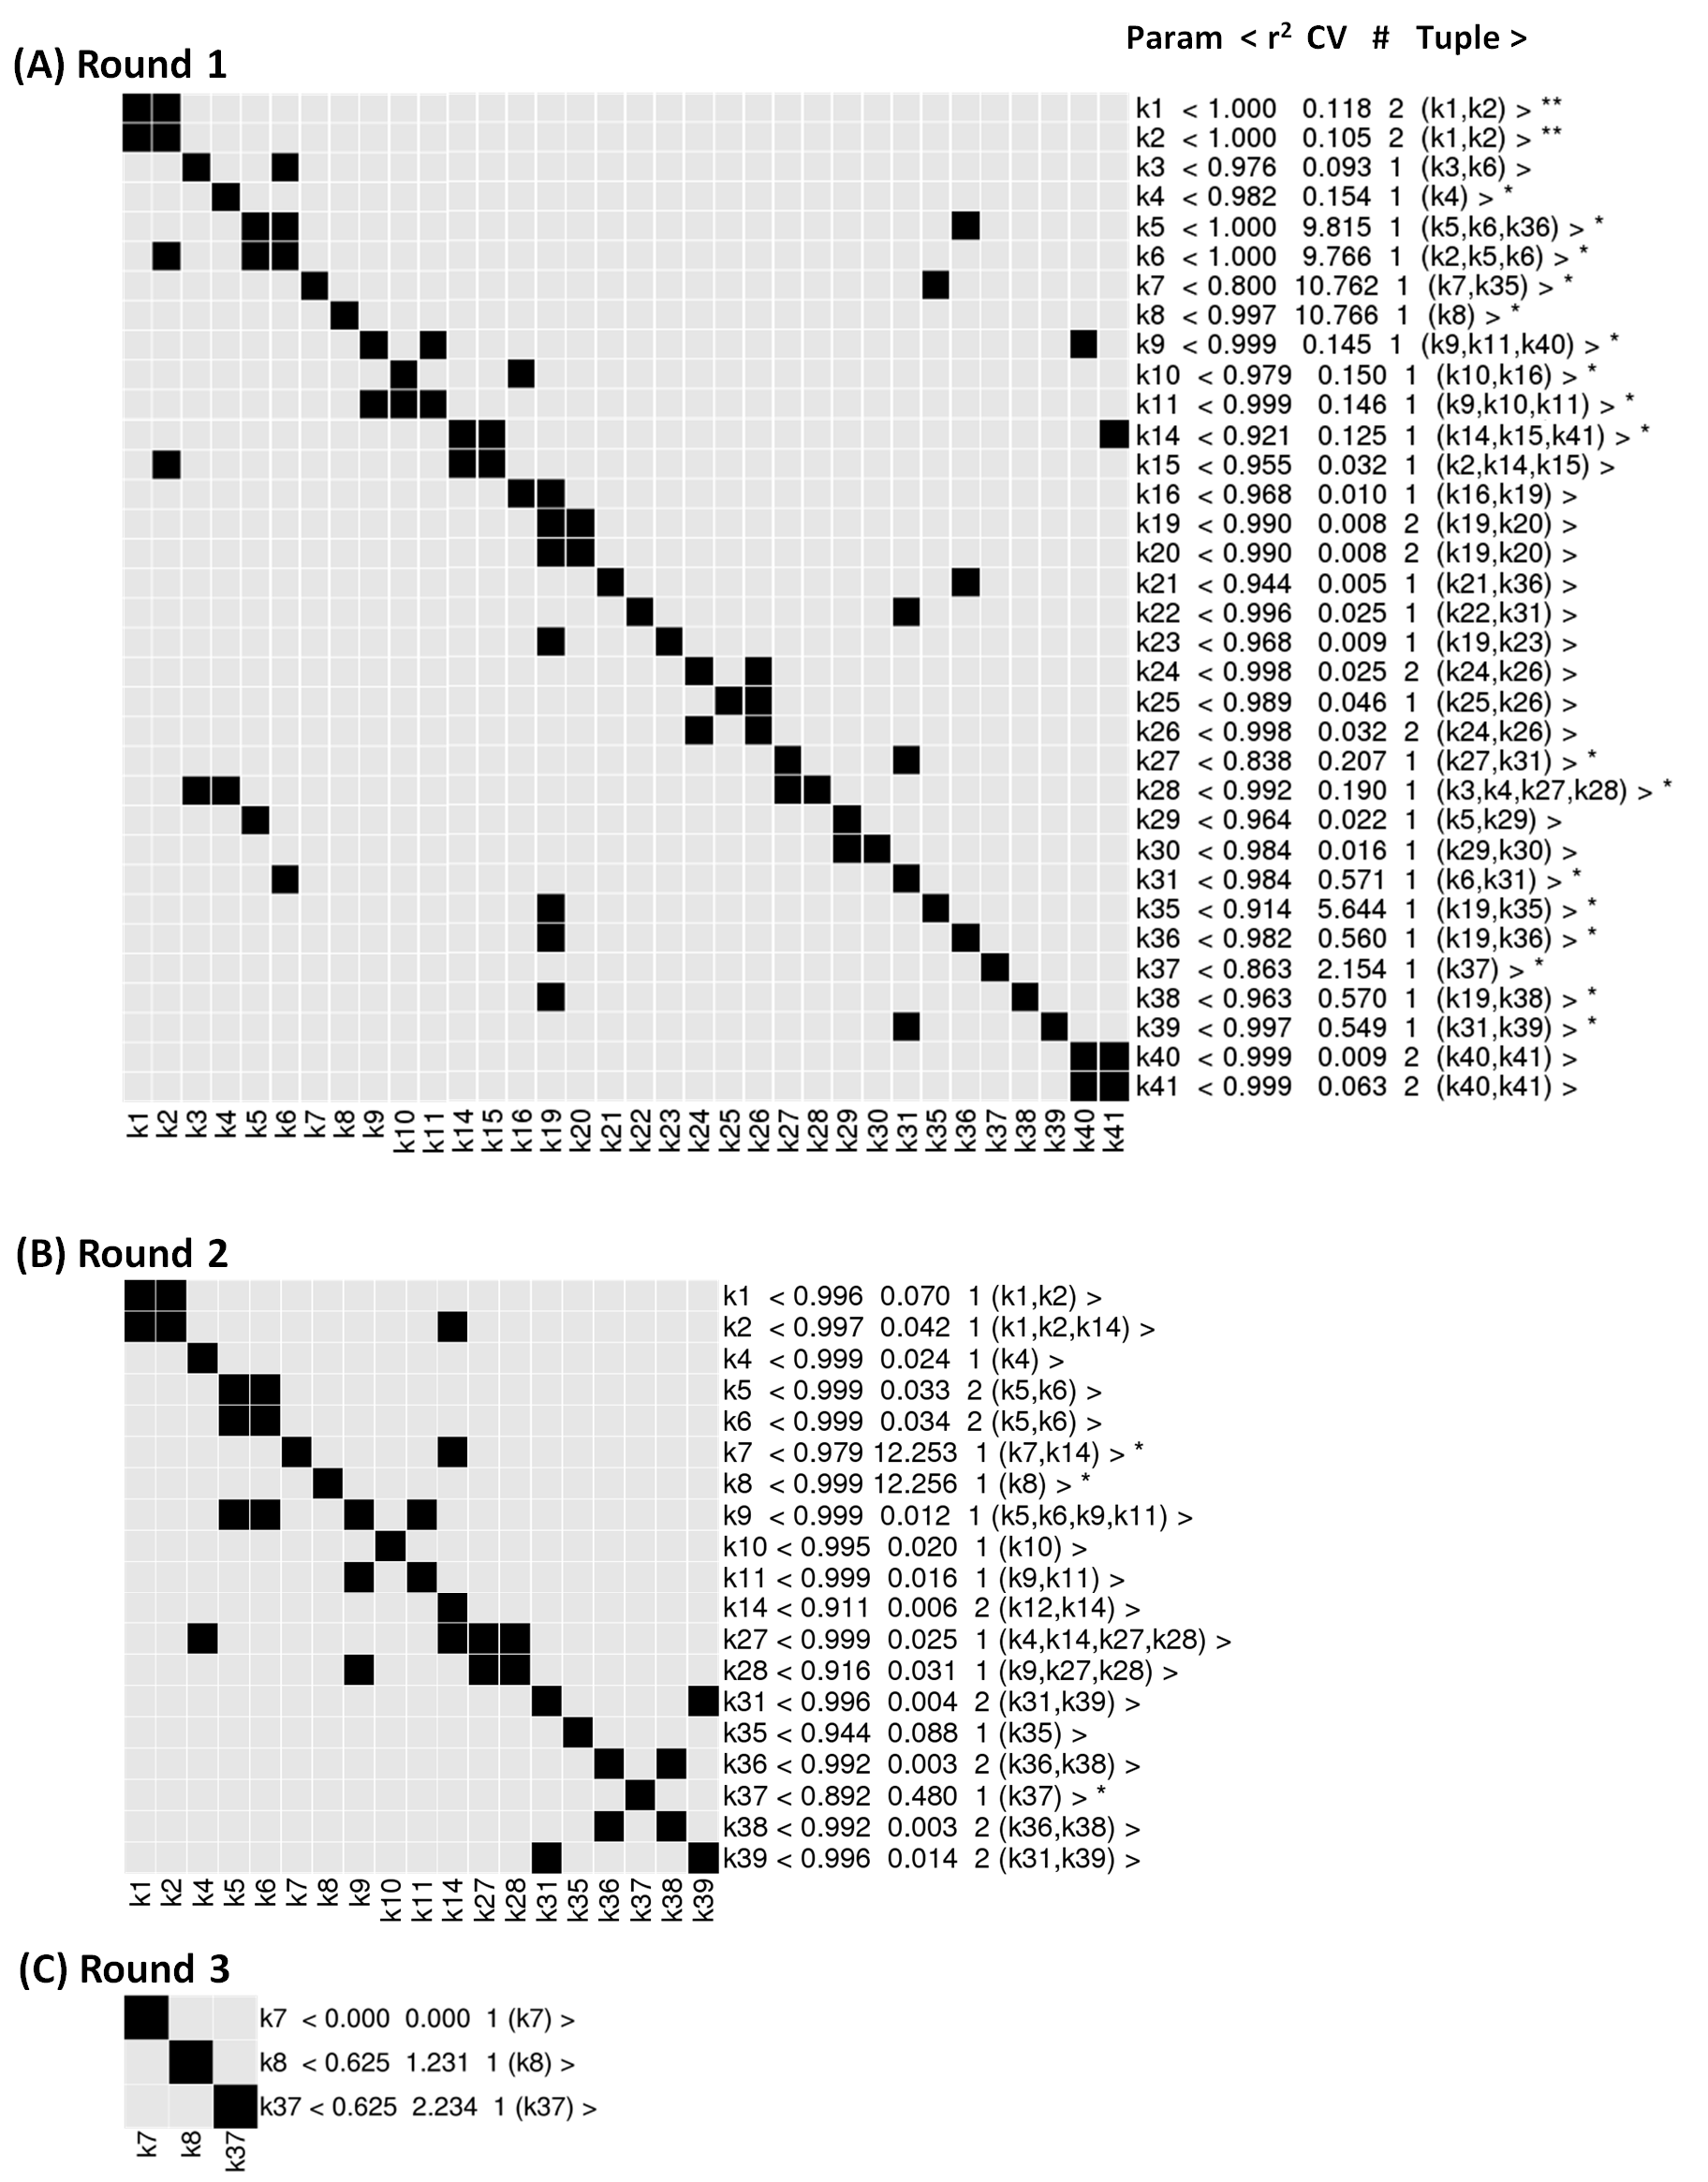
\includegraphics[scale=0.75]{round123_ident_analysis.png}
		\caption[MOTA non-identifiability analysis for Round 1,2 and 3 of parameter estimation]{MOTA non-identifiability analysis for Round 1,2 and 3 of parameter estimation. (A) In Round 1, most of the parameters did not show statistically significant correlations and could therefore be fixed. (B) Round 2 only reported 3 parameters as non-identifiable which were finally determined in Round 3 (C). For each round, the analysis was performed on the best 35\% fits of the calibration sequence without excluding any outlier. $r^2$=correlation, CV=coefficient of variance, \#=number of times this correlation was found. (*) $r^2 > 0.8$ \& $CV > 0.1$  (**) $r^2 > 0.8$ \& $CV > 0.1$ \& \#$> 1$.}
		\label{fig:project3_round123_ident_analysis}
	\end{center}
\end{figure}
\clearpage

\begin{figure}[tb]
	\begin{center}
		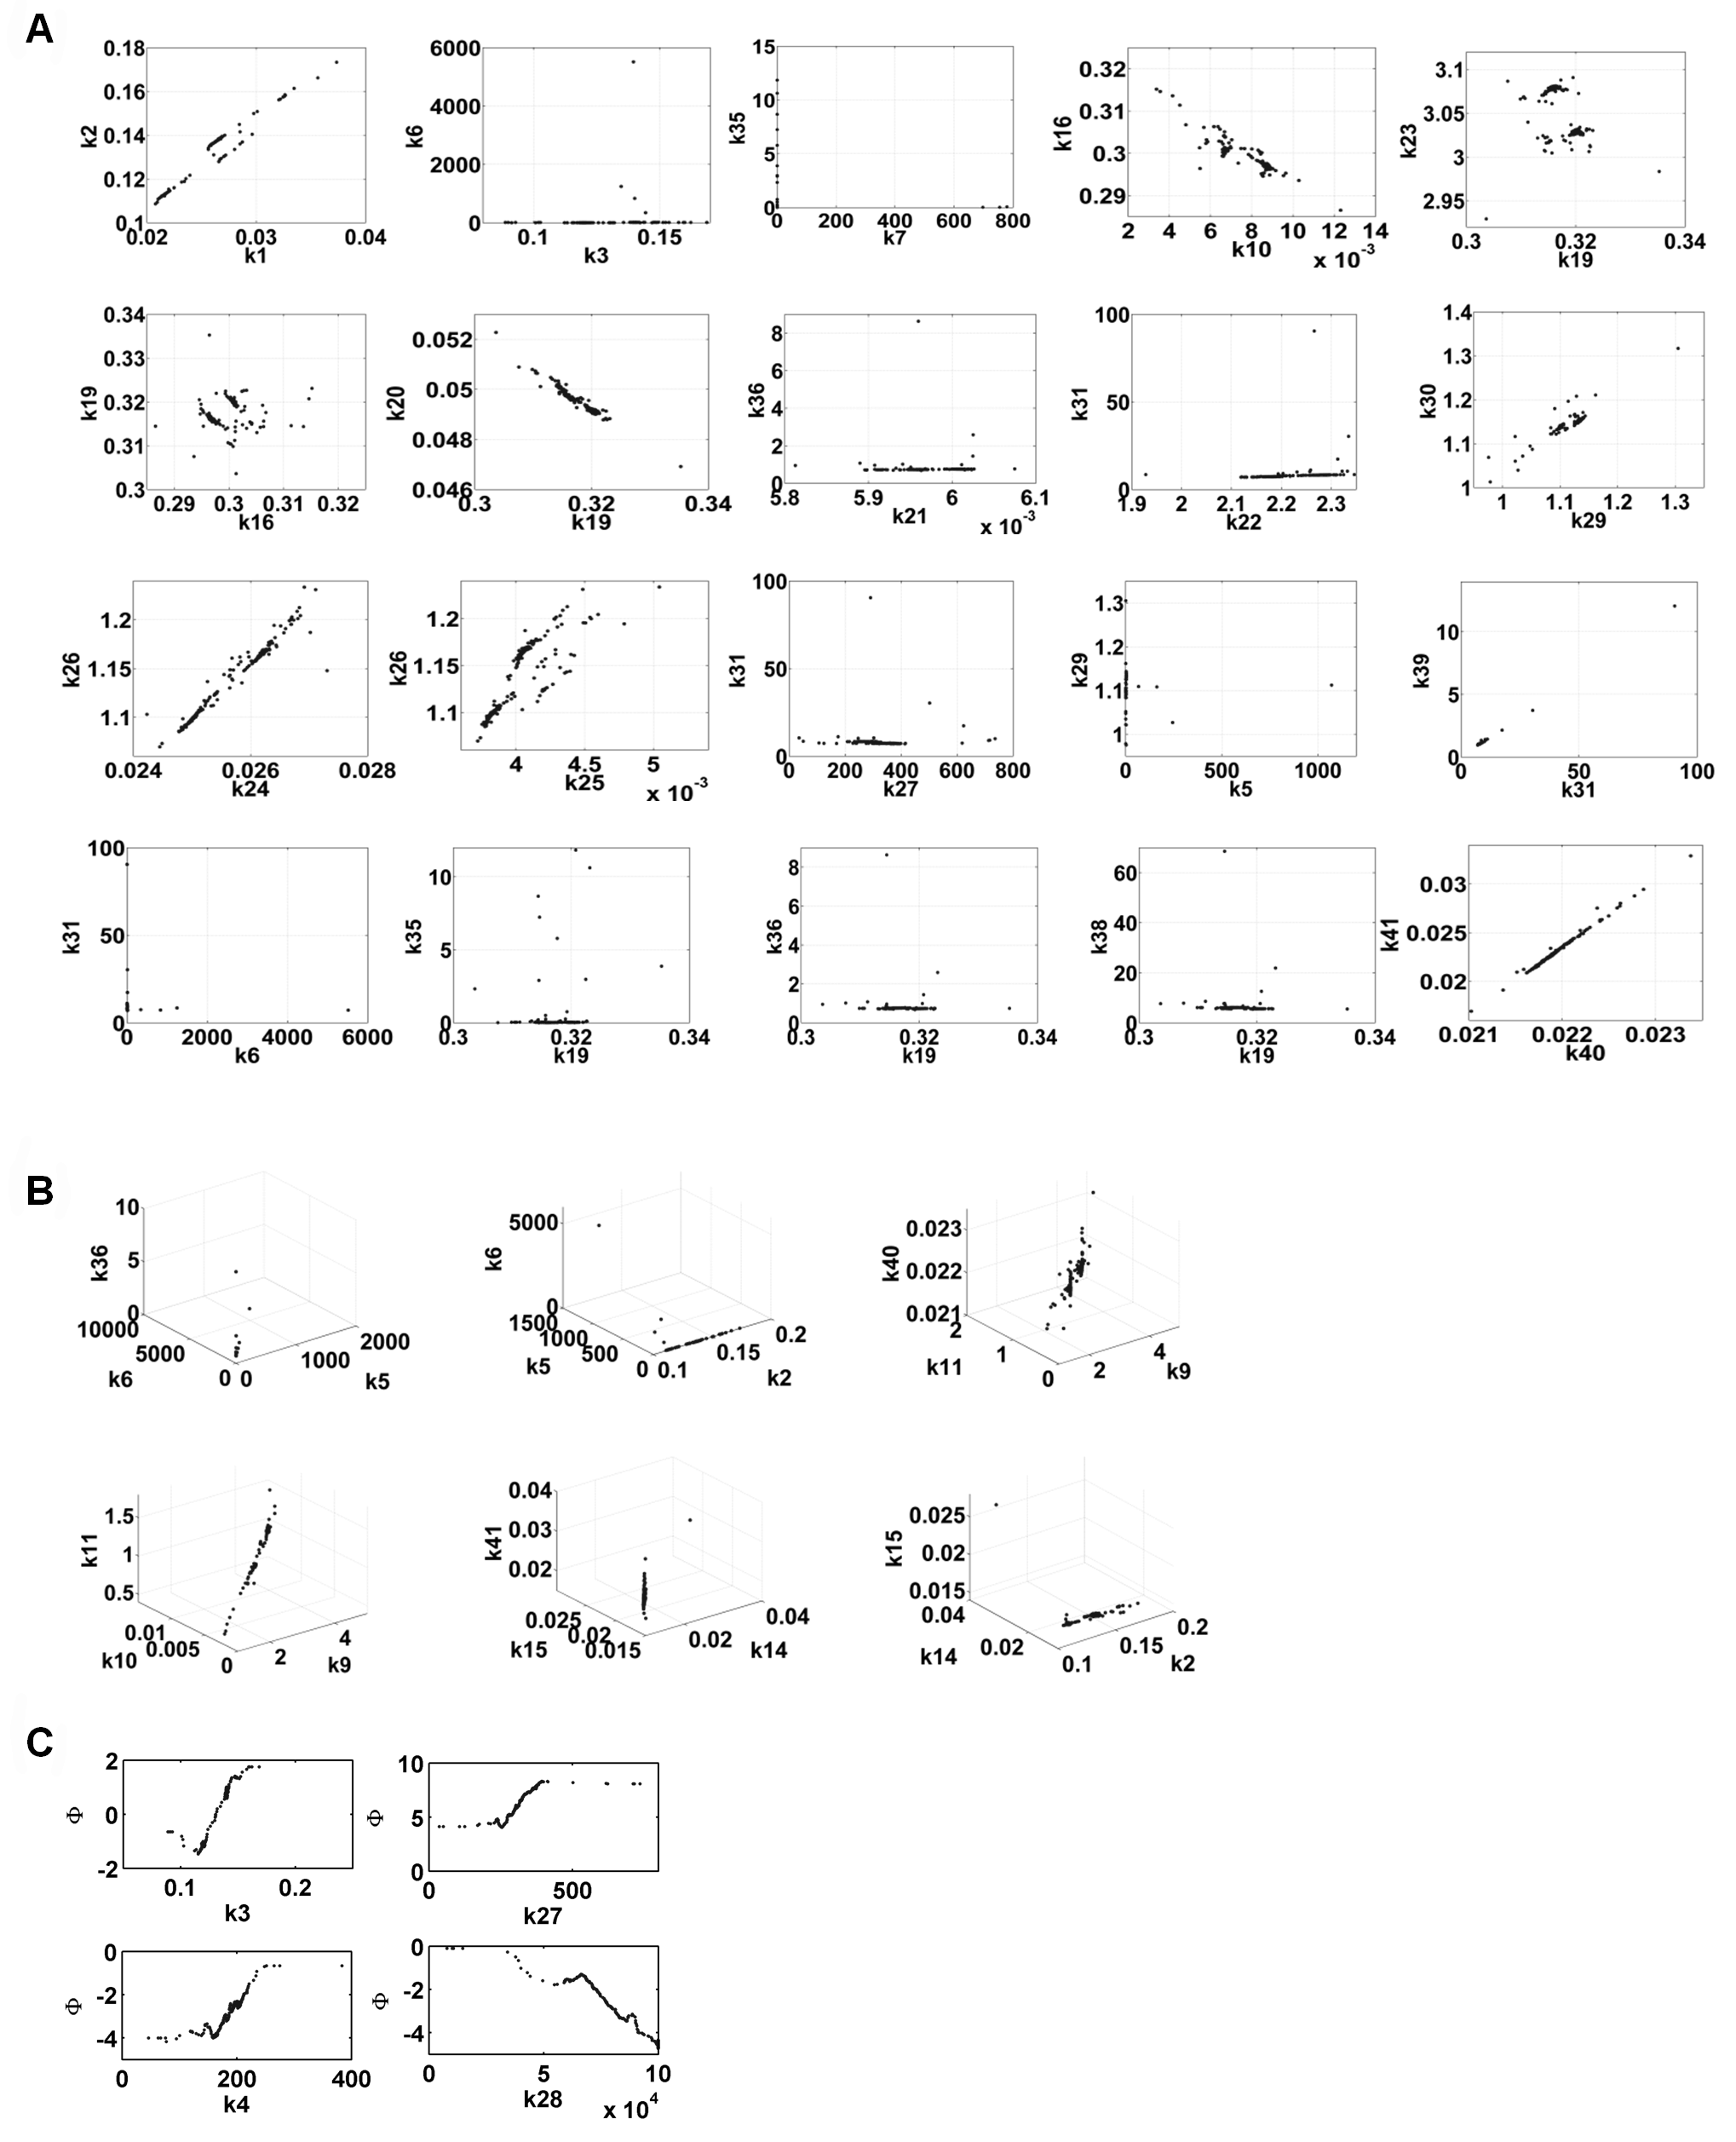
\includegraphics[scale=0.75]{round1_ident_analysis_plots.png}
		\caption[Plots of tuples of related parameters for Round 1]{Plots of tuples of related parameters for Round 1. Doublets (A), triplets (B) and quadruplets (C) of related parameters as computed by MOTA non-identifiability analysis (see Figure \ref{fig:project3_round123_ident_analysis}) are shown. The analysis was performed over the best 35\% of the fit sequence.}
		\label{fig:project3_round1_ident_analysis_plots}
	\end{center}
\end{figure}
\clearpage

\begin{figure}[tb]
	\begin{center}
		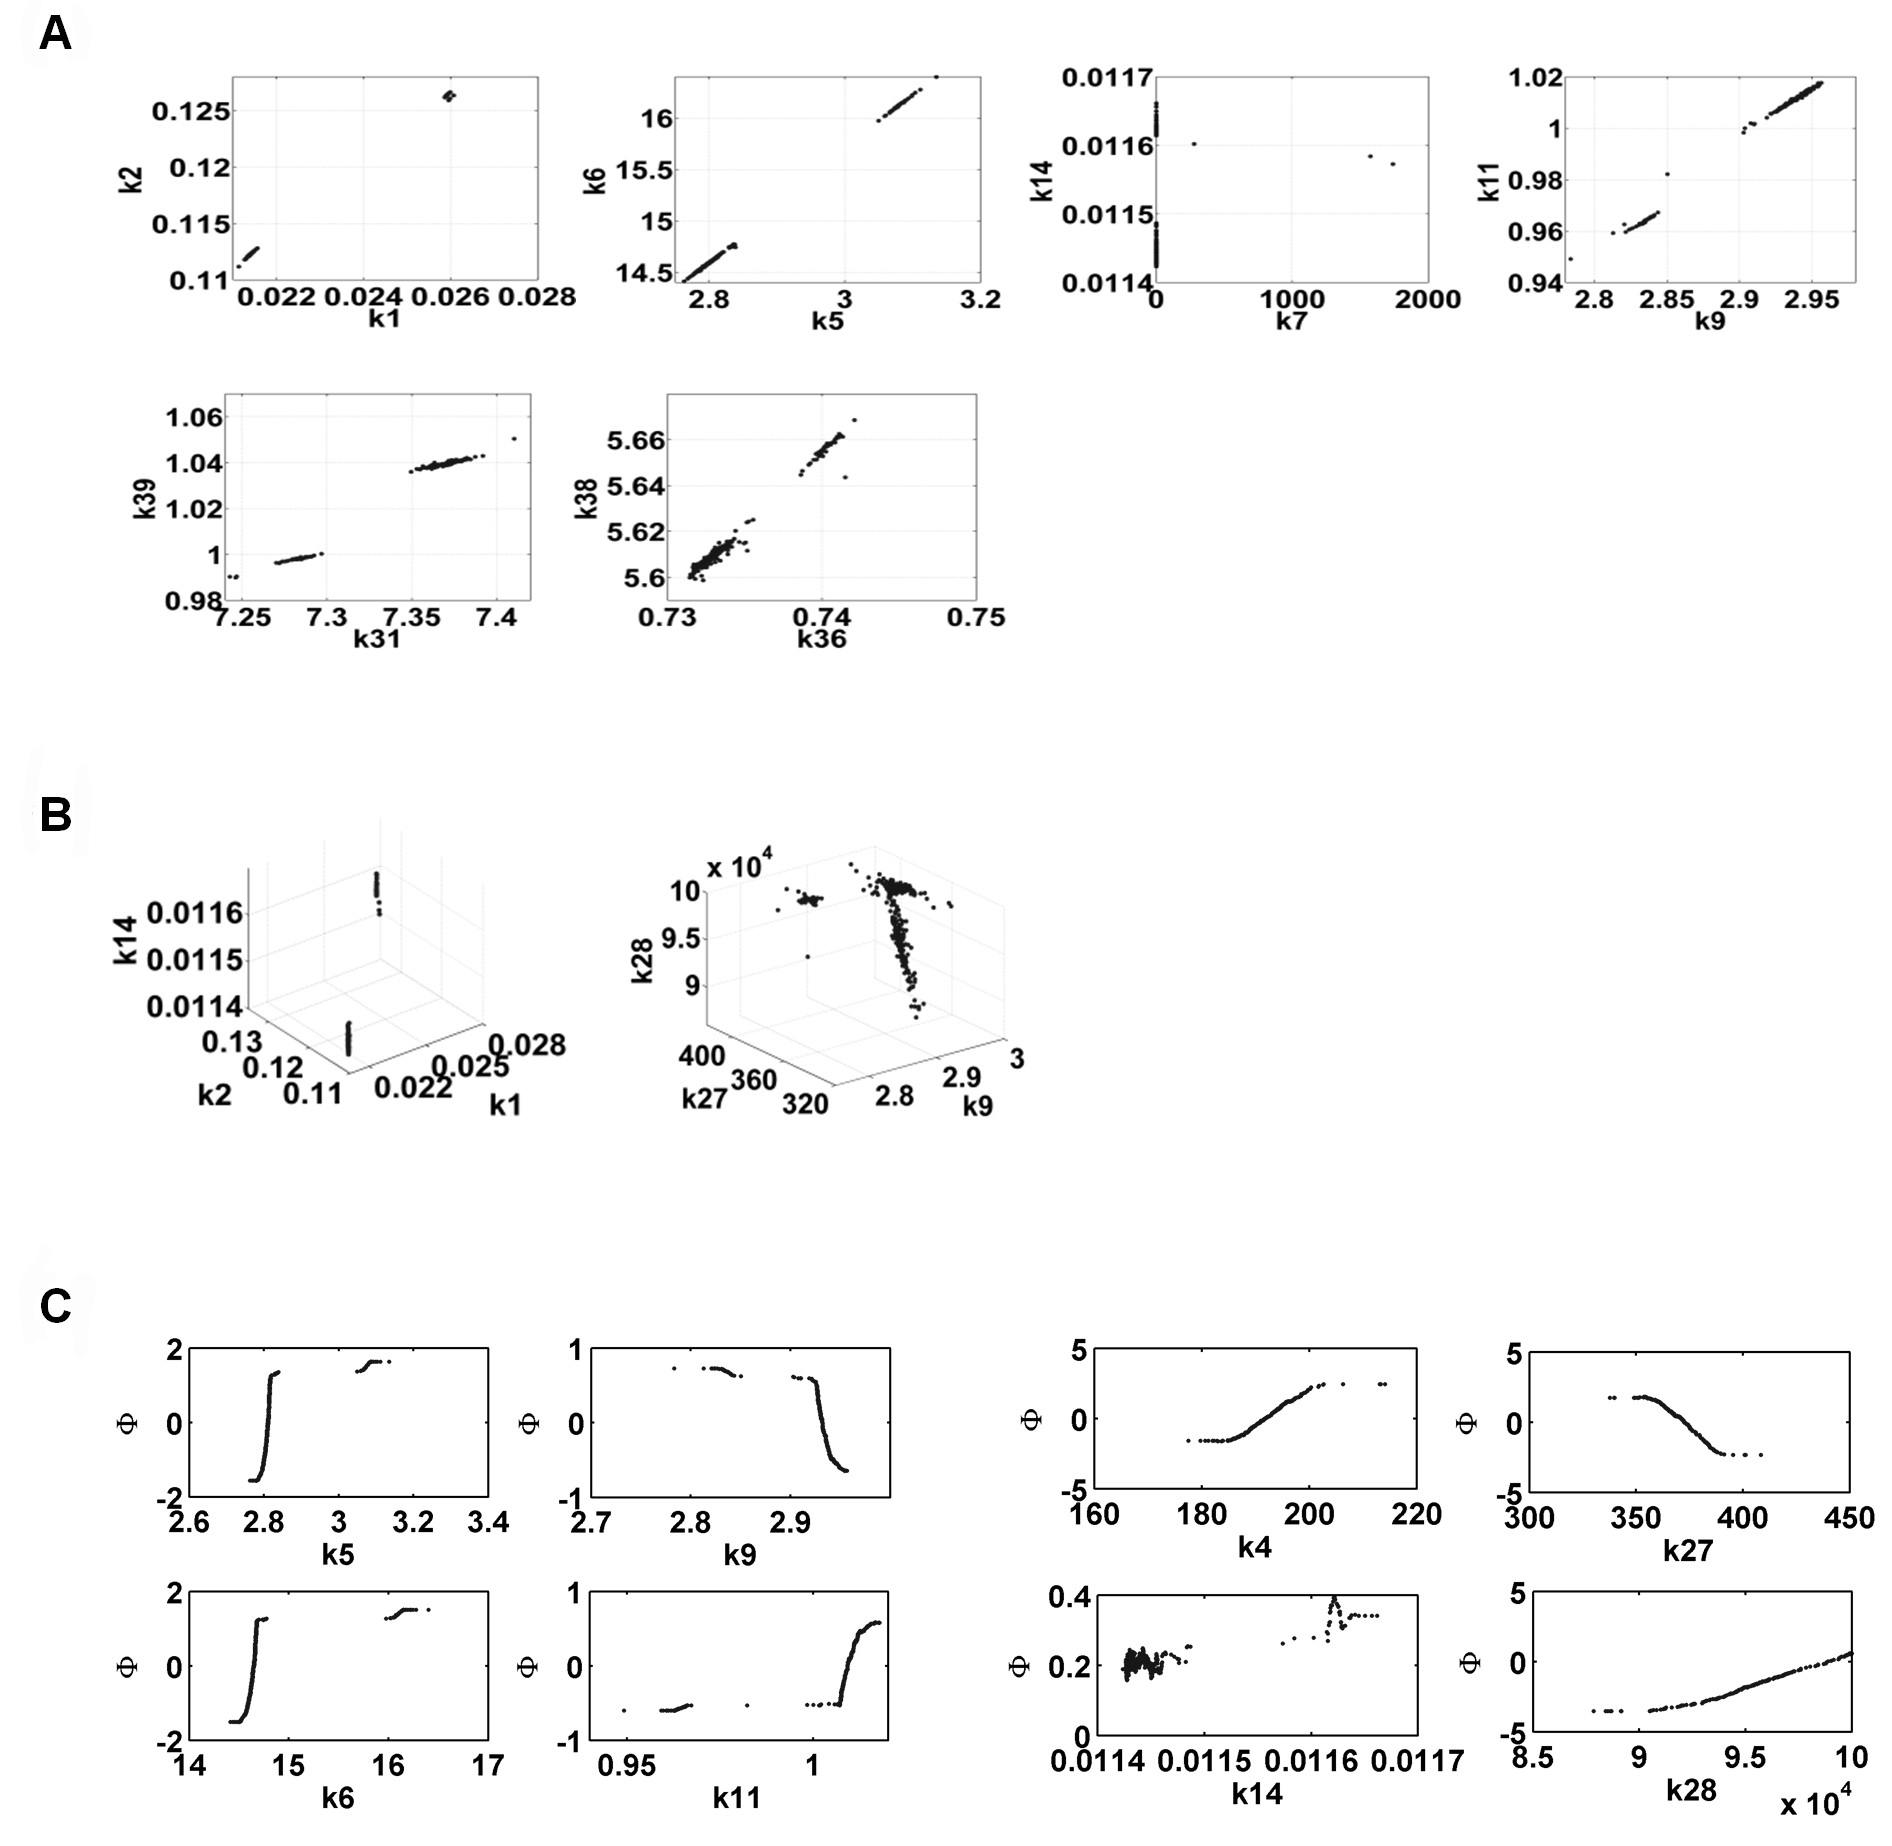
\includegraphics[scale=0.75]{round2_ident_analysis_plots.png}
		\caption[Plots of tuples of related parameters for Round 2]{Plots of tuples of related parameters for Round 2. Doublets (A), triplets (B) and quadruplets (C) of related parameters as computed by MOTA non-identifiability analysis (see Figure \ref{fig:project3_round123_ident_analysis}) are shown. The analysis was performed over the best 35\% of the fit sequence.}
		\label{fig:project3_round2_ident_analysis_plots}
	\end{center}
\end{figure}
\clearpage

\begin{figure}[tb]
	\begin{center}
		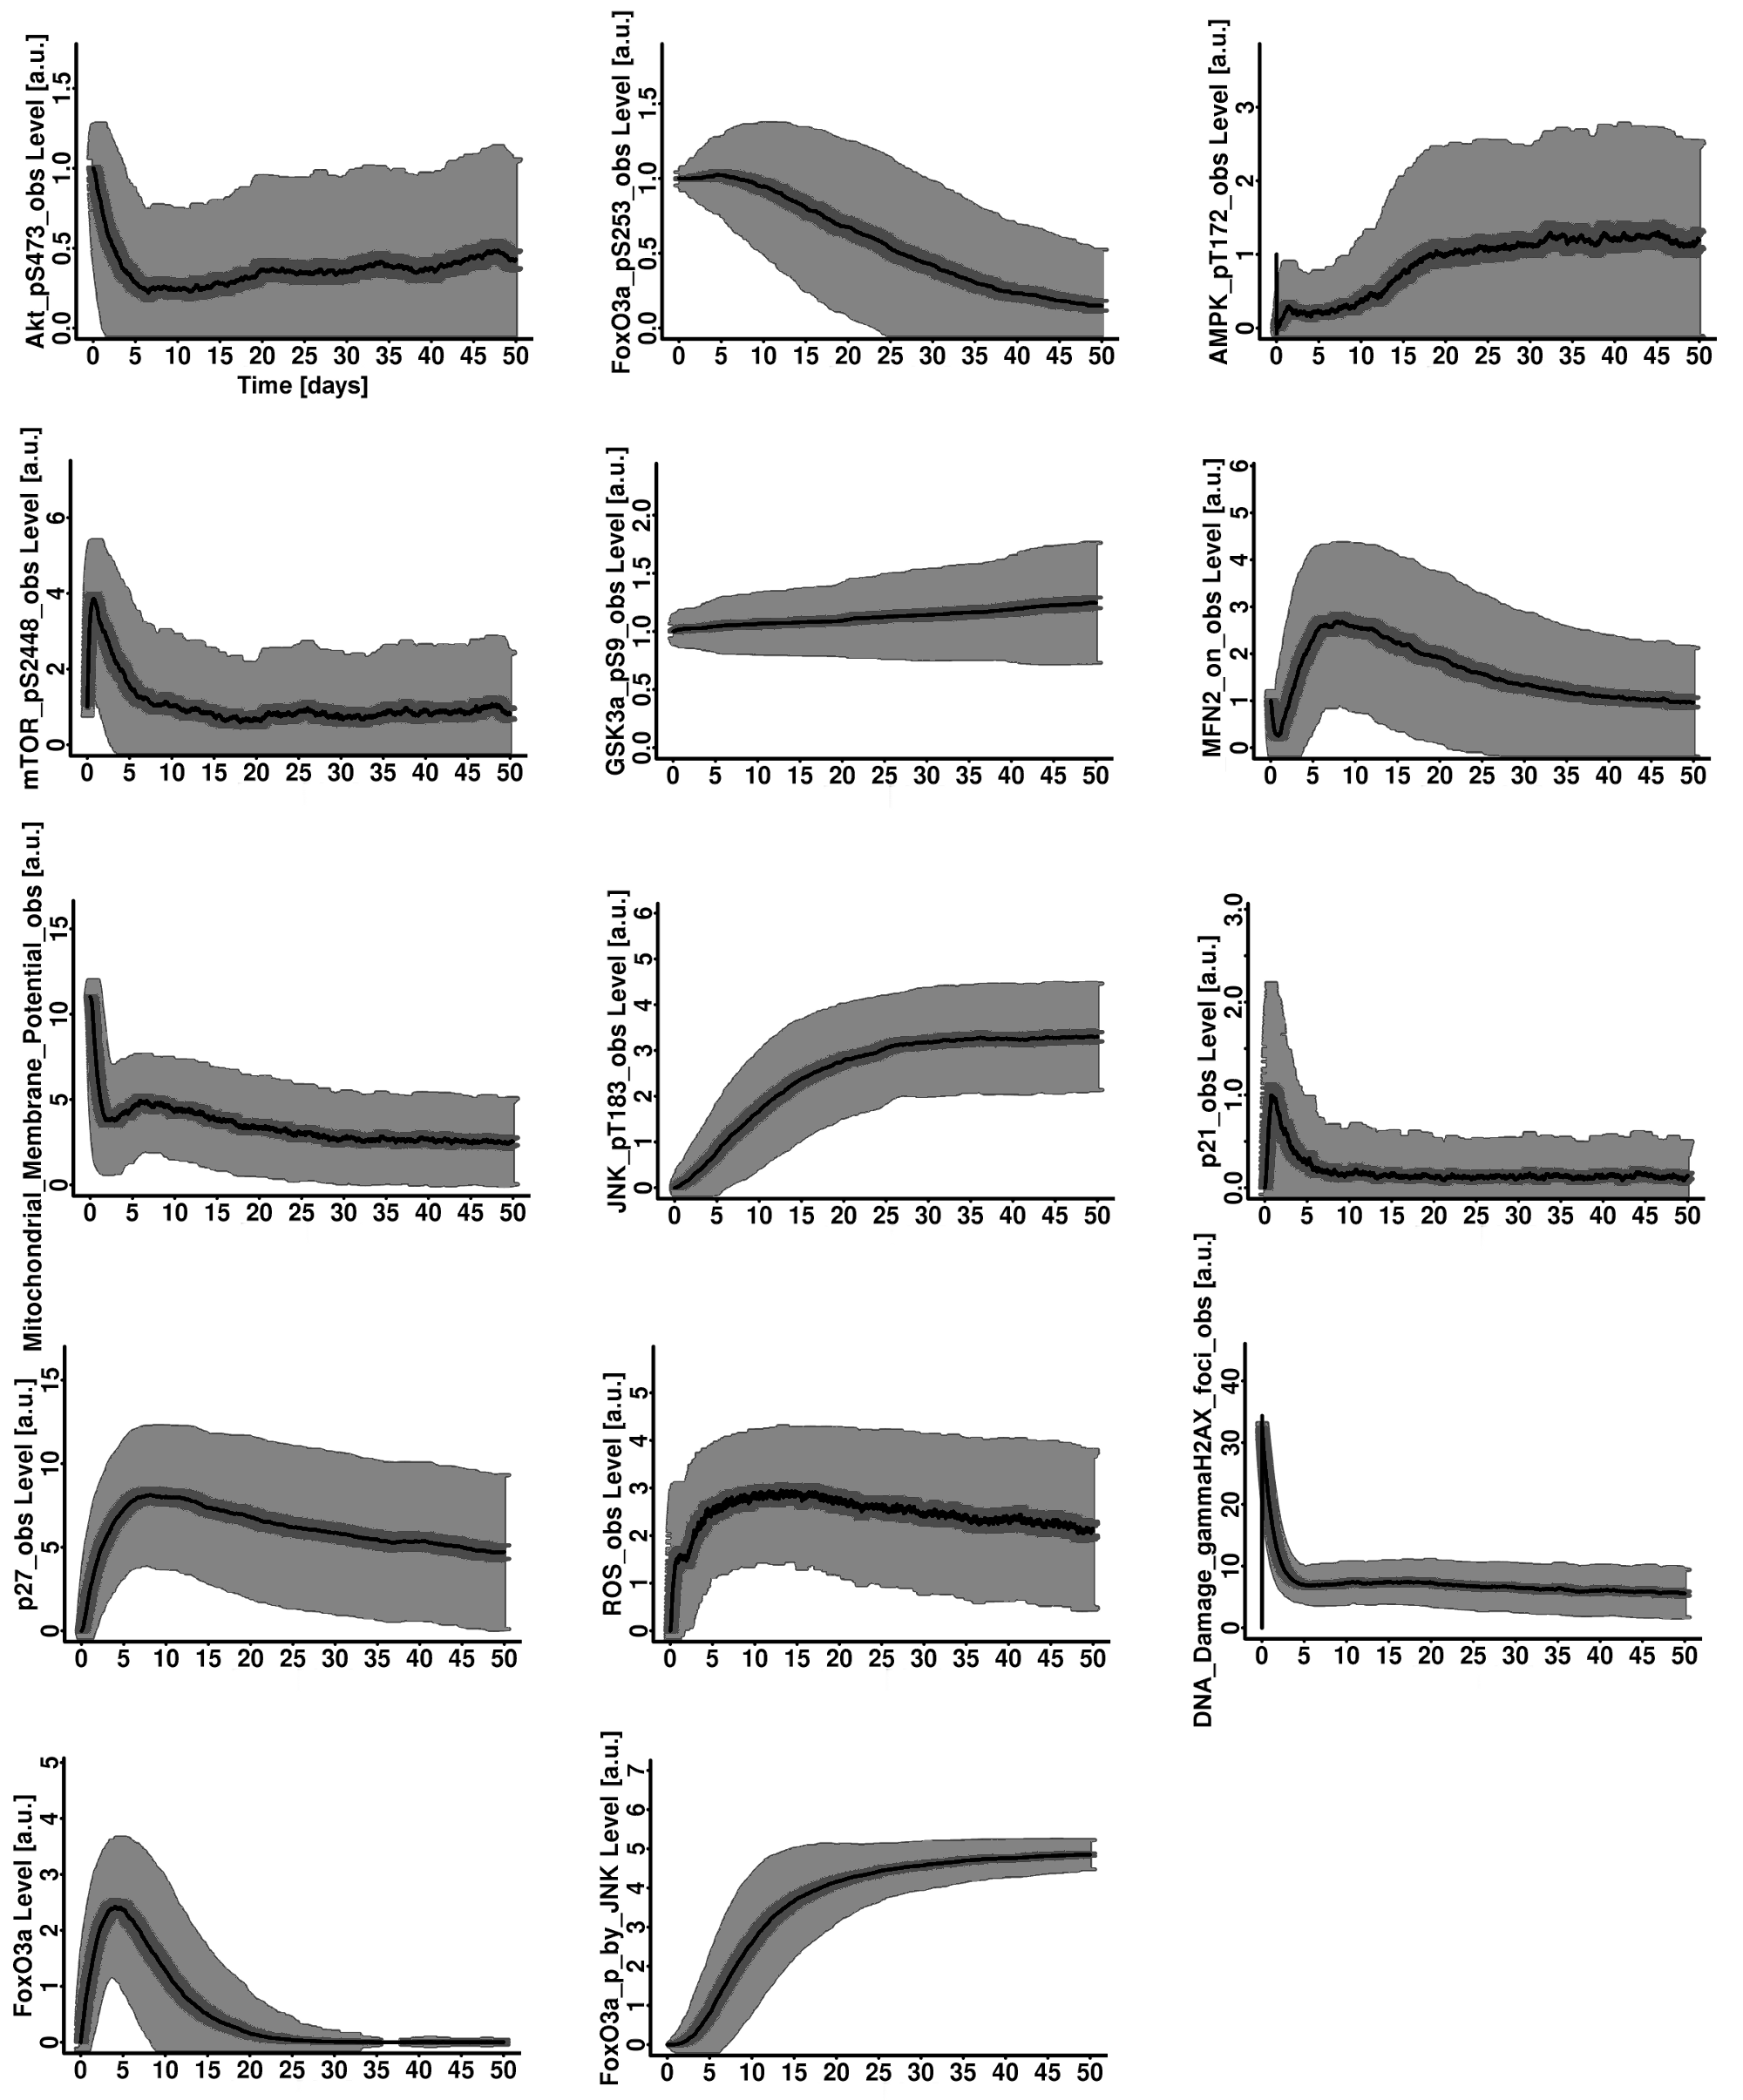
\includegraphics[scale=0.7]{stochastic_simulations.png}
		\caption[Stochastic simulation of the model]{Stochastic simulation of the model. Model stochastic simulations up to 50 days graphically showed steady-state already after 20 days for all the species. Due to high ROS levels, the oxidative stress response forces almost all nuclear FoxO3a to be phosphorylated by JNK. For a formal analysis indicating that the system is asymptotically Lyapunov stable see Table \ref{tab:project3_lyapunov_exp}. Number of stochastic runs: 500; black line indicates the means, dark grey area indicates 95\% confidence interval of the mean and grey area indicates a standard deviation.}
		\label{fig:project3_stochastic_simulations}
	\end{center}
\end{figure}
\clearpage

\begin{figure}[tb]
	\begin{center}
		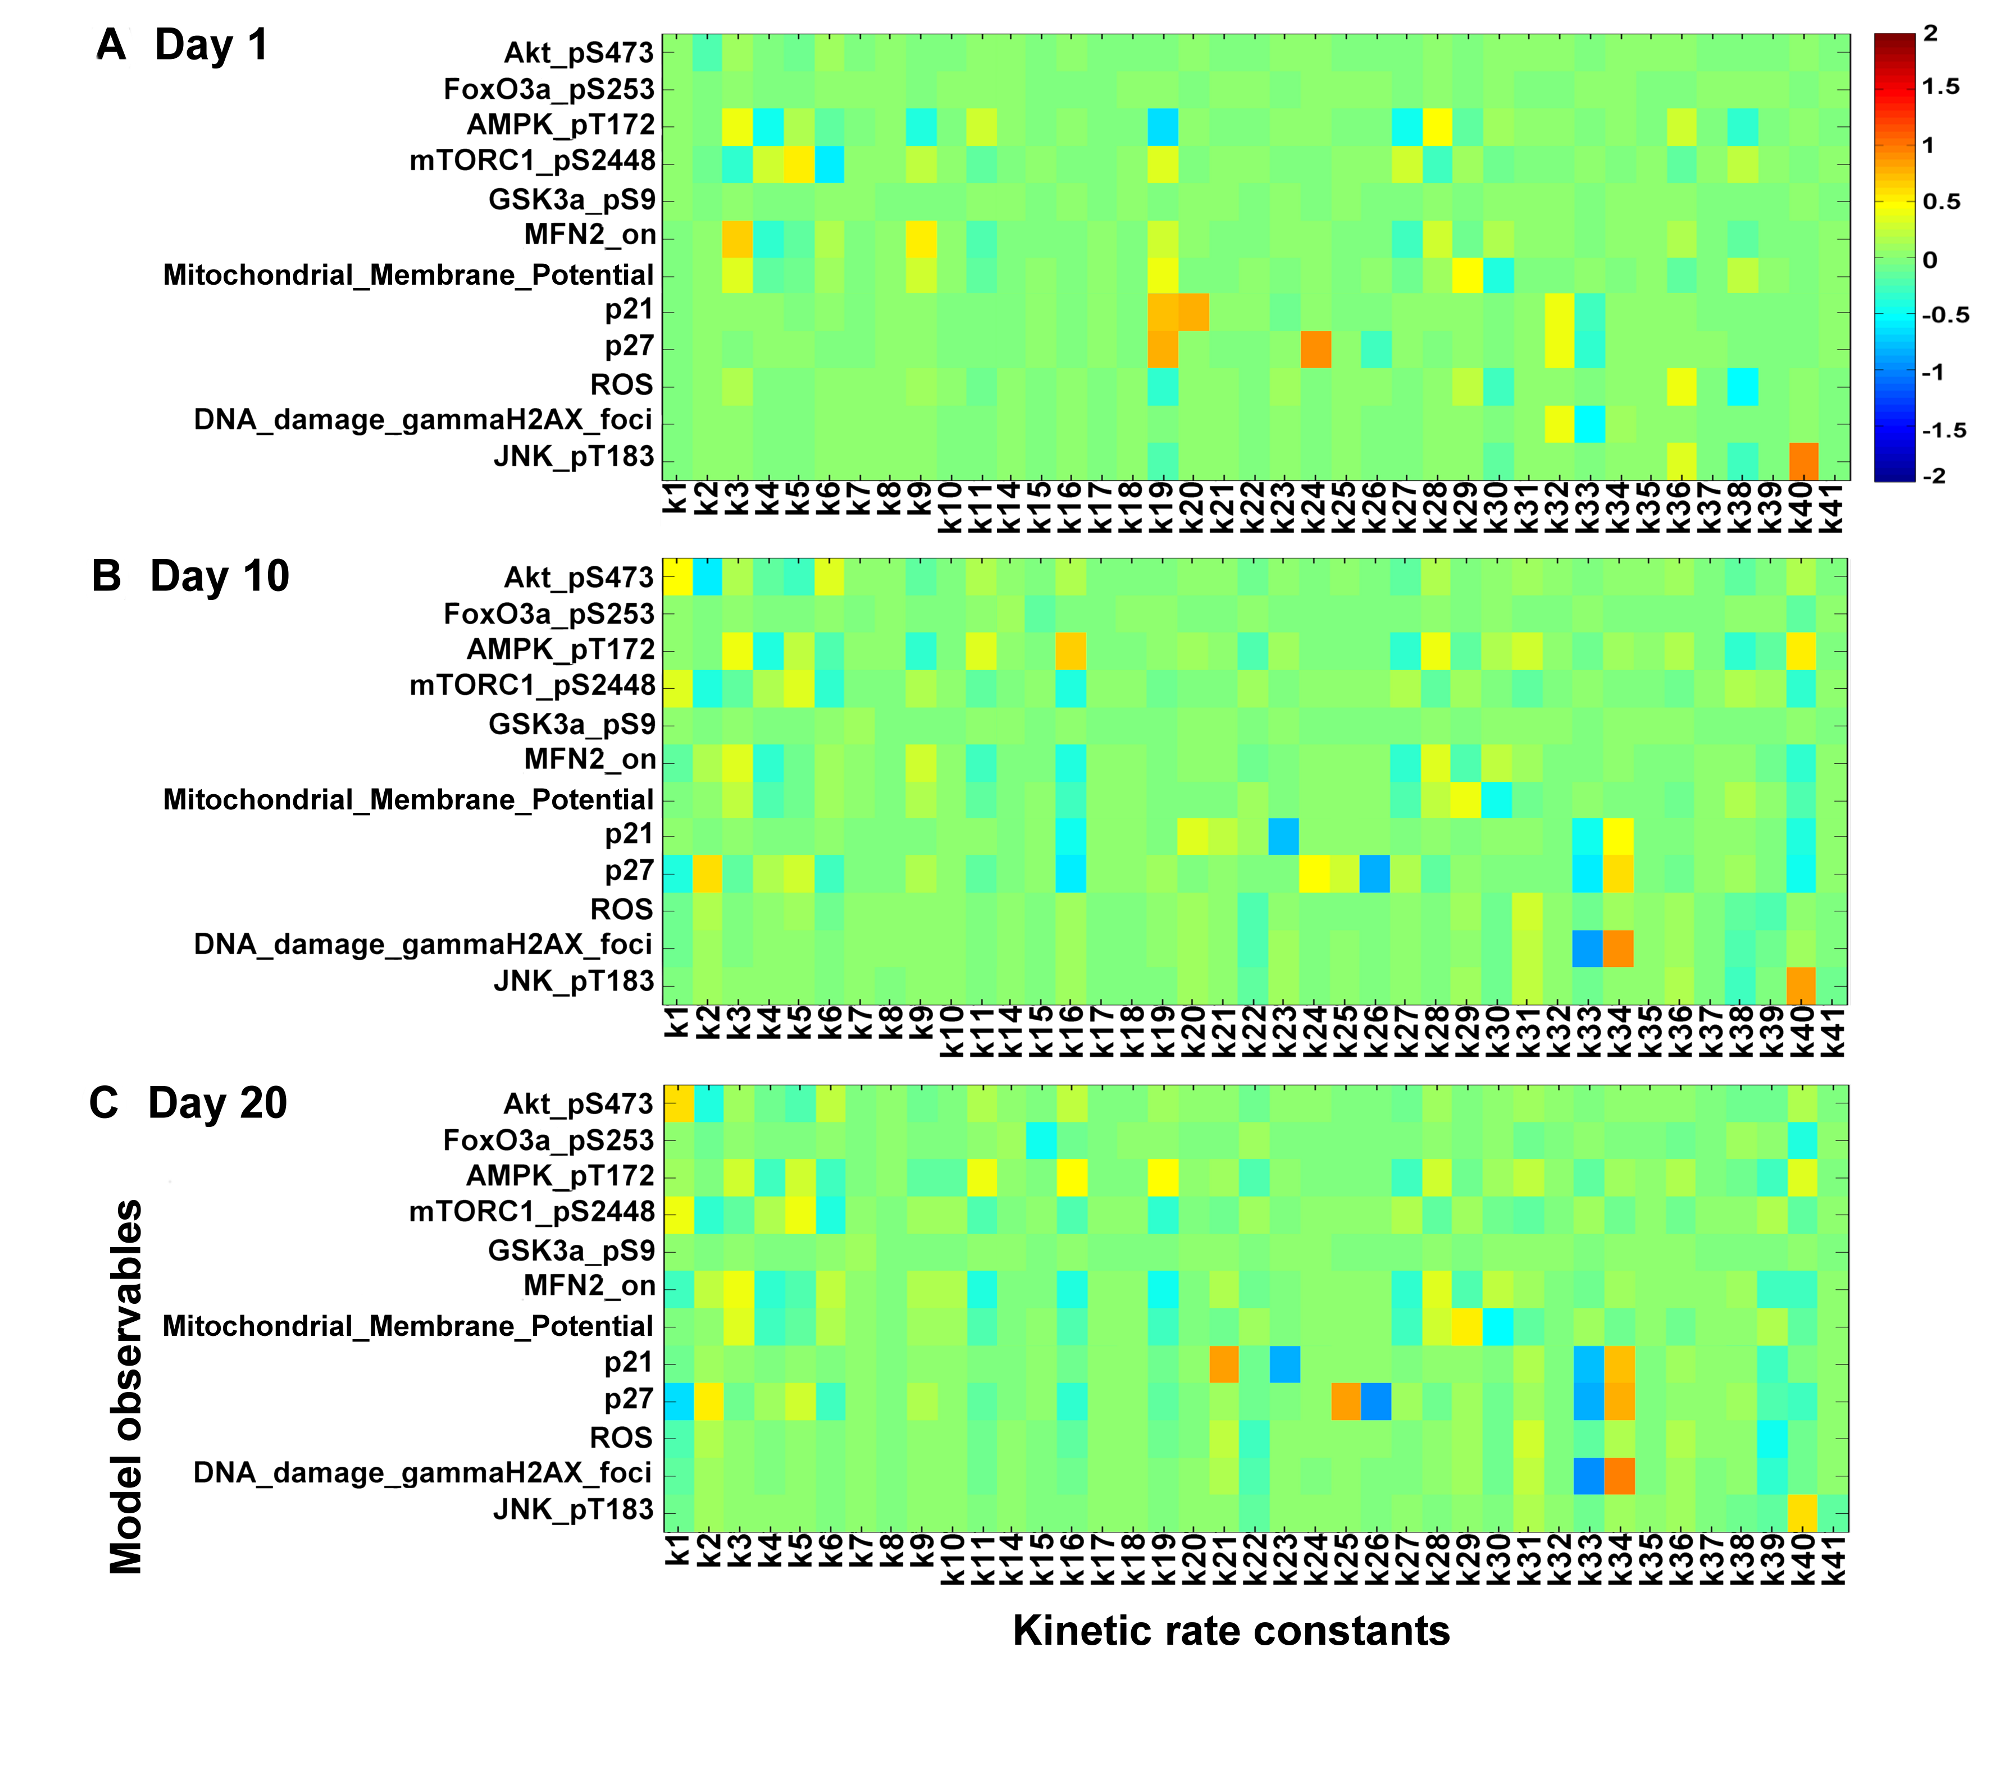
\includegraphics[scale=0.8]{sensitivity_analysis.png}
		\caption[Model sensitivity analysis]{Model sensitivity analysis. Sensitivity analysis was calculated in order to measure the contribution of the kinetic rate constant parameters over the model observable variables. The analysis was performed at day 1 (representing normal cells population, panel A), day 10 (mixed cells population, panel B) and day 20 (senescent cells population, panel C) post irradiation. From day 1 to day 20, Mfn2 showed a decrease in sensitivity by AMPK (k3) and by nuclear FoxO3a when unphosphorylated by JNK (k9). Interestingly, the system presented an increase in the sensitivity of the parameters controlling DNA damage: DNA repair (k33) and DNA damage generated by ROS (k34).}
		\label{fig:project3_sensitivity_analysis}
	\end{center}
\end{figure}
\clearpage




%\section{Tables}
%\label{project3-sec:Tables}

\begin{table}[tb]
	\begin{center}
		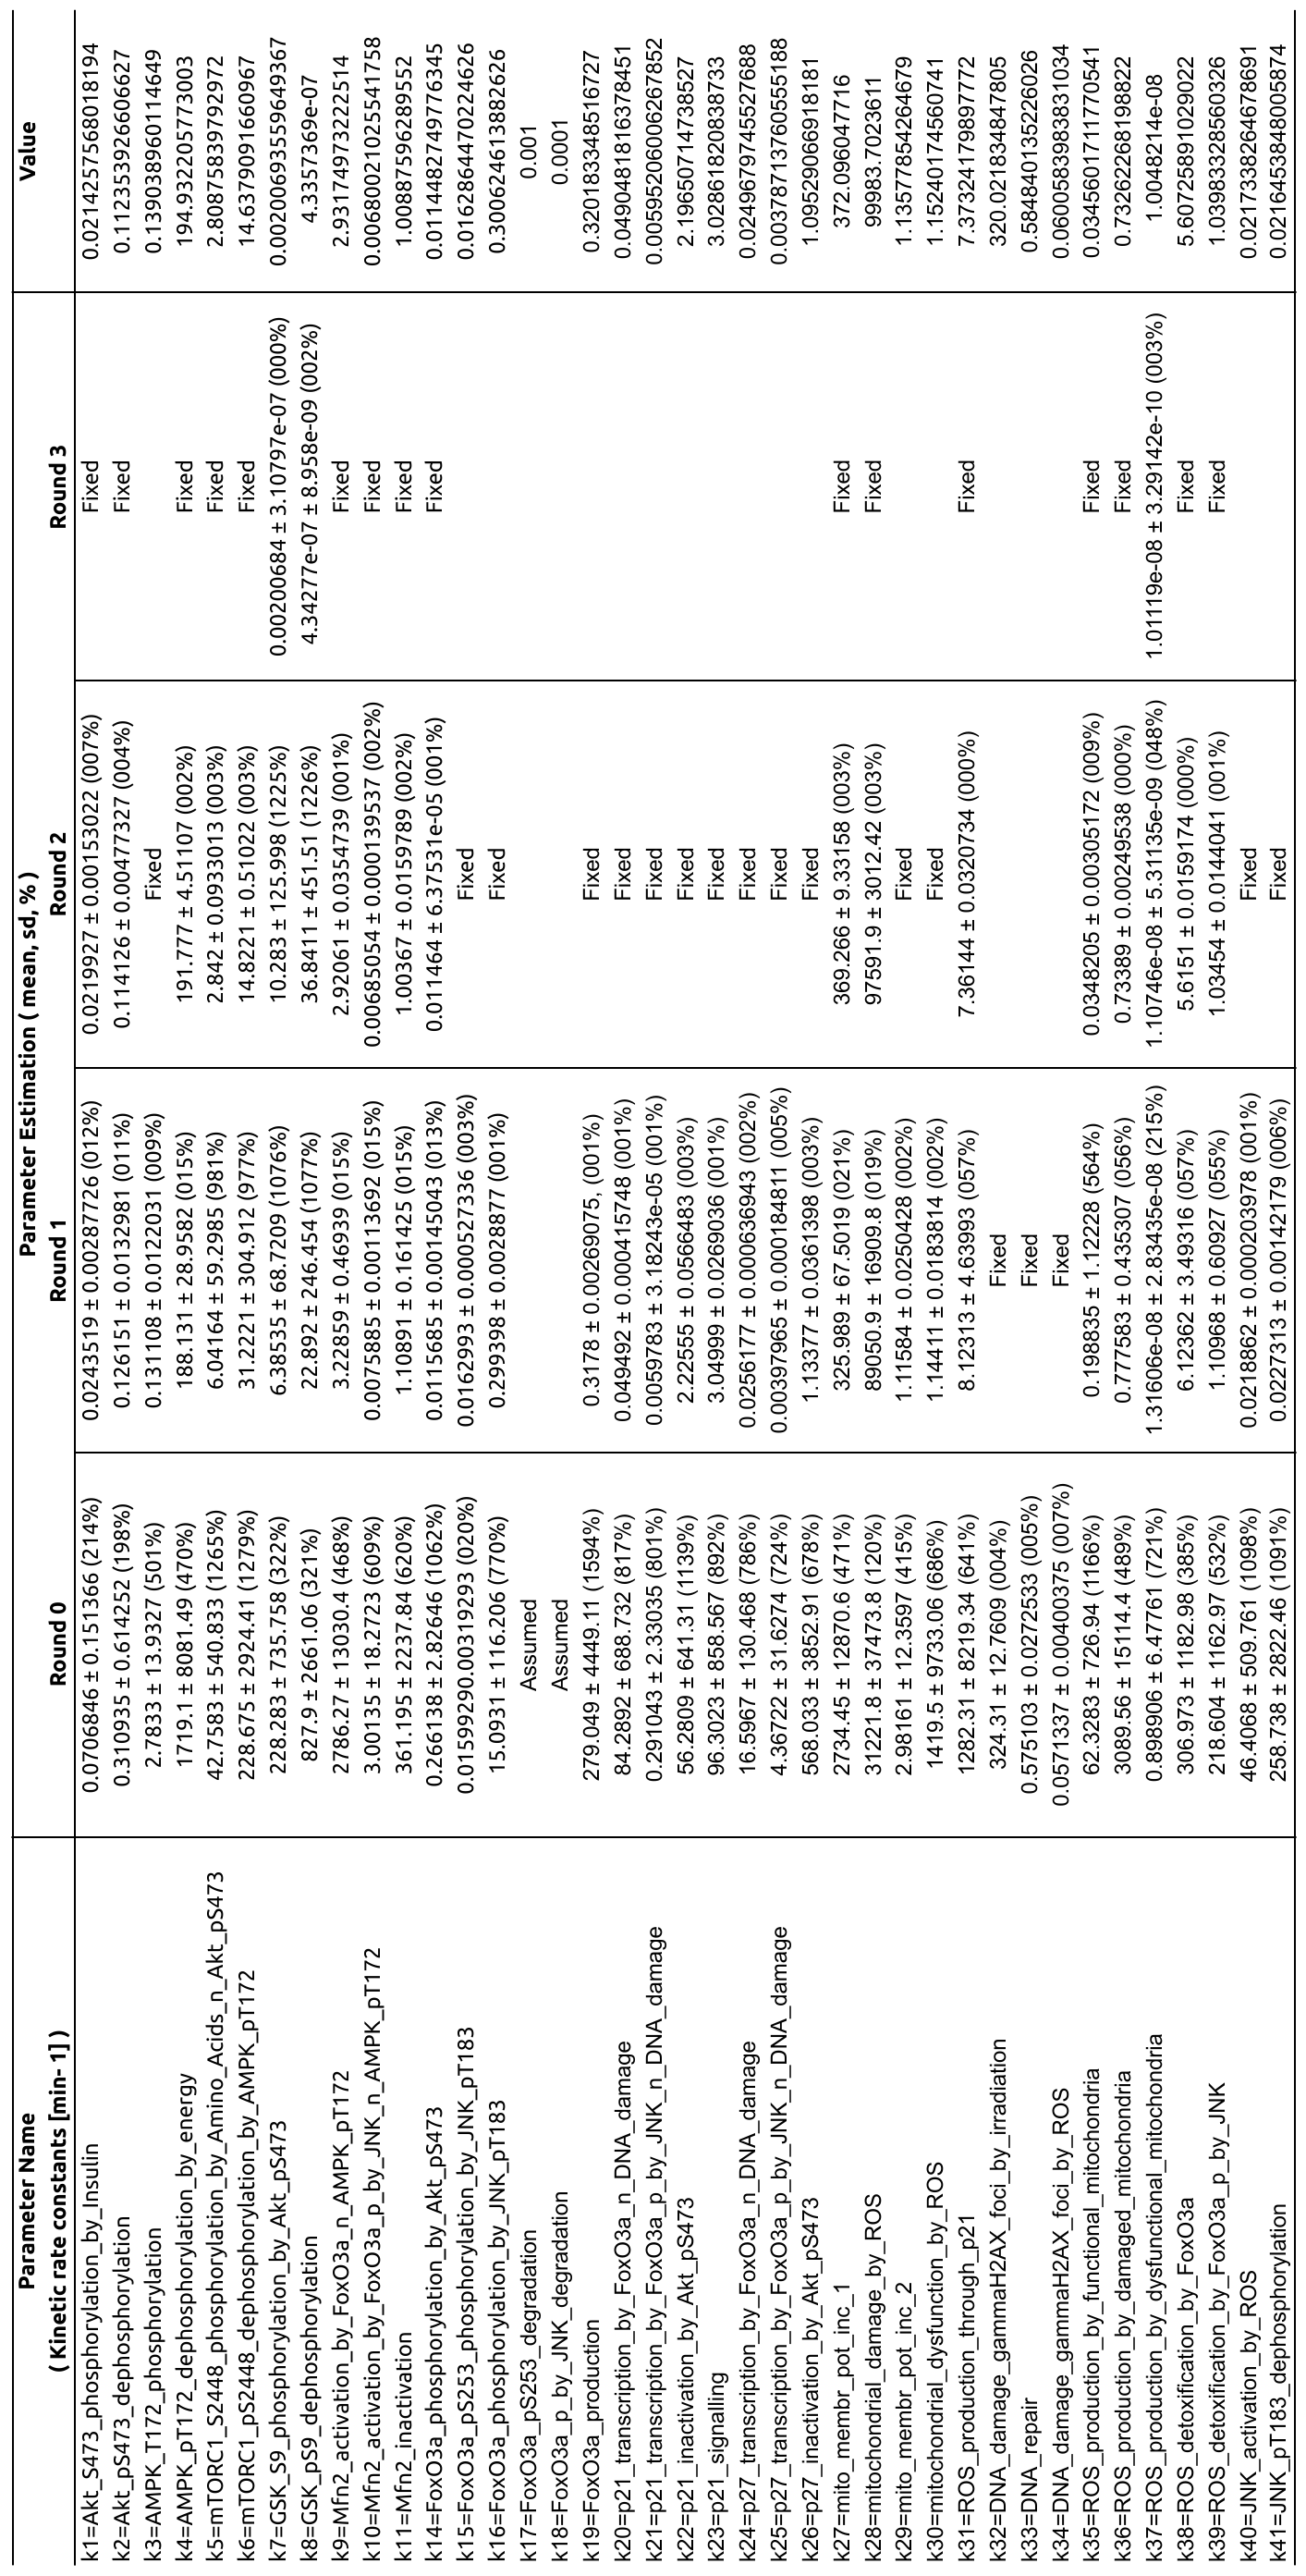
\includegraphics[width=3.8in]{kinetic_rate_constants_table.png}
		\caption[Table of the kinetic rate constants]{Table of the kinetic rate constants. Kinetic rate constants values and confidence intervals were estimated in 4 calibration rounds. For each round a sequence of 1000 fits was generated by perturbing the parameters initial values with noise of $10^{d*eps}$, where $d=1$ and $eps$ randomly chosen from a normal distribution $N(0,1)$. The best 350 fits of the sequence were selected and MOTA non-identifiability analysis was employed for determining tuples of related parameters requiring further calibration. At each round, the identified parameters were fixed and their mean, standard deviation and confidence interval were reported.}
		\label{tab:project3_kinetic_rate_constants_table}
	\end{center}
\end{table}
\clearpage

\begin{table}[tb]
	\begin{center}
		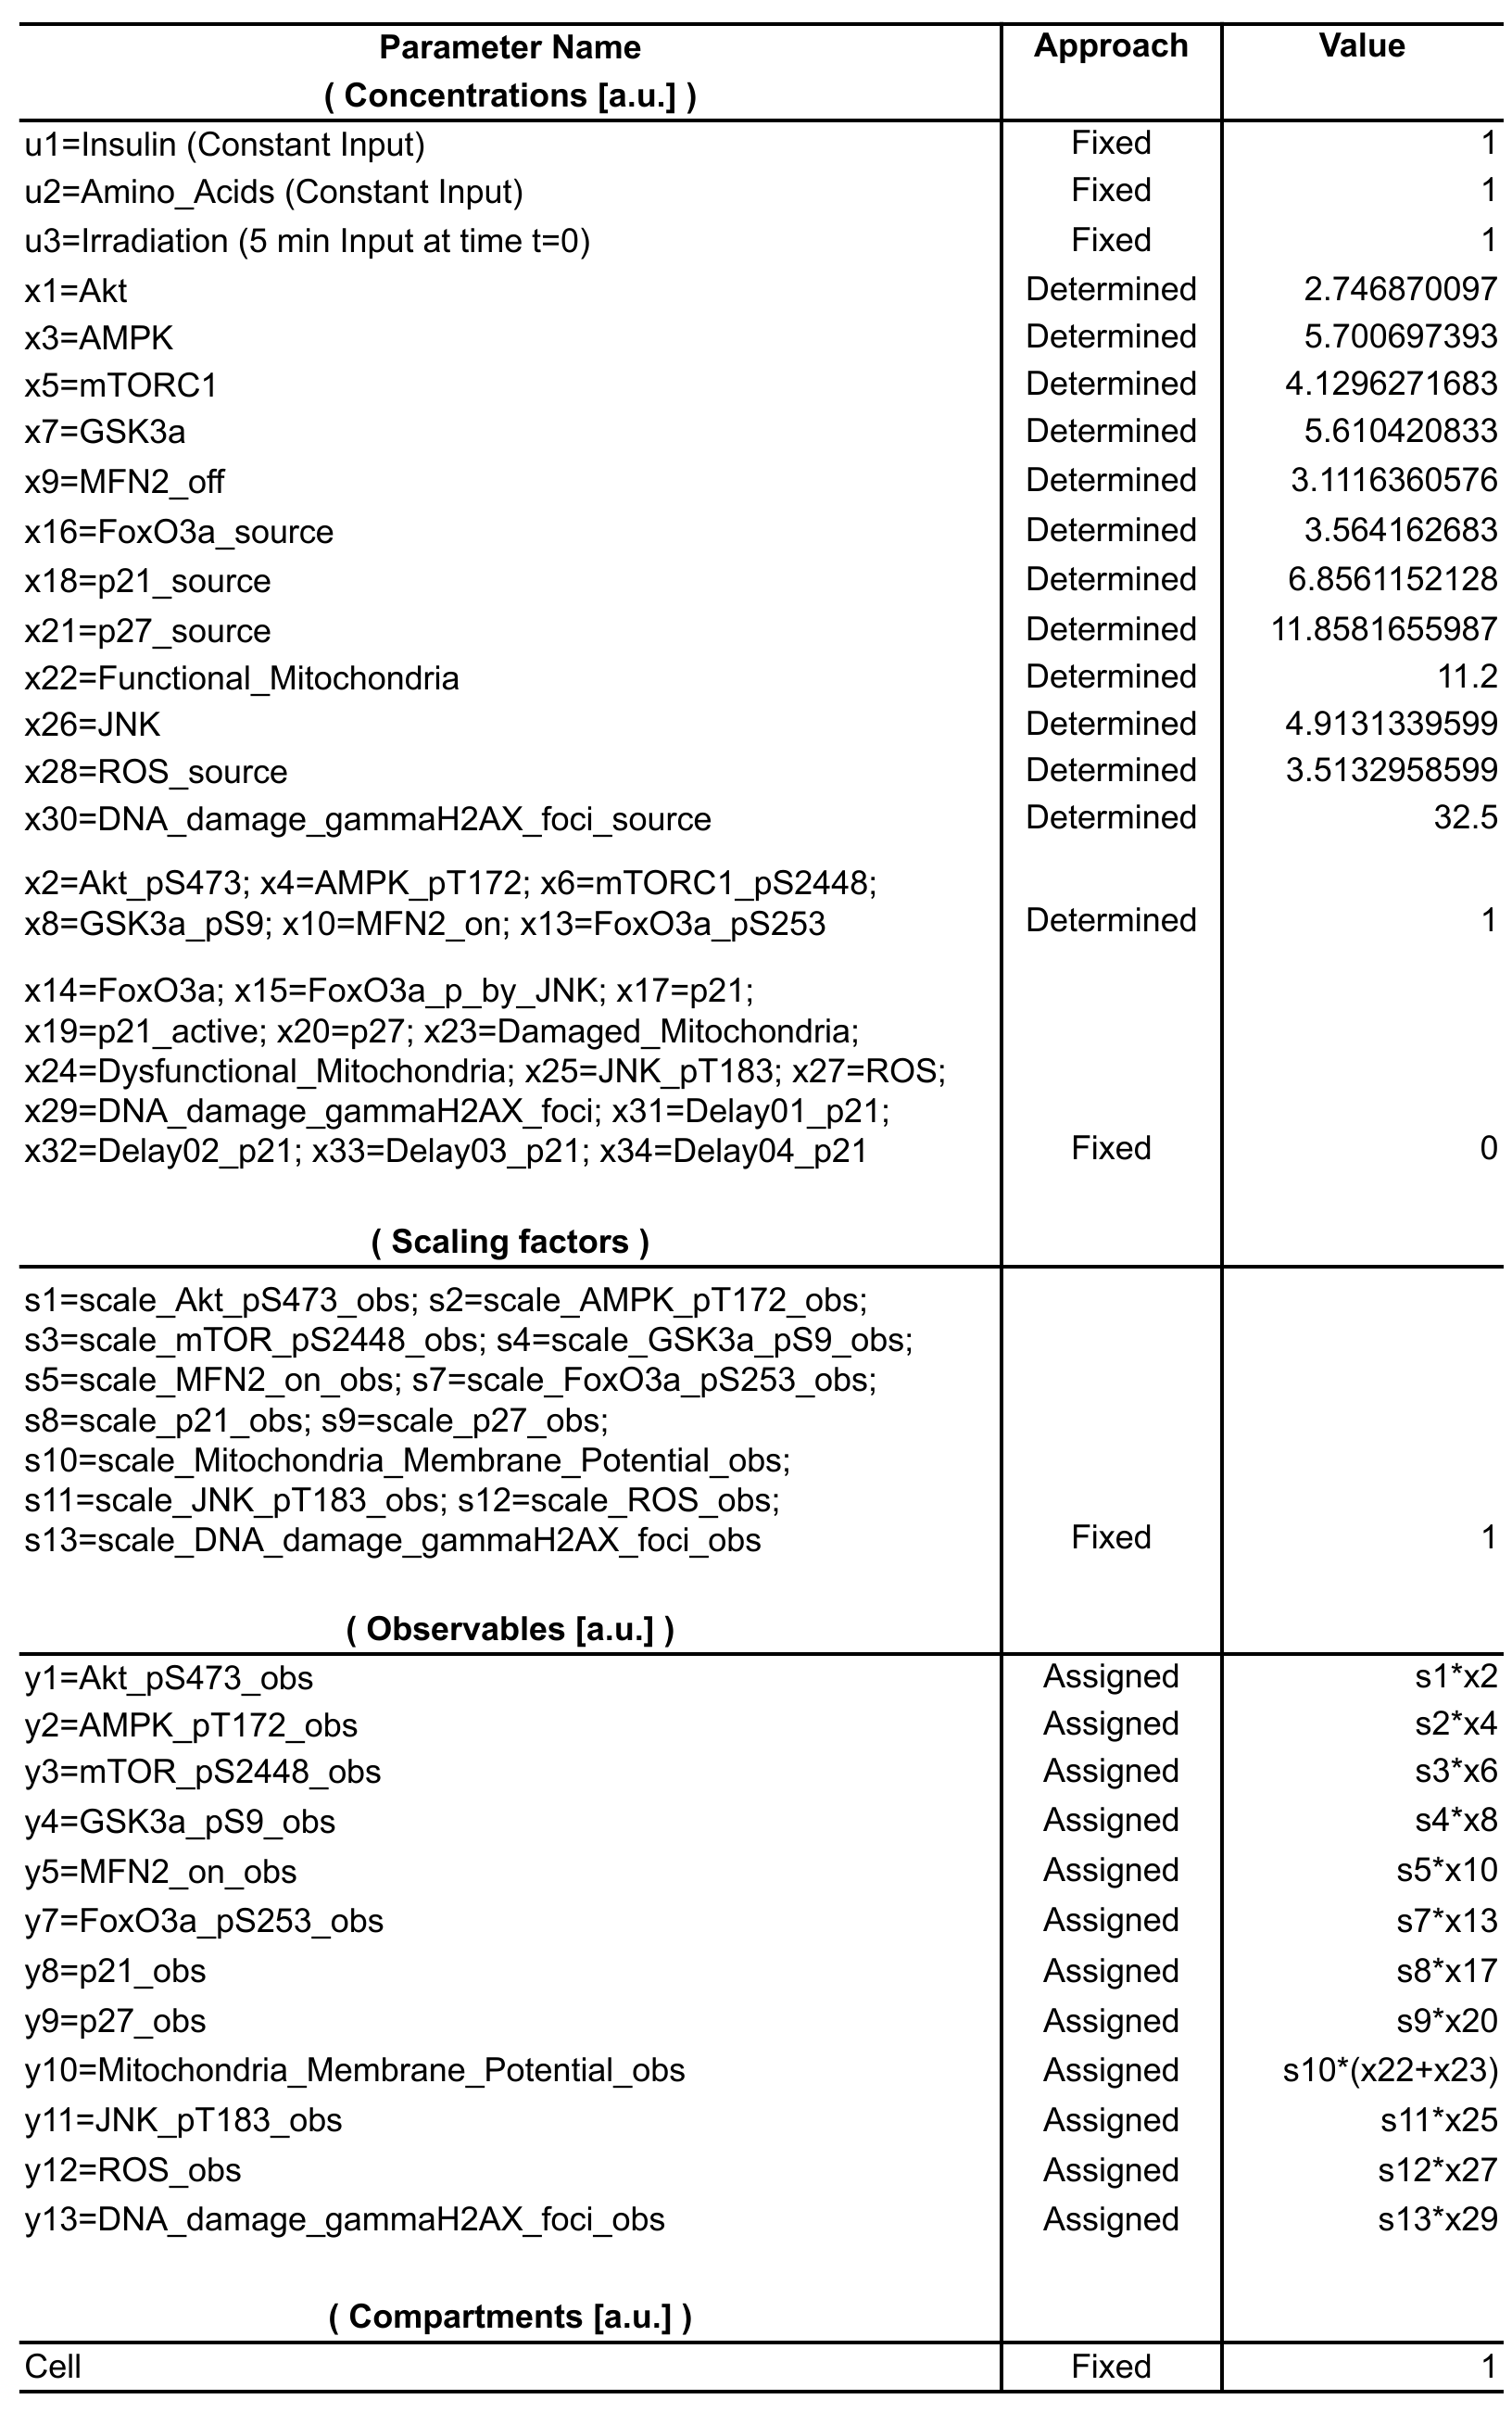
\includegraphics[width=3.4in]{concentrations_table.png}
		\caption[Table of the initial concentrations and auxiliary parameters]{Table of the initial concentrations and auxiliary parameters. Protein initial concentrations were directly determined from experimental time course data. Initial concentrations of protein inactive states were calculated as the maximum peak of the relative activation level in the time course plus two times the standard deviation at that time point. Since at time t=0 cells were treated with X-rays irradiation, the initial concentrations of active states for proteins in the oxidative stress signalling were fixed to 0. The remaining initial concentrations were fixed to 1 in accordance with the normalised experimental basal level, since cells were not starved of amino acids and insulin. In Figure \ref{fig:project3_senescence_model}, the three states of mitochondrial membrane potential (high, low, null) are here mapped with the species identifiers x22, x23 and x24, respectively.}
		\label{tab:project3_concentrations_table}
	\end{center}
\end{table}
\clearpage

\begin{table}[tb]
	\begin{center}
		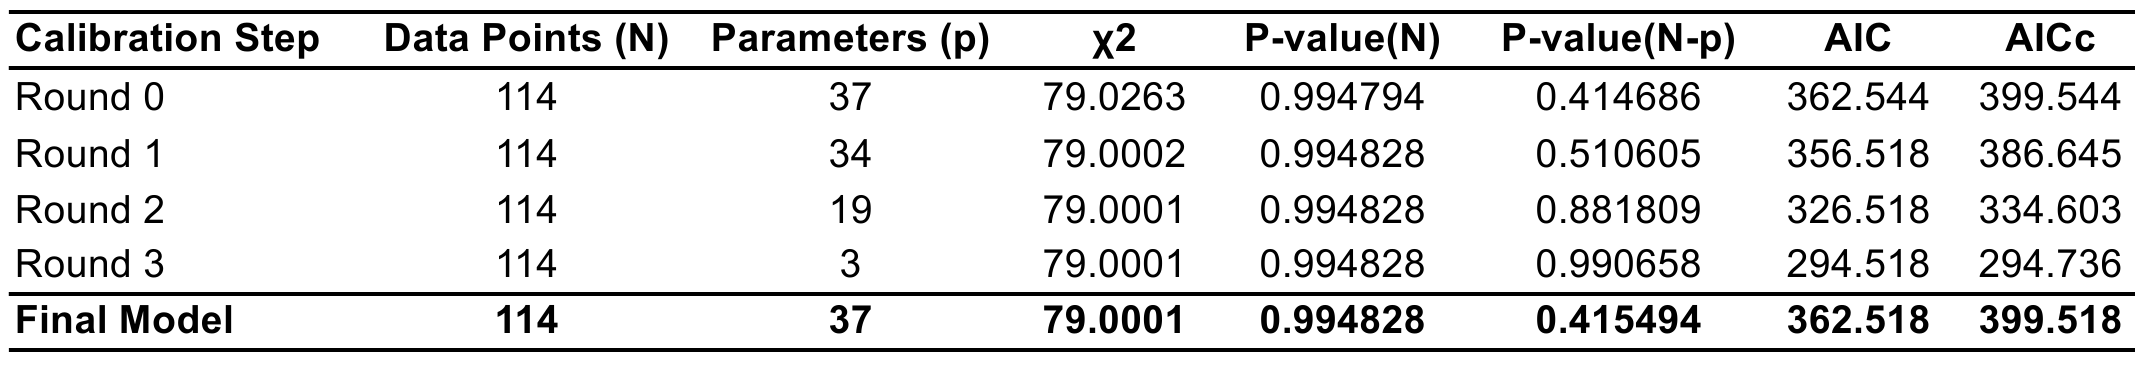
\includegraphics[width=5.4in]{rounds_chisquare_table.png}
		\caption[Model fit details for each calibration round]{Model fit details for each calibration round. For each calibration round, the measures of $\chi^2$, Akaike information criterion (AIC, AIC corrected) and Bayesian information criterion (BIC) are indicated. Since Round 0, the model was not statistically rejected (P-value(N-p) $>$ 0.05) and showed an accurate fitting with the data. Despite being required for parameter identification, the calibration rounds did not introduce significant improvements in the overall model fitting (see $\chi^2$, P-value(N) between Round 0 and Final Model). Between rounds the measures P-value(N-p), AIC, AICc and BIC showed improvements due to the decrease in parameters number p.  P-value(N), p-value(N-p): $\chi^2$ tests with $N$ or $N-p$ degrees of freedom, where $N$ is the number of fitted data points and p corresponds to the number of fitted parameters.}
		\label{tab:project3_rounds_chisquare_table}
	\end{center}
\end{table}
\clearpage

\begin{table}[tb]
	\begin{center}
		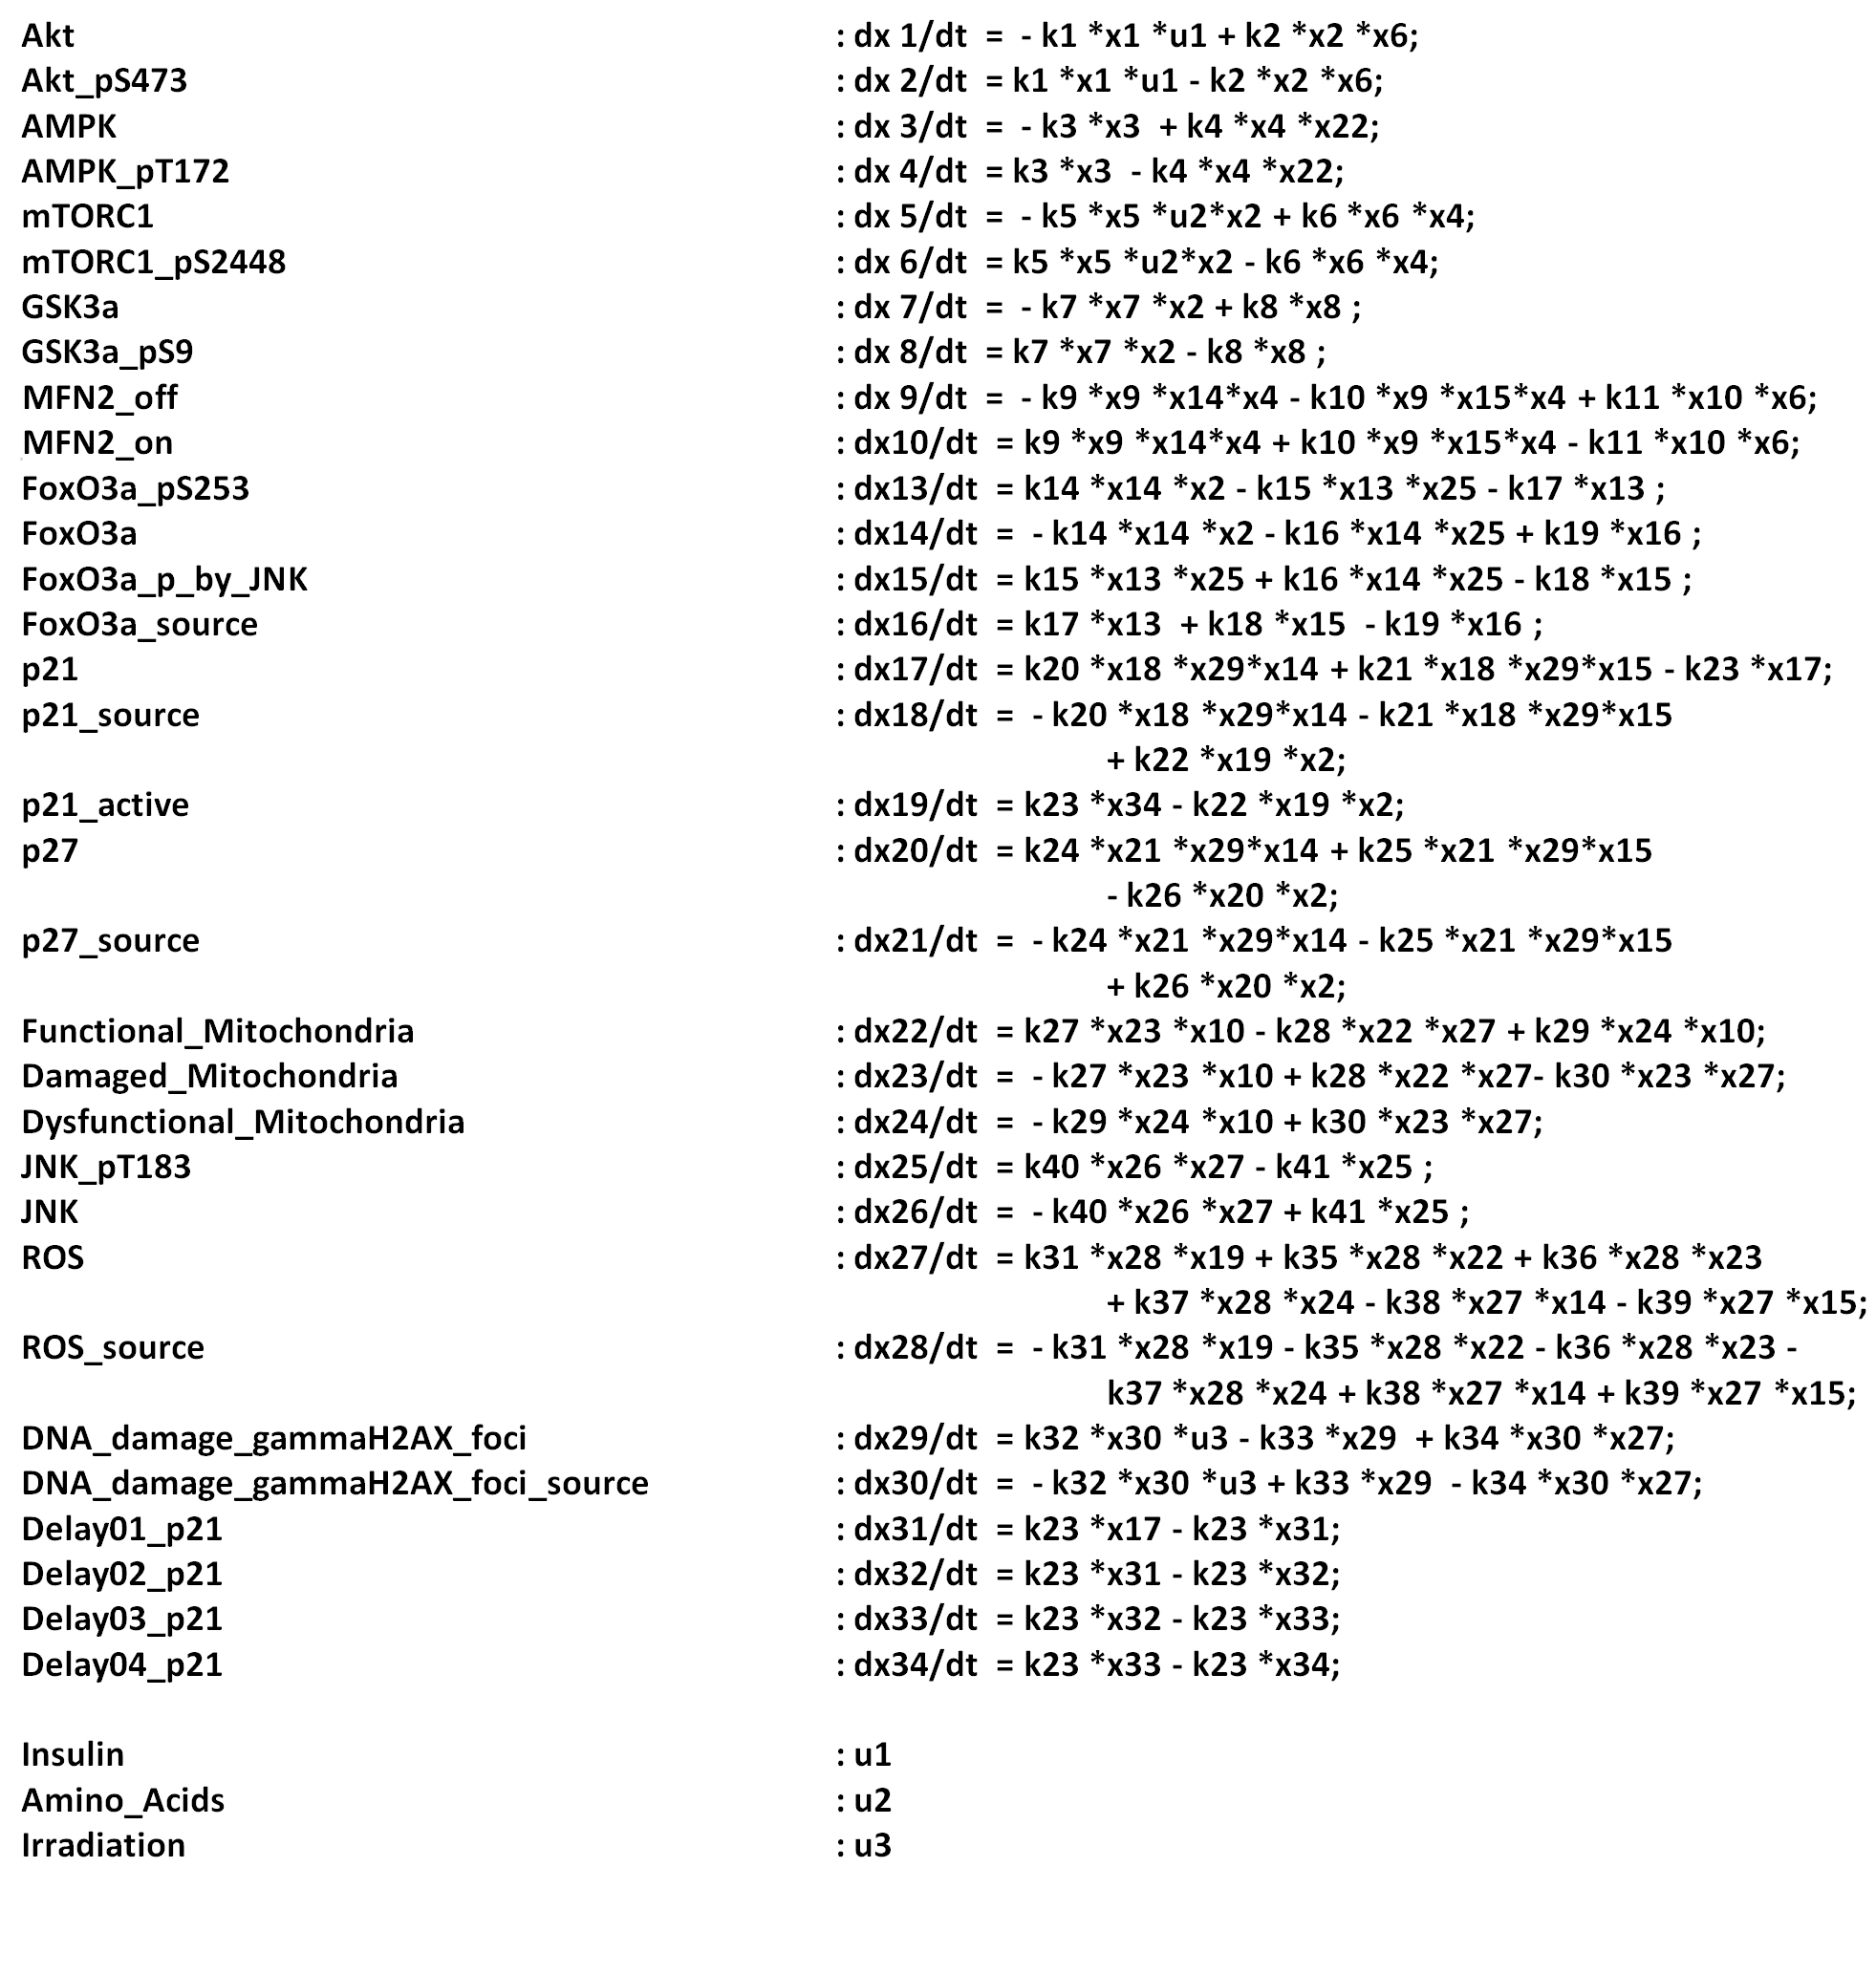
\includegraphics[width=5.5in]{ode_table.png}
		\caption[Ordinary differential equations of the model]{Ordinary differential equations of the model. List of the ordinary differential equations (ODEs) for the model. Kinetic rate constants were abbreviated using the notation shown in Table \ref{tab:project3_kinetic_rate_constants_table}. Protein activation states (species) are reported from Table \ref{tab:project3_concentrations_table}.}
		\label{tab:project3_ode_table}
	\end{center}
\end{table}
\clearpage

\begin{table}[tb]
	\begin{center}
		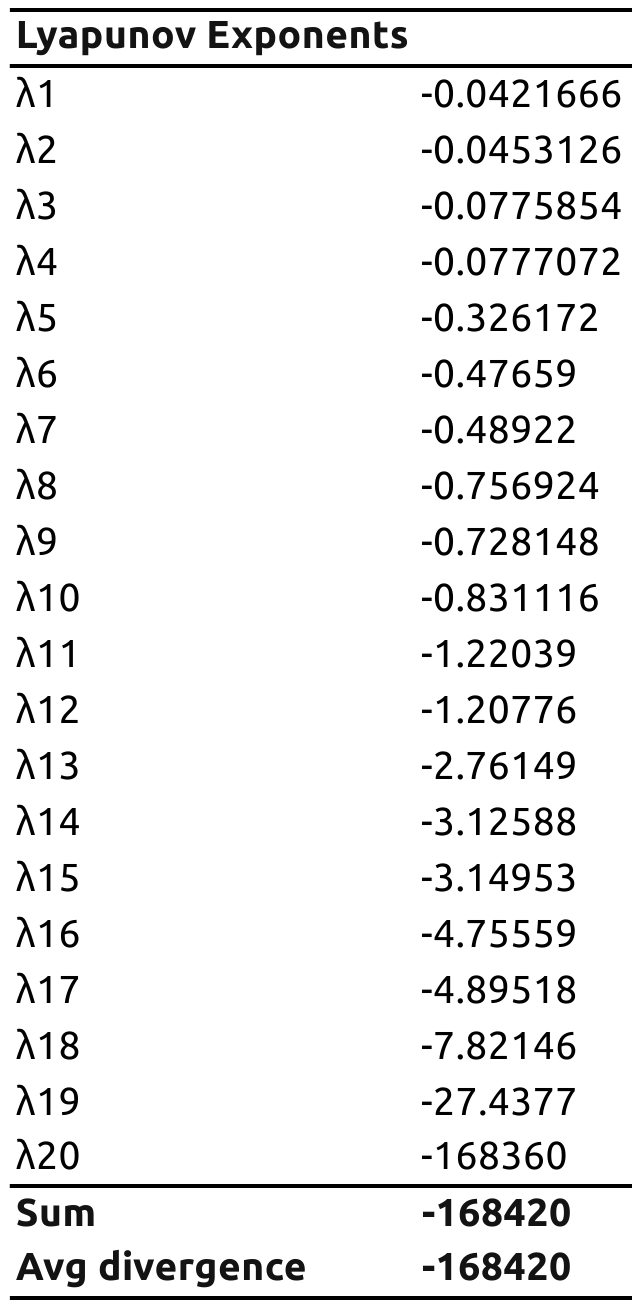
\includegraphics[width=1.8in]{lyapunov_exp.png}
		\caption[Lyapunov exponents of the model]{Lyapunov exponents of the model. The modelled system of first approximation is regular since all the coefficients are constant. The Lyapunov exponents computed for this model are all negative, indicating that the model is asymptotically Lyapunov stable and therefore the trajectories eventually converge to an equilibrium. The maximum Lyapunov exponent ($\lambda20$) is significantly high because the value for the variable \emph{Functional Mitochondria} ($x22$) dramatically dropped due to the initial irradiation and did not restore due to the high levels of ROS and DNA damage. The 20 Lyapunov exponents were computed for the reduced system (20 independent variables) using Copasi \citep{Hoops2006} and the inner Wolf method \citep{Wolf1985} was configured with parameters: orthonormalisation interval: 0.0001, overall time: 50, relative tolerance: 1e-06, absolute tolerance: 1e-10, maximum internal steps: 10000. The divergence computed using finite divergences 
(algorithm defined in \citep{Hindmarsh1983} and implemented in Copasi) coincides with the sum of Lypunov exponents indicating high confidence in the computation of the exponents.}
		\label{tab:project3_lyapunov_exp}
	\end{center}
\end{table}
\clearpage



% ------------------------------------------------------------------------


%%% Local Variables: 
%%% mode: latex
%%% TeX-master: "../thesis"
%%% End: 
